\documentclass[11pt,a4paper,spanish]{book}
\usepackage[a4paper,left=3cm,right=2cm,top=3cm,bottom=2cm]{geometry}
\usepackage{graphicx}
\usepackage[T1]{fontenc}
\usepackage[utf8]{inputenc}
\usepackage[spanish]{babel}
\usepackage{natbib}
\usepackage{multirow}
\usepackage[hyphens]{url}
\usepackage{hyperref}
\usepackage{appendix}
\usepackage{listings}
\usepackage{booktabs}% http://ctan.org/pkg/booktabs
\usepackage{pdfpages}

%todo---------------------------------
\usepackage{caption}
\usepackage{float}
\usepackage{xargs}                  
\usepackage{color}
\usepackage[colorinlistoftodos,prependcaption]{todonotes}
\newcommandx{\cambiar}[2][1=]{\todo[inline,linecolor=red,backgroundcolor=red!25,bordercolor=red,#1]{#2}}
\newcommandx{\agregar}[2][1=]{\todo[inline,linecolor=blue,backgroundcolor=blue!25,bordercolor=blue,#1]{#2}}

\definecolor{lightgray}{rgb}{.9,.9,.9}
\definecolor{darkgray}{rgb}{.4,.4,.4}
\definecolor{purple}{rgb}{0.65, 0.12, 0.82}

\newcommand{\tabitem}{~~\llap{\textbullet}~~}


\renewcommand{\appendixpagename}{Anexos}
\renewcommand{\appendixtocname}{Anexos}
\renewcommand{\appendixname}{Anexo}

\begin{document}

%\listoftodos[Todo-list]

\renewcommand{\tablename}{Tabla}
\renewcommand{\listtablename}{Índice de tablas}


%Empieza la numeración en números romanos
\frontmatter
% Incluimos la carátula
%Observación: Si bien la página del prefacio dice que sea empty, debería comenzar alli la numeración. Se sugiere numeración romana. Recomenzar la numeración en el primer capítulo de la tesis  con numeración arábiga.

\titlepage

\begin{center}
\ \\
\ \\
\vspace{-1cm}
 

\ \\

\vspace{0.5cm}
{\Large{\bf \sc Universidad Nacional del Comahue}}\\

\ \\
{\Large { \sc Facultad de Informática}}\\

\vspace{-2.5cm}
\mbox{\hspace{-1cm}
\includegraphics[width=2.5cm,height=2.5cm]{img/unc.png}\hspace{13cm} 
\includegraphics[width=2.5cm,height=2.5cm]{img/fai.png}}


\vspace{6cm}

{\Large {\bf\sc Tesis de Licenciado en Ciencias de la Computaci\'on}}\\
\ \\
\ \\
{\LARGE {\bf Centro de cómputos de carga descentralizada como alternativa al sistema de elecciones}}\\
\vspace{3cm}


{\Large Silvia Vanesa Soto}\\
\vspace{2cm}

{\Large Claudio Vaucheret}\\
\ \\
{\Large Pablo Kogan}\\

\vfill
{\Large {\sc Neuqu\'en}\hspace{6cm}{\sc Argentina}}\\
\ \\

{\Large 2019}\\

\end{center}

\pagebreak





% Incluimos la página de prefacio.
\ \\
\ \\
\label{pagpref}
\noindent{\LARGE \sc Prefacio}\\
\ \\
\ \\

\ \\

\ \\
\ \\


Esta tesis es presentada como parte de los requisitos finales para optar al grado acad\'emico de {\em Licenciada en Ciencias de la Computación}, otorgado por la Universidad Nacional del Comahue, y no ha sido presentada previamente para la obtención de otro título en esta Universidad u otras. La misma es el resultado de la investigación llevada a cabo en el Departamento de Teoría de la Computación, de la Facultad de Informática, en el período comprendido entre Mayo 2019 y Junio 2022, bajo la dirección de Mg. Claudio Vaucheret y la codirección de Lic. Pablo Kogan.
\vspace{3cm}


\ \\
{\flushright Silvia Vanesa Soto\\
{\sc Facultad de Informática \\
Universidad Nacional del Comahue}\\
{\em Neuqu\'en, 8 de Julio de 2022.}\\}

\vfill

\begin{center}
%
\framebox{\begin{minipage}[t]{0.9\columnwidth}%
\begin{flushleft}

\includegraphics[scale=0.035]{img/unc.png}

\vspace{-2cm}
{\large \hspace{5cm}\sc universidad
nacional del comahue} \\
\par\end{flushleft}
\begin{center}
{\large \qquad{}}{ \hspace{2.5cm} Facultad de Informática}
\par\end{center}

\vspace{1cm}

\indent \ \ \ \ \ \ \ \ \ \ \ La presente tesis ha sido aprobada el día ........................., mereciendo la \\
\indent \ \ \ \  \ \ \ \ \ calificación de .............................

\medskip{}

\vspace{1cm}
\end{minipage}}
\end{center}

\pagebreak


% Incluimos la página de dedicatorias. Esta página es opcional.
% Si la página no quiere ser incluida anteponga el símbolo "%" al comienzo de la siguiente línea
%\ \\
\ \\
\label{pagdedic}
\noindent{\LARGE \sc Dedicatorias}\\
\ \\
\ \\

\ \\

\ \\
\ \\
Aqu\'i van las dedicatorias del alumno. Esta página es opcional.\\

\vfill
\pagebreak



% Incluimos la página de agradecimientos. Esta página es opcional.
% Si la página no quiere ser incluida anteponga el símbolo "%" al comienzo de la siguiente línea
%\ \\
\ \\
\label{pagagrad}
\noindent{\LARGE \sc Agradecimientos}\\
\ \\
\ \\

\ \\

\ \\
\ \\
Aqu\'i van los Agradecimientos del alumno. Esta página es opcional.\\

\vfill
\pagebreak


% Incluimos la página de resumen
\ \\
\ \\
\label{pagresum}
\noindent{\LARGE \sc Resumen}\\
\ \\
\ \\

\ \\

\ \\
\ \\

 \cambiar{...pk o cv casos para cambiar...}
 \agregar{...pk o cv casos que agregar...}
 En estos tiempos, donde la tecnología forma parte de nuestra rutina y en muchos casos se confía plenamente en ella, podemos decir que nos ayuda a automatizar múltiples procesos y reduce los tiempos de nuestras tareas. En los últimos años se ha introducido tecnología en procesos electorales del ámbito universitario, municipal, provincial, nacional e internacional. Los sistemas electorales se pueden definir como sistemas críticos donde una falla puede ser irreversible y con un gran costo. Las leyes Argentinas imponen que el voto sea universal, igualitario, secreto y obligatorio. Un sistema de votación exitoso debe lograr la confianza de toda persona involucrada en el proceso: ciudadanos, partidos políticos y gobierno. Por este motivo, la voluntad del elector es el dato más importante en este sistema, una falla en su conteo o no procesar correctamente el voto emitido puede generar errores que se propagan en el escrutinio de todo el comicio y puede darnos un resultado equivocado.\newline
 El proceso electoral comienza cuando se definen las fechas de oficialización de padrones y listas, pasando luego por el acto electoral, escrutinio y proclamación de autoridades elegidas. Por lo tanto, una falla en cualquiera de estas etapas provocaría que se pierda la confianza en de todo el proceso.\newline
 En esta tesis se evalúan las propiedades que deben protegerse dentro de un sistema electoral y cómo impacta la tecnología a cada una de ellas, analizando experiencias de elecciones a nivel municipal e internacional. A partir de esta evaluación se presenta un sistema que mantiene la emisión del voto en papel de cada elector, y el escrutinio manual por parte de las autoridades de mesa. Con el objetivo de mejorar los tiempos del proceso de cómputo, sin poner en riesgo la confianza del sistema y garantizar el secreto del voto, se desarrolla la propuesta de ``acta electrónica'' denominada Gukena, donde cada autoridad de mesa luego de su escrutinio manual realiza la carga de esta información.\newline
 Gukena ha sido utilizado en el ámbito de la Universidad Nacional del Comahue a partir del 2015. Este sistema resolvió el cómputo de los votos que, previo a esta fecha, se realizaba manualmente por una única persona encargada de ingresar los datos, gestionar correctamente los resultados y distribuir los cargos. La forma de trabajo generaba un cuello de botella en la carga de los datos y una demora de varias horas y hasta días en obtener los resultados finales.\newline
 Esta herramienta permitió agilizar el escrutinio final debido a la carga descentralizada y sin afectar la claridad de la información enviada. Se logró reflejar los resultados provisorios de todas las mesas en el instante en que cada autoridad de mesa enviaba los datos. \newline
 Por último en este trabajo se realiza una comparación de velocidad de carga entre las elecciones provinciales de Río Negro, Neuquén y Córdoba contra el sistema Gukena. 

\vfill
\pagebreak


% Incluimos la página de resumen en inglés
\ \\
\ \\
\label{pagsumm}
\noindent{\LARGE \sc Abstract}\\
\ \\
\ \\

\ \\

\ \\
\ \\

Currently, technology is part of our routine and in many cases it's fully trusted, we can say that it helps us to automate multiple processes and reduces the time to do our tasks. In recent years, technology has been introduced into university, municipal, provincial, national and international elections. Electoral systems are crytical systems where a failure can be irreversible and costly. Argentine law requires that the vote be universal, equal, secret and compulsory. A successful voting system must have the trust of everyone involved in the process: citizens, political parties and government. For this reason, the voter's will is the most important element in this system, a mistake in counting it or a wrong processing of it can generate errors that can propagate in the scrutiny of the whole election and give us a wrong result.\newline
The electoral process initiates when the officialization of the lists of voters and the electoral rolls are defined, throughing the electoral act, scrutiny and the proclamation of the elected authorities. Therefore, a failure in any of these steps could make the entire process become trustless.\newline
This thesis evaluates the properties that must be protected inside an electoral system and how technology impacts each of these properties, analyzing experiences of elections at a municipal and international level. After this evaluation, a system is presented that maintains the paper ballot emission of each voter, and the manual scrutiny by the authorities of the electoral table. In order to improve the time of the counting process, without the risk of the loose a system confidence and to guarantee the secrecy of the vote, the proposal of ``electronic certificate'' called Gukena has been developed, where each table authority, after the manual counting of votes, submitted this information.\newline
Gukena has been working at the National University of Comahue since 2015. This system resolved the counting of votes, which before this date, was doing manually by a single person in responsible for registering the information, managing the results correctly and distributing the roles. This way of working generated a bottleneck in filling the data and it had delay of several hours or even days to get the final results.\newline
This tool helped to reduce the time required for the final scrutiny due to the decentralized uploading and without affecting the transparency of the information submitted. Provisional results were reflected as soon as each voting table authority submitted the information.\newline
Finally, this document compares the loading velocity between the provincial elections of Río Negro, Neuquén and Córdoba in relation to the Gukena system.

\vfill
\pagebreak


% Tabla de contenido o Indice del contenido
\tableofcontents{}

% Lista de figuras o Indice de figuras
\listoffigures

% Lista de tablas o Indice de Tablas
\listoftables

%Empieza la numeración en números arábigos
\mainmatter
\label{Introduccion}
\chapter{Introducción}
El sistema electoral argentino debe asegurar que la votación sea universal, igual, secreto y obligatorio \citep{arlettaz2012libertad}. El proceso electoral comienza cuando se definen las fechas de oficialización de padrones y listas, acto electoral, escrutinio provisorio, escrutinio definitivo y proclamación de autoridades electas. Se considera que un sistema de votación exitoso debe cumplir el principal objetivo que es construir la confianza de toda persona involucrada en el proceso: ciudadanos, partidos políticos, gobierno, entre otros. Como posibles alternativas en este proceso, planteadas a nivel mundial, ha sido aplicar distintas técnicas para computarizar parte del proceso de votación. Existen diferentes dominios con antecedentes a estas técnicas, tanto en Argentina, como en  otros  países,  con  distintos  sistemas  de  voto  electrónico. Tomando estas experiencias y el objetivo principal que debe cumplir un sistema electoral, se parte de la idea de generar un sistema que mantenga la separación física del votante con la tecnología, y forzar un escrutinio manual por parte de las autoridades de mesa en el momento del conteo. \newline
En este capítulo se presenta la motivación, objetivos y organización de la tesis.

\section{Motivación}
Antes del 2015, el cómputo provisorio de los votos en la Universidad Nacional del Comahue (UnComa) se realizaba en forma manual por una persona, encargada de ingresar los datos en una planilla electrónica. Esta persona era responsable de gestionar correctamente los resultados y distribuir los cargos. La forma de trabajo generaba un cuello de botella en la carga de los datos y una demora de varias horas y hasta días en obtener los resultados finales. \newline
%\cambiar{ayudaría por ayudó, evitaría por evitó, permitiría por permitió. HECHO}
%\cambiar{Con el objetivo de mejorar los tiempos del proceso de cómputo, se desarrolla HECHO}
Con el objetivo de mejorar los tiempos del proceso de cómputo, se desarrolla la propuesta de ``acta electrónica'' basada en el proceso de carga electrónica del acta creada en papel, mediante un método descentralizado  por parte de cada autoridad de mesa. Dicha herramienta evitó el contacto del votante con un sistema electrónico, resguardando el anonimato del elector, y ayudó a que cada autoridad de mesa envíe los datos de manera rápida y transparente. De todos modos, el sistema no quita el envío de telegramas para validar la consistencia de los datos con su respectiva acta, por lo tanto existen validaciones que permite corregir cualquier desvío en los datos cargados en el sistema. Este herramienta permitió disminuir la demora del escrutinio final, sin afectar la claridad de la información enviada. Se logró reflejar los resultados provisorios de todas las mesas al instante que cada autoridad de mesa envió los datos.

\section{Objetivos de la Tesis}
El objetivo de la tesis es el diseño e implementación de un sistema de acta electrónica para el escrutinio descentralizado de elecciones. Con esto se pretende agilizar el recuento de votos y lograr un resultado provisorio disponible en tiempo real. Se analizará el impacto del uso de la tecnología en relación con el sistema electoral tradicional, evaluando experiencias en distintos ámbitos tanto con éxito como fracaso, permitiendo analizar y evaluar características que ayudaron o fracasaron dentro de un sistema real.\newline
Dicha herramienta permitirá cargar los datos obtenidos en cada punto de votación y luego validar su consistencia mediante la interacción con autoridades electorales. 

\section{Organización de la Tesis}
A continuación se describe la estructura de esta tesis:
\begin{enumerate}
    \item Capítulo \ref{SistemaElectoral}: revisión conceptual sobre las características y modelo sobre un sistema electoral tradicional.
    \item Capítulo \ref{Elecciones}: revisión sistemática de la utilización de tecnología en  Elecciones en diferentes dominios.
    \item Capítulo \ref{Gukena}: se describe el sistema desarrollado Gukena como opción en la utilización de las elecciones de la Universidad Nacional del Comahue.
    \item Capítulo \ref{Gukena2}: se exponen los resultados obtenidos luego de utilizarse Gukena en las diferentes elecciones realizadas en la Universidad Nacional del Comahue entre el 2015 y 2019.
\end{enumerate}

\section{Metodología}
La metodología que se utilizó para lograr los objetivos inició con un relevamiento de distintas fuentes bibliográficas estudiando y analizando características de un sistema electoral tradicional.
%\cambiar{Además se analizaron diferentes intentos ..... HECHO}
Además se analizaron diferentes intentos de incluir tecnología en el proceso de votación (votación electrónica) en ámbitos nacionales e internacionales. Con este conocimiento relevado y los contenidos de programación y aplicaciones enseñados y empleados en las primeras materias de programación, se analiza, diseña e implementa el software propuesto con el objetivo de satisfacer una gran parte de las propiedades deseables de un sistema electoral. Se realizaron distintos tests para verificar su funcionalidad finalizando con su inserción experimental en el sistema electoral real de la Universidad Nacional del Comahue. Esta herramienta se desarrolla con software libre y su código quedó disponible y abierta para futuras mejoras o investigaciones.

%\agregar{Metodologia: Podes tomar de referencia las tesis ejemplo que te mandé y la propuesta. -HECHO}
%1.3 Metodología de Nati
% La metodología que se utilizó para lograr los objetivos se apoyó en un estudio teórico/práctico de
% los contenidos de programación y aplicaciones, enseñados y empleados en las primeras materias de
% programación. También se estudiaron y se analizaron las distintas características de las herramientas
% basadas en software libre para elegir la más adecuada y realizar la reingeniería para el desarrollo,
% diseño e implementación del software propuesto. Se realizaron distintos tests para verificar el código
% y las salidas del programa. La prueba y validación de la herramienta se realizó en un laboratorio de
% desarrollador por un usuario final, alumnos y un profesor.
\chapter{Tecnología en el Proceso Electoral}
\label{SistemaElectoral}
\cambiar{No se describen todos los sistemas de votos existentes, y si se hace, están en forma muy resumida. No analiza ventajas y desventajas de cada uno (2.1.1). No se analizan los votos en papel sin uso de tecnología.}
\cambiar{Se habla de Boleta única de sufragio (BUS), Boleta única, Boleta única electrónica (BUE), boleta única en papel, etc. pero no se describe ninguna.}
\cambiar{Describe mecanismos de voto electrónico, pero no con sus características, sino con ejemplos de implementación. Deberían ser dos cosas diferentes.}
\cambiar{Faltan referencias que respalden los conceptos plasmados y las opiniones. En general se dan muchas opiniones, en su mayoría negativas, de los sistemas electorales nombrados sin fundamentos. Es decir, son opiniones del autor? se han analizado?}
\cambiar{A veces dice Figura, otras Gráfico, otras Imágen. Unificar Figura.}
\cambiar{En general: El capítulo advierte de una revisión conceptual de las características de un sistema electoral tradicional (según Capítulo 1). Sin embargo, luego se mezcla con la aplicación de tecnologías al sistema. No analiza y compara los sistemas de votos. Da opiniones sin fundamento.}

Involucrar tecnología en el proceso electoral es complejo, no sólo por sus desafíos técnicos, sino también por su importancia para el Estado y para la sociedad en general. Un sistema de voto electrónico involucra considerar aspectos de software, hardware, procesos operativos, y personas. Por lo tanto, cualquier desarrollo debe tener el aspecto de calidad como el objetivo más importante en el proceso.\newline
%\agregar{cita a texto del Ministerio - ESTO SALIÓ DEL DOCUMENTO DE CONICET Un sistema de votación debe considerar los siguientes objetivos \cite{conicet}: - HECHO}
Un sistema de votación debe considerar los siguientes objetivos \cite{conicet}:
\begin{itemize}
    \item Garantizar la completitud en la oferta electoral
    \item Simplificar el uso de boletas (por ej. con boleta única)
    \item Brindar mayor accesibilidad a los ciudadanos a la hora de votar (por ej. para personas con alguna discapacidad)
    \item Lograr precisión y rapidez en el proceso de conteo de votos
\end{itemize}
Además un sistema de votación que incorpore algún grado de automatización debe construir la confianza de los ciudadanos, partidos políticos y gobierno, en el sistema y en el proceso de votación \cite{conicet}.

Una de las ventajas más deseadas en automatizar el proceso es la rapidez en el conteo. Si todo sale bien los resultados pueden ser inmediatos pero el problema es el impacto que pueden generar las distintas ``cosas'' que pueden salir mal. La rapidez sin confianza ni seguridad no es útil para cualquier proceso electoral y por esto es que la eficacia debe importar por sobre la eficiencia o rapidez.

\section{Sistema electoral}

Un sistema electoral consiste de reglas y procedimientos técnicos que producen determinadas consecuencias, es decir, los sistemas electorales no son neutros. 
La complejidad es afectada por la cantidad de representantes que se eligen por distrito electoral y la forma de votación. El voto se realiza a través de las boletas electorales, las cuales son el instrumento por el cual el ciudadano expresa su voluntad, además de ser la prueba real del voto y el medio para realizar el recuento de votos o escrutinio.
Actualmente las condiciones jurídicas del sufragio están constituidas por su universalidad, igualdad, obligatoriedad y secreto. Sin embargo, en Argentina para llegar a ese punto, los condicionamientos y las formas de votar fueron modificándose a través de la historia \cite{historia}.\newline

Desde 1873 que el voto oral se convirtió en un voto escrito, fue modificándose hasta conseguir que en 1995, por la reforma de la Constitución Nacional queda hasta el día de la fecha el régimen electoral como el siguiente:
\begin{itemize}
    \item Sistema de Representación Proporcional
    \item Método de Conversión de votos en escaños: Sistema D'Hondt
    \item Umbral 3\% del padrón electoral de distrito
    \item La elección de todos los representantes argentinos se eligen en forma directa por el pueblo de la Nación Argentina.
\end{itemize}
\newline





\subsection{Clasificación de Sistemas de Voto Electrónico}
%\cambiar{En el sistema electoral existen partes del proceso vulnerables a la incorporación de recursos informáticos con el objetivo de agilizar su ejecución. Como concepto general, se considera voto electrónico a todo sistema electoral que agregue tecnología a las fases de emisión y recuento de votos de la mesa de votación. Hay experiencias de implementación de voto electrónico distintos puntos del país y en otros países, utilizando variadas técnicas y con diferentes niveles de aceptación.  En algunos casos se logró la implantación de el voto electrónico y en otros luego de unos cuantos intentos se volvió al sistema electoral tradicional.\newline Se identifican 3 grandes mecanismos:  - HECHO}


En el sistema electoral existen partes del proceso vulnerables a la incorporación de recursos informáticos con el objetivo de agilizar su ejecución. Como concepto general, se considera voto electrónico a todo sistema electoral que incorpore tecnología en las fases de emisión y durante el recuento de votos de la mesa de votación. Experiencias de implementación de voto electrónico en distintos puntos del país y en otros países utilizaron variadas técnicas con distintos impactos de aceptación o rechazo logrando unos cuantos intentos para finalmente volver al sistema electoral tradicional.\newline
Se identifican 3 grandes mecanismos:
\begin{itemize}
    \item Los sistemas de recuento automático de votos mediante reconocimiento óptico de marcas aplicadas en la boleta por parte de los ciudadanos.	Los primeros sistemas datan del siglo XIX en Nueva York mediante tarjetas perforadas. En Venezuela (1994 – 2003) implementaron el sistema mediante boletas impresas en papel que luego el elector debía rellenar para luego ser contabilizado mediante reconocimiento óptico de caracteres \cite{eleccionesVenezuela}.\newline
    \underline{Ventajas:} Mantener el principio de que la voluntad del elector se mantiene en un trozo de papel anónimo fácilmente auditable independiente de los dispositivos y software usados.\newline
    \underline{Desventajas:} Suponen un doble trabajo para el votante (elegir y además controlar que su elección sea correctamente impresa). Pone en riesgo el anonimato del voto al poder agregar “suciedad” que en realidad codifique información que permita reconstruir la emisión de los votos y la relación de cada votante con su voto.\newline
    \underline{Conclusión:} Si bien cualquier sistema basado en papel podría ser adulterado, esto debe ser hecho individualmente con cada boleta, y el impacto de una persona corrupta se limita a las boletas bajo su custodia. En el sistema electrónico, en cambio, una única persona corrupta tiene el potencial de influenciar sobre un gran número de máquinas, comprometiendo la integridad de votos en masa, incluyendo los de las mesas cuyos fiscales actúen de buena fe.
    \item Los sistemas de registro electrónico directo (DRE) – urnas electrónicas. En Brasil, varios estados de EEUU y las últimas elecciones de Venezuela implementaron el sistema DRE. Esta realiza simultáneamente el registro y la tabulación del voto mediante un dispositivo informático, operado directamente por el votante (teclado, botonera o teclado táctil), registrándose el voto directamente en la memoria del dispositivo.\newline
    \underline{Ventajas:} Elimina por completo el uso de papel, no hay boletas que custodiar.\newline
    %\cambiar{cv lo siguiente no esta claro que sea una desventaja. Habria que poner por ejemplo. No permite la anulacion del voto como expresión democratica del votante o algo asi }
    \underline{Desventajas:} No permite la anulación del voto como medio de expresión democrática del votante. Además dificulta la fiscalización de la integridad del voto al no existir una separación entre el votante y el escrutinio, por lo tanto, poder reconocer una falla o un error es muy difícil de descubrir a tiempo. \newline
    \underline{Conclusión:} Genera un punto de tensión entre los ciudadanos que necesitan que el resultado refleje sus elecciones y los encargados de conducirlos que desean terminar la tarea con mayor rapidez y menor esfuerzo delegando la mayor responsabilidad que se pueda por posibles errores o actos de corrupción.
    %\agregar{cv: creo que aquí hay que enfatizar la dificultad de la fiscalización de la integridad del voto, es el caso extremo en ese sentido - HECHO}
    %\agregar{pk: cita a sistema de votación utilizado en Debian \url{https://www.debian.org/vote/} - HECHO}
    %\cambiar{pk: Los sistemas de votación a distancia a través de Internet, como el sistema devotee utilizado utilizado para elegir para votar en el Proyecto Debian... - HECHO}
    \item Los sistemas de votación a distancia a través de Internet, como el sistema DEbian VOTe EnginE (devotee) utilizado como un sistema de votos en el Proyecto Debian \footnote{Proyecto Debian: \url{https://www.debian.org/vote/}} es un proyecto comunitario con excelentes resultados de uso. El sistema es robusto, justo y difícil de engañar, pero solo funciona gracias al hecho de que el voto no es secreto.\newline
    \underline{Desventajas:} Identificar que un votante solo vote una única vez o impedir que vote a nombre de otra persona, o no esté habilitado para votar, a diferencia de la verificación presencial de los documentos de identidad por parte de autoridades electorales. Por lo tanto, estos sistemas obligan a que la máquina que recibe el voto tenga conocimiento de quien lo está emitiendo, generando un punto de ataque para quien quiera violar el secreto del voto.
\end{itemize}


\section{Propiedades de Calidad}
\cambiar{Sección 2.2. No están claras las propiedades nombradas. No las explica, sino que las compara con sistemas que no fueron descriptos.}
Para lograr un sistema electoral exitoso y confiable a la vista de las partes involucradas es necesario que cumpla ciertas propiedades de calidad, sin tener en cuenta si este proceso incluye tecnología o no. A continuación se enumeran estas propiedades que todo sistema electoral debe satisfacer.
%\agregar{Párrafo marco sobre Atributos de Calidad - HECHO?}
%\cambiar{A partir de las partes involucradas en el proceso surgen distintas propiedades a satisfacer un sistema electoral con o sin tecnología, que se describen a continuación. - HECHO}


\subsection{Secreto del voto}
Únicamente el votante debe poder tener conocimiento alguno del contenido del voto. La sola sospecha de que alguien pueda conocer el contenido de su voto impide la libre emisión del sufragio.
%\cambiar{Una experiencia de implementación de urna electrónicas en el estado de Ohio, EEUU ** año y cita ***** que vulneró el secreto del voto,  dos años después de haberlas usado, se descubrió que el sistema permitía reconstruir el vinculo entre el voto y el votante, a través de un reporte emitido por la urna al final del recuento - NO TENGO FECHA 2007 \url{https://en.wikipedia.org/wiki/Electronic_voting_in_the_United_States#Ohio}  \url{https://nordicinnovationlabs.com/wp-content/uploads/2018/07/everest.pdf} - HECHO}
Una experiencia de implementación de urna electrónica en el estado de Ohio, EEUU en el año 2007 que permitió eliminar el voto en cadena pero, se descubrió dos años después de haberlas usado, una falla grave en estas urnas que permitía reconstruir el vínculo entre el voto y el votante, a través de un reporte emitido por la urna al final del recuento \cite{mcdaniel2007everest}.

\subsection{Integridad}
%\agregar{Al caso de Holanda citar años - HECHO}
Requiere garantizar que la cadena de confianza no puede romperse. Esta propiedad también se encuentra ligada a la seguridad del sistema para proteger datos e información de accesos no autorizados, pero proveyendo al mismo tiempo acceso a personal autorizado para operar. En particular, se consideran importantes las propiedades de confidencialidad, integridad, disponibilidad y autenticidad. Los aspectos de Seguridad Informática cobran gran importancia en un sistema de misión crítica, un error en el sistema que pueda ser explotado por un atacante podría atentar contra alguno de los principios básicos del voto o el resultado de la votación en general. Frente a esto, tenemos el ejemplo de las elecciones en Holanda que a partir de 1997 se votaba con el sistema fabricado por la empresa Nedap. Luego de 9 años un grupo de activistas demostró en un programa de televisión las vulnerabilidades del sistema. Esto generó que el gobierno decidiera volver al sistema tradicional en papel \cite{eleccionesHolanda}. 
%\cambiar{pk:Otro ejemplo es el de las elecciones presidenciales?????? de EEUU en 2004,.. - HECHO}
Otro ejemplo serian las elecciones presidenciales de EEUU, como en el 2004 y las últimas elecciones en el 2020, en las que las diferencias entre las encuestas en boca de urna y los resultados finales sugieren fuertemente que las urnas dieron resultados dudosos.\newline
Esta propiedad incluye capturar la intención del voto de manera fehaciente (y sin introducir sesgos), registrar la intención de voto exactamente como fue capturada, garantizando que se respeta la voluntad de cada votante, es decir que el sistema no permita cambiar el voto una vez que el votante lo emitió, y contabilizar el voto exactamente como fue registrado. Si el sistema, por error o ataque, altera la suma de los votos individuales lo hará de una forma que será evidente para los ciudadanos.

\subsection{Capacidad de auditoría y control del proceso electoral (sin afectar los atributos de secreto e integridad anteriores)}
Capacidad de monitorear el sistema tanto en su diseño (estructura), como cuando se encuentra en funcionamiento (ejecución) y cuando ya dejó de utilizarse (análisis post-hoc). Un sistema de votación debe poderse auditar en todos los niveles de hardware y software. El principio rector es que 
%\agregar{pk: Agregar cita textual, si las comillas implican esto - CONICET O  (Benaloh, Ryan, Schneider & Teague, 2017)??}
``las elecciones deben dar una evidencia consistente de un resultado preciso, aún cuando el rival sea quien escribe el software, administra la elección o gobierna el país''.\newline
En el sistema de votación tradicional, la responsabilidad de auditoría está distribuida en todos porque todos pueden ver y entender el sistema. Lejos de aportar transparencia, la urna electrónica obstaculiza la capacidad de la mayoría de los ciudadanos de fiscalizar la elección, ya que queda necesariamente en manos de una élite tecnológica a la que el resto de la población no le queda otra que creerle.
%\cambiar{Este fue el caso de las de Georgia EEUU **citar año**, en las que las elecciones fueron cien por ciento electrónicas y con el mismo tipo de máquinas. Esto quiere decir que gran parte de los votos no tiene recuento posible ya que no existe comprobante físico para contabilizar \cite{eleccionesGeorgia}.\newline - HECHO}

Este fue el caso del estado de Georgia en EEUU que a partir del 2002 y hasta el 2019 las elecciones fueron cien por ciento electrónicas y con el mismo tipo de máquinas. Esto quiere decir que gran parte de los votos no tiene recuento posible ya que no existe comprobante físico para contabilizar \cite{eleccionesGeorgia}.\newline
La incorporación de urnas electrónicas tiene efectos contrarios a este objetivo ya que las personas con poca afinidad con los sistemas computacionales (adultos mayores, personas de escasos recursos, con dificultad visual, entre otras) se verán enfrentados a un sistema mucho más complejo para votar. Por otra parte, las personas que auditan las elecciones (maestras de escuela, empleados públicos, fiscales de partidos políticos) se verán incapaces de auditar eficazmente este tipo de sistema. Sólo un grupo reducido de personas relacionadas al área de sistemas computacionales comprenderán el funcionamiento de estos sistemas, pero dificilmente se atreverán a firmar a conciencia una certificación de seguridad de las urnas pues, no existe método formal de validación que los avale. Si bien no existen sistemas perfectos, la diferencia de impacto es sustancial. Un error mínimo en un sistema de votación electrónica puede alterar el resultado de una elección en un gran número de mesas simultáneamente.

%\cambiar{Agregué la imagen de las elecciones de neuquén - HECHO}
%\cambiar{Mover todas las imágenes a la carpeta img -HECHO}
\subsection{Igualdad de condiciones para todos los partidos políticos}
Todo sistema electrónico tiene un límite técnico donde manipular o visualizar la oferta electoral. Como ejemplo tenemos las elecciones del 2019 que se llevaron a cabo en Neuquén y Plottier para los comicios municipales (como muestra la Figura \ref{graf:buenqn}). En el caso de Plottier se debieron distribuir 29 listas en una pantalla con capacidad de 18 casilleros. Lograr distribuir la totalidad de las listas implicó que no exista ventaja entre candidatos por las maniobras de mercantilizar la herramienta de las colectoras \cite{limiteColectoras}.

\begin{figure}[h!]
    \begin{center}
        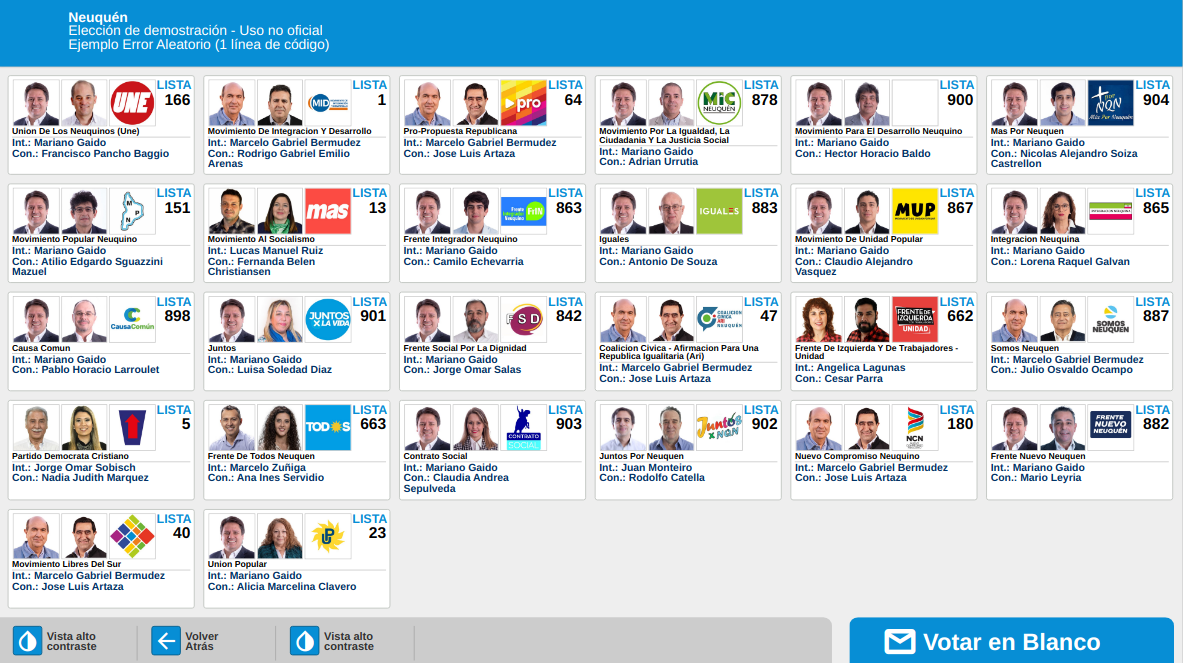
\includegraphics[width=\textwidth]{img/buenqn2019.png}
    \end{center}
  \caption{Pantalla del sistema BUE utilizado en las Elecciones Municipales de Neuquen 2019}
  \label{graf:buenqn}
\end{figure}

\subsection{Universalidad}
El sistema debe estar preparado para facilitar el sufragio de toda persona habilitada, esto incluye personas con requerimientos de accesibilidad, por ej. no videntes. Debemos tener en cuenta que toda persona posee los mismos derechos sobre el voto. Por lo tanto, si se requiere el acompañamiento debido a la complejidad o inaccesibilidad del sistema no se está alcanzando ninguna ventaja por sobre el sistema electoral tradicional.\newline
Como ejemplo, las máquinas usadas en elecciones electrónicas en general se basan en fotos y colores como medio de accesibilidad para las personas que no puedan leer o con baja visión. Por otro lado, en varios paises es común la instalación de un kit accesible como un teclado especial y auriculares para personas invidentes.

\subsection{Usabilidad}
%\cambiar{El sistema debe ser fácil y adecuado para toda persona involucrada en el proceso de la elección. Un sistema electrónico debe ser fácil de aprender tanto para un votante como para las autoridades encargadas de dar soporte. Esta propiedad también ayuda al objetivo de rapidez, ya que un sistema difícil de entender generará largas colas de espera para votar debido a que varias personas les lleva más tiempo entender y generar su sufragio. Así mismo la facilidad de uso mejoraría los tiempos del escrutinio realizado por las autoridades de mesa. - HECHO}

El sistema debe ser fácil e intuitivo para cualquier persona involucrada en el proceso de la elección. Un sistema electrónico debe ser fácil de aprender tanto para un votante como para las autoridades encargadas de dar soporte. Esta propiedad también ayuda al objetivo de rapidez ya que un sistema difícil de entender generará largas colas de espera para votar debido a que varias personas les lleva más tiempo entender y generar su sufragio. De igual manera la facilidad de uso mejoraría los tiempos del escrutinio realizado por cada autoridad de mesa.

\subsection{Cumplir con las normativas vigentes del proceso electoral}
Un sistema electoral regularmente no modifica sus políticas o reglas que lo conforman. De todos modos, un sistema de votación electrónica debe ser capaz de adaptarse a cualquier cambio adoptado por las autoridades de un país, provincia o distrito.

\subsection{Integridad vs. Auditabilidad vs. Secreto}
%\agregar{Agregar cita - HECHO}
En todo sistema electoral (sea en formato de papel o electrónico) se ha demostrado que satisfacer los atributos de integridad, auditabilidad y secreto simultáneamente es complejo y es una tarea imposible de cumplir. Cualquier sistema de voto electrónico que intente solucionar los problemas inherentes a garantizar integridad y secreto, estará en una situación difícil para lograr una verificación formal y en auditabilidad. \cite{conicet}

\section{Modelo de Referencia}
\cambiar{Sección 2.3: La Fig 2.2 presenta un circuito de 5 etapas para el proceso electoral. Debería nombrar en cada caso donde es aplicada la tecnología. Falta describir la etapa 5
(Procesamiento de resultados y publicación).}
\cambiar{Las subsecciones del modelo de referencia deben tener el mismo nombre. (Conteo →
Escrutinio de la Mesa)}
Mediante el análisis realizado por el Conicet \cite{conicet}, el sistema de votación se puede determinar en cinco fases secuenciales del proceso susceptibles de ser automatizada (Figura \ref{graf:modeloReferencia}) . Las fases están derivadas del Código Electoral Nacional (Decreto nº2135, 1983) \cite{decreto}
%\agregar{cita al Decreto}
%\agregar{artículo del CONICET - HECHO}

\begin{figure}[h!]
    \begin{center}
        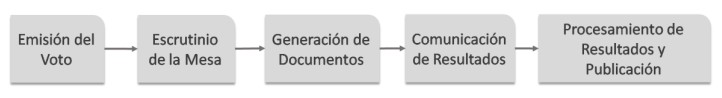
\includegraphics[width=\textwidth]{img/modeloReferencia.png}
    \end{center}
  \caption{Modelo de Referencia}
  \label{graf:modeloReferencia}
\end{figure}

%\agregar{Agregar imágen del modelo de referencia - HECHO}
%\cambiar{Está muy textual del artículo del CONICET (Modelo de Referencia, Comunicación de los resultados...., Conteo, Costo en tecnología),  Hay que parafrasear. Sacar la experiencia de los miembros de la Comisión - HECHO}
A continuación se analizan los riesgos y factibilidad técnica de las cuatro primeras fases del modelo de referencia teniendo en cuenta distintas fuentes de información, como son los atributos de calidad y antecedentes de otros países que se analizaron con anterioridad. 

%\cambiar{el orden de las subsecciones por el orden cronológico - HECHO:  el orden es por riesgo}
\subsection{Emisión del Voto} 
En la fase de Emisión del Voto, como su nombre indica, el votante expresa y registra su intención de voto. Cuando existe un dispositivo electrónico como intermediario entre el votante y su intención de voto se denomina al sistema como ``voto electrónico''. Esta fase incluye los atributos de calidad de universalidad del voto, igualdad de condiciones para la oferta electoral, integridad, secreto del voto y usabilidad descritas al comienzo del presente capítulo. Como se detalló anteriormente, la limitación técnica del ``voto electrónico'' es el requerimiento de mantener la confidencialidad del emisor del voto sin afectar la posibilidad de verificar si un voto fue emitido válidamente por un ciudadano habilitado o el voto registrado es consecuencia de un mal funcionamiento del sistema. Integrar tecnología en esta fase involucra un alto riesgo, un sistema distribuido de misión crítica es sumamente vulnerable a que una falla en un conjunto o todos los componentes que lo integran produzca un impacto general a todo el proceso electoral. Además una falla en esta fase (detectable o no) se puede propagar fácilmente a las siguientes fases del proceso electoral descritas en el modelo de referencia. 

Los riesgos que implica una máquina de emisión del voto a nivel de hardware son:
\begin{itemize}
    \item La máquina no está operativa.
    \item Manipulación para modificar la intención del voto.
    \item Manipulación en el guardado y/o transmisión de información adicional que permita posteriormente asociar al elector con su voto.
    \item Manipulación para alterar la representación de la oferta electoral.
    \item Se reemplazó por otro hardware no autorizado indistinguible por los usuarios.
\end{itemize}
%\cambiar{pk: y otros items descritos en articulo de Conicet ¿cuales? agregarlos o sacar la oración - HECHO}
Al ser una fase muy crítica esta máquina de emisión debe tener un diseño y construcción robusta para resistir manipulaciones maliciosas y vandalismo. Por lo tanto, existen ciertos requerimientos mínimos a nivel técnico del hardware como por ejemplo no debe tener almacenamiento estático (disco rígido, SSD, etc.), los componentes no deben ser accesibles salvo únicamente a través de la interfaz del usuario, para evitar comunicaciones PLC se debe filtrar toda conexión a la red eléctrica, es preferible el uso de baterías, no poseer memoria flash ni otro tipo de memoria no-volátil accesible en ejecución. \cite{conicet}

\subsection{Conteo} 
La fase de Conteo consiste en totalizar los datos por categoría y partido político. Este proceso necesita que cada autoridad de mesa realice el recuento independiente y auditado para finalizar en una o más actas con la misma información de la totalización. Incorporar tecnología en esta fase deberá ser para asistir en el conteo y que su resultado sea una primera aproximación. Sin embargo, el resultado final deberá ser plasmado en las actas con el dato obtenido por conteo manual y así cumplir el principio de independencia del software. 
Este conteo computarizado ayuda a las autoridades de mesa a aumentar su confianza en el resultado del conteo si coincide la cuenta manual con la cuenta electrónica, de todos modos se debe obligar a hacer el conteo manual y no colocar toda la confianza en la tecnología.
%\cambiar{, o sea, por ,es decir,}
Con respecto al hardware, la máquina encargada del conteo de votos tenemos los riesgos de que la máquina no se encuentre operativa o que sea manipulada para cambiar su comportamiento o que sea dañada completamente. Teniendo en cuenta estos problemas se debe tomar algunos recaudos a nivel hardware:
%\cambiar{pk: Agregar otros items....o bien resumirlos en una oración - HECHO}
    \begin{itemize}
        \item No poseer comunicación cableada o inalámbrica accesibles externamente.
        \item Preferiblemente usar baterías para evitar posibles comunicaciones PLC a través de la conexión a la red eléctrica.
        \item Mecanismos de seguridad evitando toda descarga de datos no autorizada.
        \item Separación física entre memoria de datos y memoria de instrucciones de proceso.
        \item Evitar cualquier intercambio de componentes al utilizar algún material con fuerte adherencia.
        \item Inmunidad a un ataque electromagnético moderado.
    \end{itemize}
    
\subsection{Generación de Documentos} 
La fase de Generación de Documentos inicia al momento que se dispone con el resultado del escrutinio de la mesa y finaliza con las actas, certificados y telegramas de escrutinio, todos estos firmados por las autoridades de mesa. En esta etapa es viable incorporar tecnología ya que puede mejorar el desempeño de la generación de estos documentos y en la verificación por parte de los partidos políticos. 
Sin embargo, puede afectar a la integridad de los documentos, los formatos impresos pueden no coincidir con los datos digitales y su detección puede ocurrir luego que se publicaron los resultados provisorios de la mesa. Este riesgo no es fácil de evitar aunque no afectaría al resultado del escrutinio definitivo. 
Con respecto al hardware, es decir la máquina encargada de generar los documentos puede presentar problemas como no estar operativa, no puede generar o imprimir los documentos o no puede enviar los documentos electrónicos. Otro de los problemas que puede incorporar es la alteración de los documentos electrónicos en tránsito.

Como se puede ver, los riesgos están relacionados al mecanismo de transmisión, por lo tanto no requiere un control de seguridad tan estricto como las fases anteriores del modelo de referencia. Relacionado al aspecto técnico del hardware se debería considerar que la máquina no posea puertos de comunicación cableado o inalámbricos accesibles externamente y debería existir una separación física entre la memoria de datos y la memoria de instrucciones de proceso. 

\subsection{Comunicación de Resultados} 
La fase de Comunicación de Resultados implica la transmisión de datos desde el lugar de votación hacia el centro de cómputos. Sabiendo que en un sistema de votación cada autoridad de mesa cuenta con un telegrama de escrutinio firmado correspondiente a su mesa, por lo tanto, reducir demoras en la transmisión de estos telegramas es viable realizar su digitalización y transmisión desde el mismo lugar de votación. Un ejemplo a esta situación fue el sistema usado en las PASO el año 2019 en Argentina, este sistema digitalizó y transmitió este telegrama completado y firmado por los representantes de la mesa correspondiente \footnote{https://www.infobae.com/politica/2019/07/20/como-es-el-nuevo-sistema-de-transmision-de-datos-que-debutara-en-las-paso/}.
%\agregar{año de la elección 2019, y alguna cita que mencione el proceso puede ser una noticia - HECHO} 
Esta transmisión incrementa las propiedades de confiabilidad y verificabilidad del sistema si se transmite tanto la imagen del telegrama como la información contenida. De tal manera, cualquier ciudadano podrá contrastar la información digital con la imagen del telegrama y poder así determinar si existen inconsistencias entre lo impreso y lo digital.

Contar con un soporte digital del telegrama evita la carga centralizada y manual de los datos en el centro de procesamiento. Otra ventaja de contar con la imagen del telegrama y la información digital es que el resultado de la mesa se podría publicar directamente sin necesidad de ninguna intervención humana. Por supuesto, esta situación ideal requiere una evaluación más cuidadosa, ya que está en juego la integridad de los datos, por lo tanto, si esta integridad fue manipulada y los datos digitales no coinciden con lo impreso o cualquier otra situación anómala (por ejemplo la falta de firmas en el telegrama, o números impresos difíciles de distinguir) pondrá en duda la confiabilidad del sistema. Como alternativa a esta situación es útil incorporar un proceso de validación de los datos.


\section{Costo en tecnología}
Uno de los principales factores para la selección de la tecnología a utilizar es la inversión necesaria. Para el caso del hardware usado para procesos de votación, el uso es relativamente bajo pero se encuentra justificada en función del impacto y seguridad del proceso. A esto debe sumarse el costo del depósito, traslado y custodia. \newline
%\cambiar{El sistema usado para las elecciones provinciales en Neuquén para 2019 costó mas de 100 millones de pesos, brindado por la empresa MSA ganadora de la licitación. Este costo incluye capacitación del personal interviniente.\cite{eleccionesNeuquen} - HECHO}
El sistema usado para las elecciones provinciales en Neuquén para 2019 costó más de 100 millones de pesos, brindado por la empresa MSA \footnote{https://www.msa.com.ar/} ganadora de la licitación. Esta inversión incluyó custodia, traslado, hardware y capacitación del personal técnico.\cite{eleccionesNeuquen}

\section{Conclusión}
\cambiar{La conclusión no tiene relación con lo realizado en el capítulo. Habla de Gukena. ¿Qué es Gukena? Nunca fue nombrado en este capítulo.}
Tomando este modelo de referencia podemos decir que Gukena es un sistema que se involucró en las etapas menos críticas o si ocurre algún error queda en evidencia y se puede corregir al instante. Estas etapas son: 
\begin{itemize}
    \item Conteo: sólo como ayuda para verificar datos finales, como por ejemplo la cantidad de votantes no debe superar la cantidad de empadronados en una mesa particular.
    \item Comunicación de Resultados: transmite los datos cargados hacia los servidores internos del sistema.
    \item Procesamiento de Resultados y Publicación.
\end{itemize}
De esta manera Gukena no se involucra en las etapas cercanas al voto individual obligando a que el escrutinio de una mesa sea manual, y que el acta sea en papel (etapa Generación de Documentos) firmado por todas las autoridades de la mesa.
%\agregar{Agregar una Sección de Conclusiones del Capítulo del porqué gukena solo agrega tecnología a la última etapa - HECHO}
\label{Elecciones}
\chapter{Análisis Elecciones}
%\agregar{Introducción al Capítulo y Descripción de las secciones - HECHO}

Un sistema de votación exitoso debe cumplir el principal objetivo que es construir la confianza de toda persona involucrada en el proceso: ciudadanos, partidos políticos, gobierno, entre otros. Como posibles alternativas en este proceso, planteadas a nivel mundial, ha sido aplicar distintas técnicas para computarizar parte del proceso de votación. 
Experiencias de implementación de voto electrónico en distintos países obtuvieron impactos de aceptación o con unos cuantos intentos volvieron al sistema electoral tradicional.

\section{Elecciones Internacionales}
%\agregar{Descripción de la seccion - HECHO}
A continuación se eligieron algunos países que implementaron tecnología dentro del proceso de votación. Además se describe brevemente las consecuencias obtenidas y la decisión de cada gobierno en continuar o no utilizando esta técnica.

\subsection{EEUU}
En los años 50 y 60 se utilizaron boletas de tarjetas perforadas, pero este sistema generó mayores problemas al momento del escrutinio como por ejemplo, abolladuras en el papel, se consideraban válidas las marcas sólo si todos los presentes estaban de acuerdo. Las papeletas marcadas con pluma, perforadas más de una vez, perforadas de forma ambigua (por ejemplo, en la línea entre dos partidos) o sin perforación se consideraban votos inválidos.
Como solución a los problemas evidentes de los sistemas de tarjetas perforadas, comienza el auge de los dispositivos de registro electrónico directo de votos (DRE). El uso de dispositivos de votación en EEUU cobró especial relevancia a partir del año 2000, luego de las elecciones presidenciales en donde un gran número de votos no fueron registrados apropiadamente.  \newline
Actualmente, en los distintos estados se emplean diferentes sistemas, que a menudo son utilizados de forma combinada.
%\cambiar{Sin embargo, existen debates sobre los dispositivos utilizados, y han habido causas judiciales en muchos estados respecto a su uso - HECHO}
Sin embargo, existen debates sobre los dispositivos utilizados, y hubo causas judiciales en muchos estados respecto a su uso. Como ejemplo en el estado de Pensilvania se produjeron varios problemas en el equipo de votación electrónica utilizados en Noviembre del 2019, generando suficiente desconfianza en el sistema de votación para las elecciones del 2020. Otro caso es el ocurrido en Nueva Jersey en el que los resultados fueron inmediatos pero el total de votos emitidos no coincidía con la suma de los votos emitidos por partido \cite{eleccionesEEUU}.
En 2002 se aprueba la ley federal Help America Vote Act., que establece un organismo de control denominado Eleccion Assistance Commission (EAC). El EAC conforma un comité técnico para delinear recomendaciones guías para los sistemas de votación, en aspectos de seguridad, testing de usabilidad y establecimiento de estándares y método de prueba para sistemas de votación electrónica. En 2007, la EAC comenzó el proceso de certificación de equipamiento de voto electrónico. Además esta comisión lleva registro de distintos problemas reportados sobre los dispositivos que se usan en la actualidad (Voting System Reports Collecction, 2017) \cite{problemasReportados}.

\subsection{Irlanda}
La primera propuesta de voto electrónico en Irlanda se realizó en 1998 y en el 2000 se introdujo la legislación que permitió el voto eletrónico. Para el 2002, se hicieron las primeras pruebas piloto con el objetivo de extenderlo al resto del pais. Pasaron unos meses para que un informe confidencial del Ministerio del Interior irlandés se filtrara a la prensa: allí se aseguraba que la integridad del proceso electoral no estaba garantizada. Entre otras fallas, el memorando interno que tomó estado público destacaba la posibilidad de que un software malicioso sencillo de programar pudiera generar una pantalla falsa en la máquina para hacer votar incorrectamente al elector. A pesar de este manto de sospecha sobre el sistema, el gobierno irlandés avanzó con el plan de implementación para las eleciones locales y europeas de 2004. Entonces creó la Comisión Independiente de Votación y Escrutinio Eletrónico para que examinara el sistema propuesto. La comisión emitió un informe en el que sostuvo que puede recomendar la utilización del sistema de voto eletrónico pero que, no podía garantizar la seguridad del voto y la rigurosidad del escrutinio. El gobierno no dio marcha atrás con el sistema pero lo puso en suspenso. La inversión que hizo Irlanda en el sistema fue uno de los argumentos principales de las autoridades para no descartar el sistema. Como resultado se registró 52 millones de libras iniciales que se le pagaron a Nedap, y se agregaban los costos de mantenimiento y de actualizacion del sistema (calculando en 700.000 euros anuales y 20.000.000 por única vez).\newline
Finalmente, el 23 de abril de 2009 el entonces ministro anunció que quedaba descartado el sistema de voto electrónico, en base al alto costo de mantenimiento y actualización, sumado a la insatisfacción y sospechas que generó entre los electores. En 2019 se realizó una encuesta al público sobre el uso de elecciones electrónicas consiguiendo un 50\% de aceptación. \cite{eleccionesIrlanda}
\subsection{Holanda}
En el 2008 (un año antes que en el caso irlandés) el gobierno de Holanda había tomado la misma decisión: abandonar el sistema de voto electrónico que había comprado a una empresa local, Nedap. La batalla contra el voto eletrónico en Holanda fue un grupo de activistas informáticos denominado "We don't trust voting computers". Este grupo además de presentaciones judiciales, realizaron una demostración pública en un programa de televisión de las múltiples formas en las que se podía acceder y tomar el control de las máquinas Nedap sin demasiado esfuerzo. En menos de cinco minutos, lograron correr su propio software en una máquina de la empresa y repartir votos de acuerdo a sus preferencias, engañando al elector que utilizaba la máquina. Hasta el día de hoy, Holanda mantiene el sistema de voto por medio de boleta de papel.\cite{netherlands}

%\agregar{citar fuente sumado  artículos científicos por scholar por ejemplo https://ieeexplore.ieee.org/abstract/document/7001135 - HECHO}
\subsection{Estonia}
En las elecciones municipales del 2005, Estonia se convirtió en el primer país del mundo en probar el voto por Internet, remoto. El sistema permite optativamente votar por Internet desde un lugar remoto, la identificación se hace a través del documento nacional de identidad que es una tarjeta inteligente; el voto por Internet es previo al día de la votación dejando al elector modificar su voto las veces que desee, tomándose como válido el último voto. En 2005, casi el 2\% utilizó el mecanismo de voto por Internet y fue creciendo hasta llegar al 30\% de la población en 2015. Las pocas garantías que ofrece sobre el carácter secreto del voto es una de las principales críticas que recibe este sistema. Los expertos consideraron que se debía suspender la aplicación de esta forma de votación, pero las quejas fueron rechazadas por el Comité de Voto por Internet del país y, en 2015, Estonia celebró sus elecciones con el sistema de voto por Internet.\cite{vassil2016diffusion}

%\agregar{citar fuente sumado  artículos científicos scholar - HECHO}

\subsection{Alemania}
A partir de 1998 comenzó a utilizar dispositivos electrónicos de voto (DRE Nedap utilizados en Holanda), comenzando con pruebas pilotos en Colonia y sucesivamente adoptados en distintas ciudades, y generalmente bien aceptadas por la ciudadanía, hasta 2005. En ese año, un par de ciudadanos presentaron una causa ante la Corte Constitucional Alemana, alegando que el uso de máquinas de votación electrónica es inconstitucional y que, dado que son vulnerables, los resultados de las presidenciales de 2005 no son confiables. Un fallo de esta corte dictaminó que el uso de las máquinas Nedap es inconstitucional, aunque no prohíbe el uso de cualquier dispositivo electrónico, sino que requiere que los mismos sean transparentes. Hoy Alemania usa la boleta única en papel.\cite{volkamer2010electronic}

%\agregar{citar fuente sumado  artículos científicos scholar - HECHO %? \url{http://www.brunazo.eng.br/voto-e/textos/CIPPEC-Brunazo.htm}
%\url{http://www2.congreso.gob.pe/sicr/cendocbib/con2_uibd.nsf/1B5274E790C782A1052577BB0075538C/\$FILE/El\_Voto\_Electr\%C3\%B3nico_en_Brasil.pdf}}
\subsection{Brasil}
En 2002 implementó una elección a escala nacional utilizando unos 406.000 dispositivos electrónicos (DRE) en la cual más de 100 millones de votantes emitieron su sufragio. Los reportes de testing de seguridad públicos en 2012 muestran que existen problemas técnicos severos en los dispositivos utilizados. Entre los problemas más relevantes se señalan la inadecuada protección del secreto del voto, el uso inapropiado de encriptación y algoritmos de criptografía obsoletos, modelos de ataques inadecuados centrados en atacantes externos cuando los ataques internos presentan un riesgo mucho mayor, adopción de un proceso de desarrollo de software defectuoso y verificación de integridad insuficiente.\cite{brunazo2005voto}

%\agregar{Sección Experiencias en Argentina y como Subsecciones cada una de las experiencias - HECHO}
\section{Experiencias en Argentina}
%\agregar{En el país hay experiencias de sumar tecnología en Elecciones Municipales, Provinciales y Nacionales, con diferentes niveles de aceptación, metodologías y aplicado a distintas fases del proceso.  En algunas implementaciones solo se agrega tecnología a la fase de Comunicación de Resultados y en otros a todo el procesos desde la fase de Emisión del voto.....  En las siguientes sub-secciones se describen algunas experiencias a nivel Municipal, Provincial y Nacional - HECHO}
Además de las experiencias de implementación de voto electrónico en distintos países con variadas técnicas, tenemos ejemplos a nivel nacional en Elecciones Municipales, Provinciales y Nacionales. Estas experiencias tuvieron diferentes niveles de aceptación, metodologías y distintas fases del proceso de votación involucraron tecnología. En las siguientes subsecciones se describen ejemplos de experiencias en Argentina.

%\cambiar{Elecciones Municipalidad de Las Grutas - HECHO}
\subsection{Elección Municipal de Las Grutas}
El 16 de diciembre de 2007 se utilizaron 4 urnas electrónicas de la firma Altec Sociedad del Estado (Rio Negro) en la localidad de Las Grutas (Argentina). Durante la jornada electoral, ocurrieron casos donde la urna no habilitaba al votante siendo que en el padrón en papel figuraba, siendo un claro atentado contra el secreto del voto. Otro de los problemas fueron máquinas que se trababan y al trabarse el papel utilizado dejaba en evidencia la elección del votante. La utilización de estas urnas electrónicas se implementó a pesar que el 10\% de los habitantes del lugar elevaran al superior tribunal de justicia la no obligatoriedad de este sistema. \cite{eleccionesLasGrutas}
%\cambiar{Elecciones Provinciales Neuquén - HECHO}
\subsection{Elecciones Provinciales de Neuquén en 2019}
El 10 de Marzo de 2019, Neuquén realizó la elección para gobernador y vicegobernador por medio del sistema de boleta electrónica, y con el sistema tradicional en papel en mesas con menor concurrencia. Se utilizaron máquinas BUE como se muestra en la figura \ref{fig:maquinasBUE}, las cuales eran manipuladas directamente por el votante, imprimiendo su votación sobre una boleta electrónica utilizando un chip que luego es usado para el escrutinio de cada mesa. El proceso de votación se conformó de las características en el proceso:
%\cambiar{y con el sistema tradicional en papel solo ....\% \url{http://200.70.33.130/images2/Electoral/CP_10-03-2019/Info_general/datos_generales_de_la_eleccion.pdf} - HECHO}
\begin{figure}
\begin{center}
  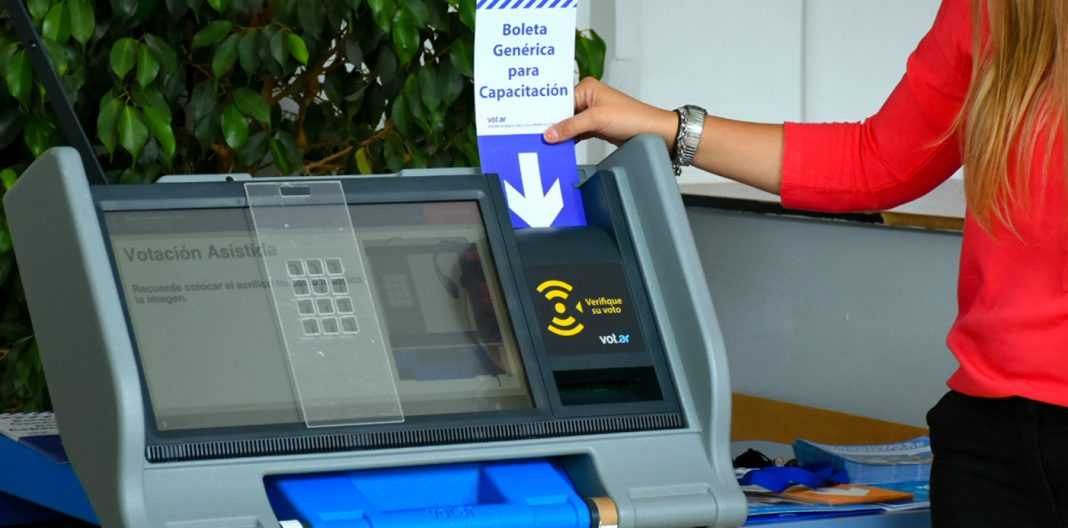
\includegraphics[scale=0.4]{img/Maquina_BUE.jpg}
  \caption{Máquina utilizada en las elecciones de Neuquén}
  \label{fig:maquinasBUE}
\end{center}
\end{figure}
\begin{itemize}
    \item Votación utilizando la máquina electrónica.
    \item Conteo utilizando la maquina electrónica y las boletas electrónicas.
    \item Envío de datos de las escuelas con la máquina electrónica utilizando el certificado generado de cada escrutinio de la mesa.
    \item Resultados provisorios
\end{itemize}

\newline Sobre estas elecciones se obtuvieron los siguientes datos \footnote{http://200.70.33.130/images2/Electoral/CP_10-03-2019/Info\_general/datos\_generales\_de\_la\_eleccion.pdf}:
\begin{itemize}
    \item 493.760 neuquinos estuvieron habilitados para votar, de los cuales se contabilizó una participación del 78.44%
    \item 1.504 mesas distribuidas en 283 escuelas, de las cuales 191 trabajaron con el sistema BUE (Boleta Única Electrónica), 86 con el sistema tradicional de papel y 6 escuelas tuvieron ambos sistemas
\end{itemize}

Se obtuvieron los datos de estas elecciones utilizando la técnica de Web Data Scraping, esta técnica se basa en un proceso de extracción y combinación de contenido alojado en la Web de manera sistemática. Se extraen los datos de interés y se lo estructura como se lo desee \cite{glez2014web}.

Para aplicar esta técnica se utilizó un pequeño script para extraer y estructurar la información obtenida a través de una API, provista por la provincia de Neuquén, hacia una estructura útil para nuestro propósito. Se analizaron los datos y se puede ver la evolución de la carga de mesas en el gráfico \ref{graf:porcentajeNeuquen} y su velocidad de carga en el gráfico \ref{graf:velocidadNeuquen}. Como se puede ver, los datos fueron agrupados en fracciones de 10 min durante todo el proceso de escrutinio.

\begin{figure}[h!]
  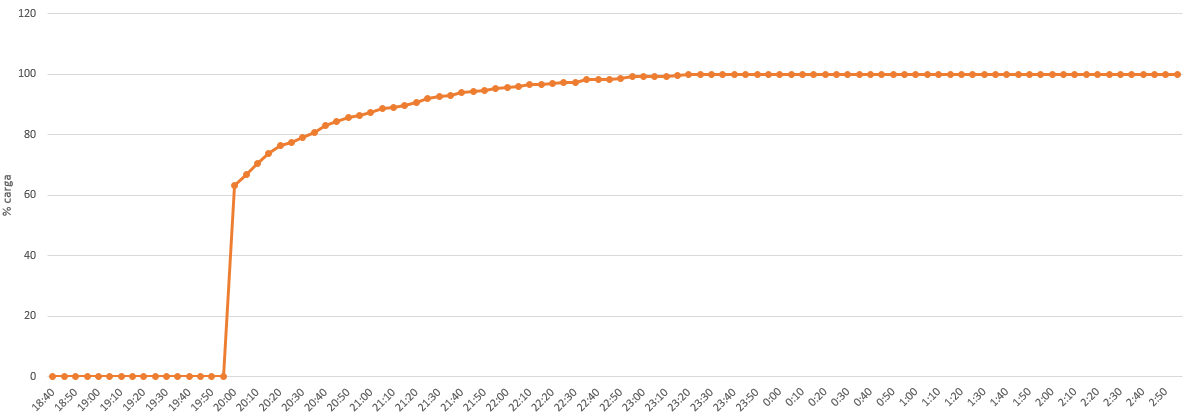
\includegraphics[width=1\textwidth]{img/fOI0sHj9ac.png}
  \caption{Porcentaje de mesas cargadas - Neuquén (2019)}
  \label{graf:porcentajeNeuquen}
\end{figure}

\begin{figure}[h!]
  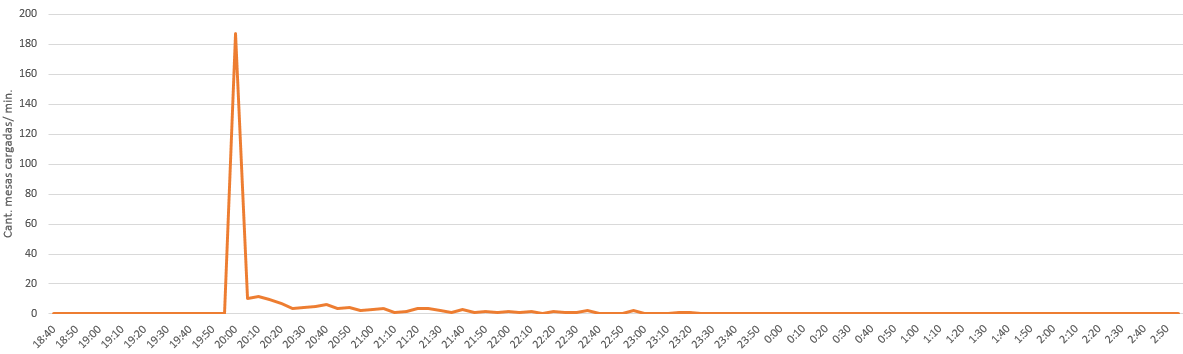
\includegraphics[width=1\textwidth]{img/QOsSnICbyL.png}
  \caption{Velocidad en carga de mesas - Neuquén (2019)}
  \label{graf:velocidadNeuquen}
\end{figure}


\subsection{Elecciones Provinciales de Rio Negro en 2019}
El 7 de Abril de 2019, Río Negro realizó la elección para gobernador y vicegobernador por medio del sistema tradicional de votación en papel. Cada votante contendrá en su sobre su lista y/o listas elegida en papel y, el escrutinio se realiza manualmente enviándose los datos desde cada escuela por medio de telegramas. El proceso de votación para esta elección se conformó de los siguientes elementos:
\begin{itemize}
    \item 7 listas candidatas que el elector puede elegir.
    \item 546.067 electores habilitados, esto quiere decir que se prepararon 546.000 sobres aproximadamante, uno por cada elector.
    \item 1646 mesas, esto implica la misma cantidad de urnas.
\end{itemize}
Teniendo estos datos se puede concluir que sólo para elecciones de gobernador y vice se utilizaron aprox. 3.822.000 papeles, 7 listas preparadas para 546.000 electores. De igual manera que en las elecciones de Neuquén, se obtuvieron los datos de las elecciones utilizando la técnica de web scraping, obteniendo una evolución de carga de mesas representado en el gráfico \ref{graf:porcentajeRioNegro} y su velocidad de carga en el gráfico \ref{graf:velocidadRioNegro}. Como se puede ver, los datos fueron agrupados en fracciones de 10 min durante todo el proceso de escrutinio.

%\agregar{explicación de que se trata y cita a algún artículo científico - HECHO}

%\cambiar{Caption de \ref{graf:porcentajeRioNegro}  \ref{graf:velocidadRioNegro} las de Córdoba también aclarando de que elecciones es y de cuando es.   De neuquen no hay gráfico? - HECHO} 
\begin{figure}[h!]
  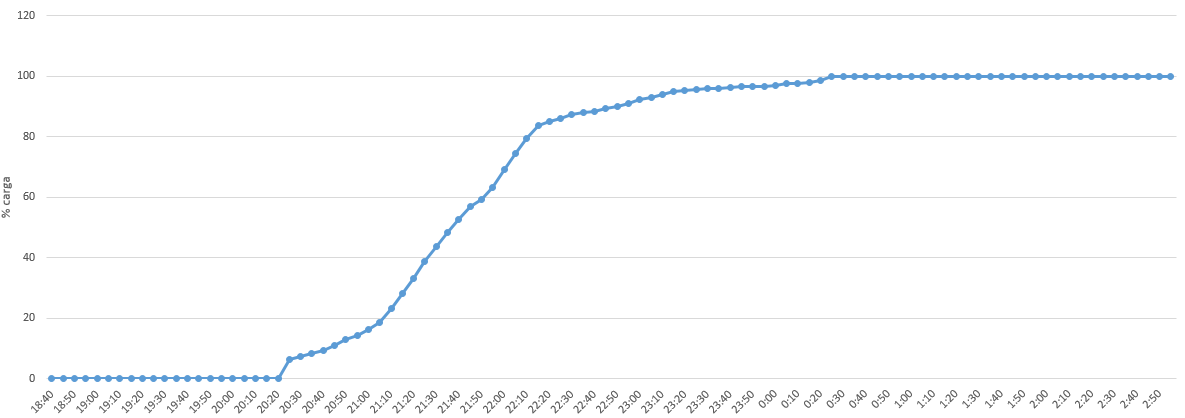
\includegraphics[width=1\textwidth]{img/sAveHlGEkX.png}
  \caption{Porcentaje de mesas cargadas - Rio Negro (2019)}
  \label{graf:porcentajeRioNegro}
\end{figure}

\begin{figure}[h!]
  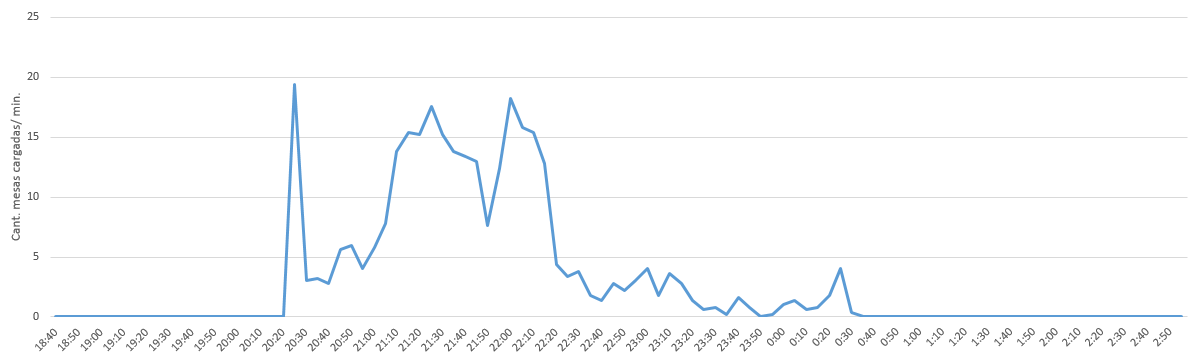
\includegraphics[width=1\textwidth]{img/8w25IVQD5U.png}
  \caption{Velocidad en carga de mesas - Rio Negro (2019)}
  \label{graf:velocidadRioNegro}
\end{figure}

\subsection{Elecciones Provinciales de Córdoba}
%\cambiar{No es boleta única papel? hay una impresora en cada mesa? - HECHO}
El 12 de Mayo de 2019, Córdoba realizó la elección para gobernador, legisladores,  candidatos a ocupar el tribunal de cuentas provincial, y en algunas localidades se renovaron autoridades municipales, por medio del sistema de boleta única de sufragio (BUS) \cite{cortiboleta}. Este método consta de una única boleta impresa con todos los cargos y candidatos sobre el cual el votante indica su elección dentro de esta boleta, el cual se ingresa en la urna. En las columnas se organizan cada uno de los cargos y en las filas se listan los espacios políticos como se puede ver en la imagen \ref{graf:BUSCordoba}.
\begin{figure}[h!]
  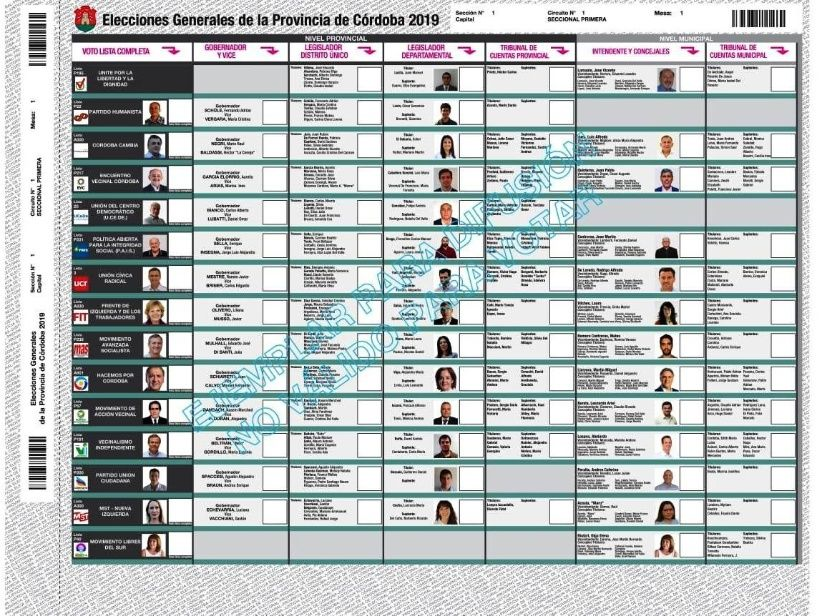
\includegraphics[width=1\textwidth]{img/boletaunica-cordoba.jpg}
  \caption{Ejemplo de la Boleta Única de Sufragio (BUS)}
  \label{graf:BUSCordoba}
\end{figure}
Luego el escrutinio se realizó de manera manual enviándose los datos de cada escuela por medio de telegramas. El proceso de votación para esta elección se conformó de los siguientes elementos: 
\begin{itemize}
    \item 13 listas candidatas para gobernador que el elector puede elegir
    \item 2.889.973 electores habilitados, esto quiere decir que se prepararon 2.889.000 boletas aproximadamente, uno por cada elector
    \item 8654 mesas
    \item 320 millones de pesos costó este sistema. 
\end{itemize}
%\cambiar{3.000.000 de boletas un poco más por las dudas. - HECHO}
Debido a que sólo se utiliza una boleta por elector, se puede concluir que sólo para elecciones de gobernador y vice se utilizaron cerca de 3.000.000 boletas en papel. Como se puede ver su resultado es mucho menor a las elecciones de Río Negro, aún teniendo éste cerca de un 20\% de electores habilitados a comparación de Córdoba. De igual manera que en las elecciones de Neuquén y Río Negro, se obtuvieron los datos de las elecciones utilizando la técnica de Web Data Scraping, obteniendo una evolución de carga de mesas representado en el gráfico \ref{graf:porcentajeCordoba} y su velocidad de carga en el gráfico \ref{graf:velocidadCordoba}. Como se puede ver, los datos agrupados en fracciones de 10 min. durante todo el proceso de escrutinio.

\begin{figure}[h!]
  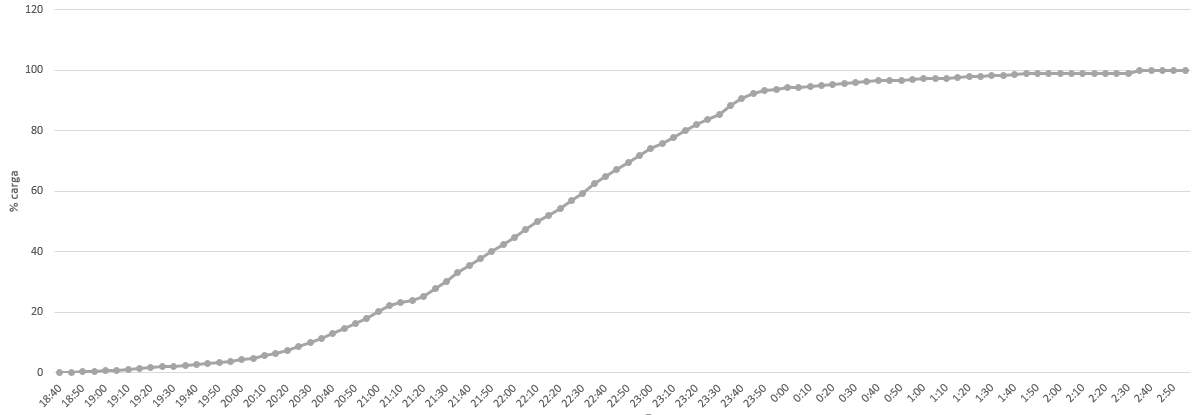
\includegraphics[width=1\textwidth]{img/E4YqKc5Tcu.png}
  \caption{Porcentaje de mesas cargadas - Córdoba (2019)}
  \label{graf:porcentajeCordoba}
\end{figure}

\begin{figure}[h!]
  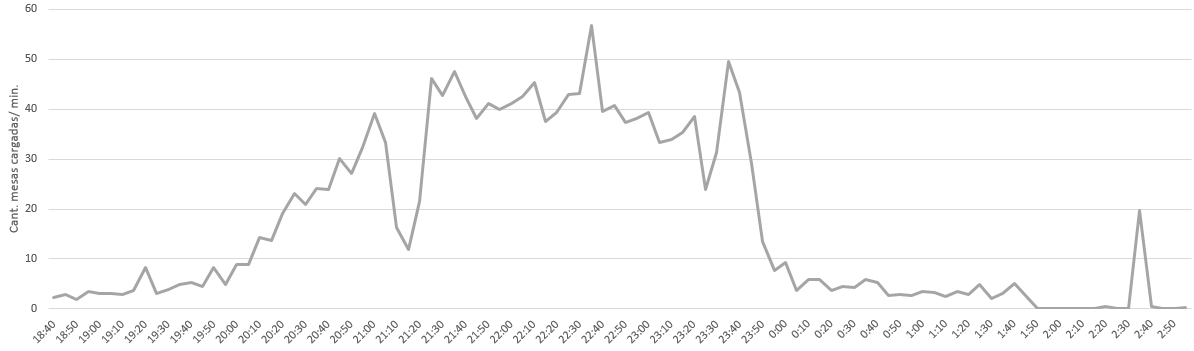
\includegraphics[width=1\textwidth]{img/9rEiyqeSFw.png}
  \caption{Velocidad en carga de mesas - Córdoba (2019)}
  \label{graf:velocidadCordoba}
\end{figure}

%\cambiar{llevaría esta sección como subsección de Experiencias en Argentina - ???}
\subsection{Sistema Escrutinio Nacional 2019}
En 2019 se utiliza el sistema llamado SmartTally \footnote{https://www.smartmatic.com/es/elecciones/elecciones-manuales/smarttally/}, que consta en el envío de telegramas directo desde el establecimiento hacia los centros de cómputos de la Dirección Nacional Electoral (DINE), que depende del Ministerio del Interior de la Nación. Con el objeto de agilizar el trámite que es llevado a cabo por el Correo Argentino. Cada establecimiento consta de una impresora multifunción, conexión a internet y un equipo que permite la conexión y monitoreo del envió exitoso de los telegramas. \newline
Este sistema fue usado en las elecciones las PASO (11 de Agosto de 2019) y Elecciones Naciones (27 de Octubre de 2019).
%\cambiar{Sacar la siguiente línea o bien describir el proceso - HECHO}

Polémicas al usar este tipo de sistema:
\begin{itemize}
    \item Auditabilidad del Software: Se requirió que la empresa ponga a disponibilidad el software usado para su investigación, a modo de reconocer posibles fallas. Frente a este pedido el Gobierno notifica que no es posible ya que el software es alquilado y la empresa dueña se niega a entregar este producto.\cite{auditabilidadSmartmatic}
    \item Seguridad frente a ataques externos: Javier Smaldone presentó vulnerabilidades en el software de conversión de formato de los ``telegramas'' electorales poniendo en riesgo la integridad del proceso. \cite{seguridadSmartmatic}
    \item Transparencia: Debido a que este sistema consta de dos etapas en el proceso de escrutinio, existe cierta desconfianza entre los datos cargados por cada transmisión exponiendo los resultados provisorios y el resultado final luego de ser validado dentro de los 10 días como indica el código electoral. Este primer resultado podría generar datos ganadores que luego no son así en el resultado final. \cite{rnEscrutinioProvisorio}
\end{itemize}



%\agregar{Sección Análisis de la utilización del Tecnología en Elecciones - ??}
\section{Análisis de la utilización de Tecnología en Elecciones}
El año 2019 fue un año ideal para el análisis de sistemas electoral nacionales, se realizaron múltiples elecciones a nivel municipal, provincial y nacional. Además de las magnitudes en cada elección se implementaron distintas técnicas en el proceso de elección. Esto permitió tomar experiencias y realizar una comparación de velocidad de publicación de resultados. A continuación de describen las elecciones provinciales en Neuquén, Rio Negro y Córdoba cuyas elecciones utilizaron diferentes sistemas. Con respecto a la ciudad de Neuquén Capital se realizó una encuesta del nivel de aceptación, confianza y conocimiento del sistema BUE utilizado en tres ocasiones anteriores a este año, por lo tanto, existía un aprendizaje de la población.

%\agregar{Durante el año 2019 en el país se realizaron múltiples elecciones a nivel municipal, provincial y nacional, situación que ha sido favorable para comparar diferentes sistemas.   En las siguiente sub-secciones se realizan una comparación de la velocidad de publicación de resultados de elecciones provinciales utilizando diferentes sistemas y un análisis mediante encuesta del nivel de aceptación, confianza y conocimiento del sistema BUE utilizado en las elecciones Municipales de la Ciudad de Neuquén - HECHO}

%\cambiar{Análisis comparativo de la velocidad de publicación de Resultados de elecciones Provinciales en Neuquén, Córdoba y Río Negro - HECHO}
\subsection{Análisis comparativo en Elecciones Provinciales de Neuquén, Córdoba y Río Negro en 2019}
A través de resultados almacenados en \textit{datosoficiales.com} se consiguieron los datos de cada elección detallada en las secciones anteriores de Neuquén, Río Negro y Córdoba.   \newline
En estas tres experiencias, las provincias contrataron a la empresa MSA \footnote{MSA \url{https://www.msa.com.ar/}} utilizando distintas técnicas, esto es aplicando tecnología en diferentes fases y logrando los resultados como se muestra en la tabla \ref{tab:comparativa}.
%\agregar{En las tres experiencias, las Provincias contrataron a la empresa MSA \footnote{MSA \url{https://www.msa.com.ar/}} utilizando diferentes técnicas, aplicando tecnología en diferentes faces y logrando diferentes resultados como muestra la Tabla \ref{tab:comparativa}.}
\begin{table}[]
    \centering
    \begin{tabular}{c|c|c|c}
         Provincia & Neuquén& Río Negro & Córdoba   \\
         \hline
         Técnica utilizada& BUE & Tradicional & BUS \\
         \hline
         Electores& & & \\
         \hline
         Mesas& & & \\
         \hline
         Tecnología aplicada a& &Comunicación de Resultados & Comunicación de Resultados \\
         \hline
         *Computado el 80\% & & & \\
         \hline
    \end{tabular}
    \caption{Comparativa de diferentes métodos utilizados en elecciones provinciales de 2019}
    \label{tab:comparativa}
\end{table}


A partir de esto, en el gráfico \ref{fig:velocidad} se puede observar la velocidad comparativa de cada carga en las tres provincias, y en el gráfico \ref{fig:acumulado} se representa el porcentaje acumulado durante el periodo de escrutinio. En estos gráficos, la linea naranja representaría las elecciones utilizando BUE, la linea gris las elecciones utilizando Boleta Única y la linea azul es el resultado de las elecciones tradicionales con boletas partidarias de papel. \newline
A primera impresión se puede observar la notable velocidad de carga en la provincia de Neuquén en los primeros minutos de las 20:00 hs., satisfaciendo el objetivo de rapidez de las máquinas BUE. Sin embargo, se reduce su velocidad hasta completar la totalidad de las mesas. Por otro lado, la provincia de Córdoba, por medio de la Boleta Única logra una velocidad constante de carga hasta completar la totalidad de las mesas. Como se puede observar en el gráfico \ref{fig:acumulado} la completitud de las mesas escrutadas se logra con poca diferencia de horas, dando a notar que aplicando tecnología en cualquier etapa del escrutinio no genera un impacto notable en la velocidad de los resultados. 
Al igual que estas elecciones sobre estas provincias, se intentó aplicar la técnica de Web Data Scraping para evaluar la velocidad de carga en las elecciones nacionales PASO y Generales de 2019. Sin embargo, no se logró obtener datos útiles para nuestro propósito ya que estos datos no contenían fechas y horas de publicación de cada mesa. Igualmente, en las Elecciones Generales 2019 a las 21:00 hrs. se logró publicar un 80\% del total de mesas, lo que muestra una técnica con muy buenos tiempos de velocidad de publicación de resultados.
%\agregar{Se realizó el mismo proceso de scraping para evaluar la velocidad de carga de las elecciones nacionales PASO y Generales 2019, pero el sistema de publicación de resultados no ofrecía el la fecha y hora en que se publicó cada mesa.  Igualmente, la segunda vez que se utilizó el sistema en las Elecciones Generales 2019, a las 21:00 ya había un 80\% de las mesas publicadas lo que muestra un método con muy buenos tiempos de velocidad de publicación de resultados...... ???}
\newline


\begin{figure}[h!]
  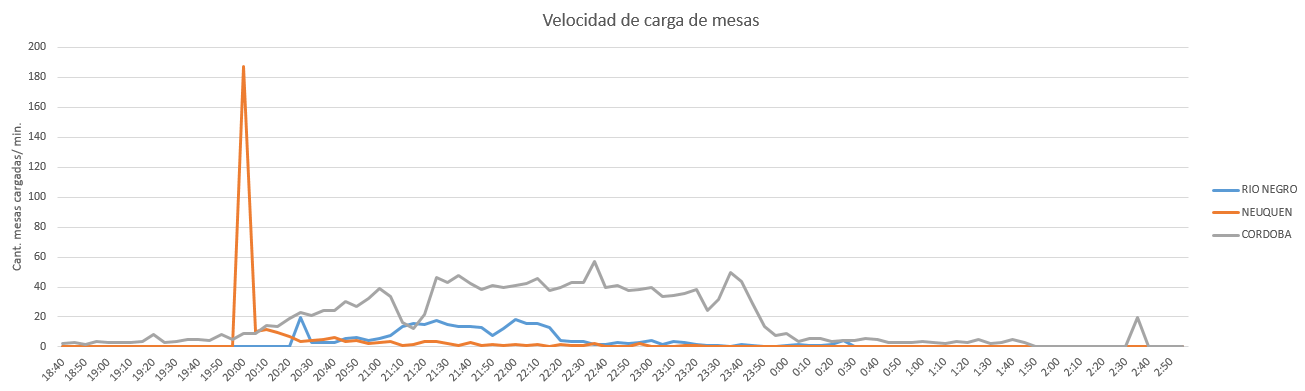
\includegraphics[width=\textwidth]{img/grafico_velocidad_carga.png}
  \caption{Velocidad de Cargas de mesas}
  \label{fig:velocidad}
\end{figure}
\begin{figure}[h!]
  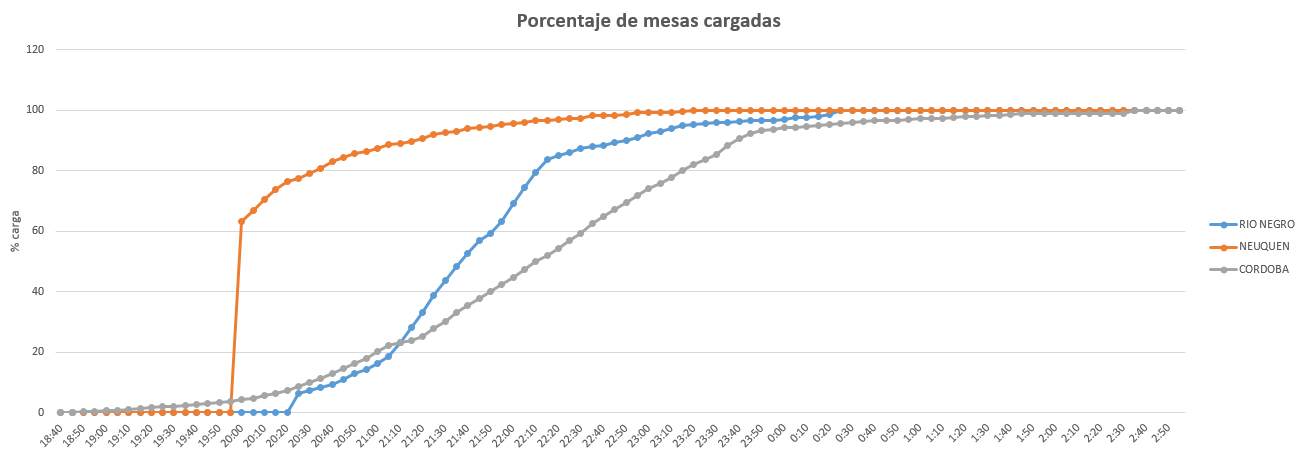
\includegraphics[width=\textwidth]{img/carga_mesas.png}
  \caption{Porcentaje de mesas cargadas}
  \label{fig:acumulado}
\end{figure}

Otra elección que logró implementar un sistema electoral tradicional sin intervención tecnólogica utilizando la boleta única fue en San Carlos de Bariloche el 1 de Septiembre del 2019 \footnote{Noticia: https://www.anbariloche.com.ar/noticias/2019/08/24/70978-elecciones-municipales-como-se-vota-con-la-boleta-unica}. Una característica que puede generar inconvenientes de este tipo de boleta es el tamaño que puede conseguir, ya que tiene que contener todas las listas disponibles. Por ejemplo, en las elecciones de Córdoba se tiene un tamaño de 40cm de alto por 47 cm de ancho como modelo general, este tamaño podría extenderse en municipios o dependiendo de la cantidad de partidos o alianzas que se presenten \cite{boletaUnicaTamanio}. \newline
Por otra parte, el sistema BUE consta de una boleta con un chif RFID sobre la cual se escribe la voluntad del votante. Dentro del modelo de referencia consta de las fases de Emisión del voto y además esta boleta es utilizada para la fase posterior de Escrutinio de la mesa. A pesar del debate impulsado por varias instituciones en contra del uso de este método, varios municipios lo utilizaron. Un inconveniente que puede albergar este sistema es la limitación en pantalla. Una pantalla dispone de 18 lugares para ubicar a los candidatos. Con el uso de listas colectoras se llegaron a multiplicar las listas. La disposición de los candidatos en la pantalla de estas máquinas puede afectar la accesibilidad de los electores al reducirse el tamaño de cada cuadricula. Como ejemplo, en Plottier \cite{lmncolectoras} se dispusieron 29 candidatos a intendencia de la ciudad y 26 en Neuquén. 
%\cambiar{Análisis de opinión pública sobre las elecciones en Neuquén Capital - HECHO}
\subsection{Análisis sobre la opinión pública sobre las elecciones en Neuquén Capital}
En las elecciones a intendente en Neuquén Capital el día 22 de Septiembre de 2019 se realizó una encuesta con la intención de conocer las opiniones de los votantes. Al ser un municipio que luego de 4 elecciones utilizando el sistema BUE, sería una buena muestra de votantes con experiencia sobre este dispositivo, o es lo que se espera. Esta actividad involucró votantes de cuatro escuelas repartidas en puntos importantes de la ciudad. Las escuelas encuestadas fueron Esc. nº201 (Barrio Centro), nº 40 (Barrio San Lorenzo), nº 20 (Barrio Don Bosco) y nº 103 (Barrio Confluencia) logrando encuestar 145 personas en total. \newline
El objetivo de esta encuesta fue conocer el nivel de aprendizaje de los votantes sobre este nuevo sistema y en respuesta a su uso, cuánta confianza y facilidad les resulta este medio de votación. A cada votante se le hacían cinco preguntas con opciones de respuesta para que el cuestionario se logre hacer en no más de 5 minutos. Las preguntas fueron:
\begin{enumerate}
    \item ¿La persona encuestada votó?
    \item ¿La persona encuestada leyó su boleta impresa?
    \item ¿La persona encuestada verificó su boleta utilizando el lector de chip RFID?
    \item ¿A la persona encuestada le resulta simple votar con la boleta BUE?
    \item ¿La persona encuestada confía en el sistema de votación utilizada?
\end{enumerate}

Cabe aclarar que esta encuesta se realizó a 100 metros de distancia de la escuela por Código Electoral y como se puede observar las preguntas estaban enfocadas a cómo realizar la votación, no se hicieron preguntas personales sobre su voto. Se decidió subdividir las muestras por edad generacional, por lo tanto, se encuadra cada votante dentro de las categorías
\begin{itemize}
    \item Z: Personas nacidas a partir del 2000, representado en la tabla como menores a 25 años aprox.
    \item Y: Personas nacidas entre 1980-1999, representado en la tabla con edades entre 25 y 39 años aprox.
    \item X: Personas nacidas entre 1965-1979, representado en la tabla con edades entre 39 y 55 años aprox.
    \item BG: Personas nacidas entre 1946-1964, representado en la tabla con edades mayores a 55 años aprox.
\end{itemize}
Al finalizar las encuestas se obtuvieron los datos de la tabla \ref{tab:encuesta} donde se contabilizan la cantidad de personas que respondieron a cada opción para cada pregunta.
\begin{table}[h!]
\caption{Resultado sobre los encuestados}
\begin{center}
\resizebox{\textwidth}{!}{
\begin{tabular}{ |c|c|||c|c|c||c|c|c||c|c|c||c|c|c|c| } 
 \hline
 \multirow{2}{4em}{Pregunta} & \multirow{2}{3em}{Generación} & \multicolumn{3}{|c||}{Escuela nº201} & \multicolumn{3}{|c||}{Escuela nº40} & \multicolumn{3}{|c||}{Escuela nº20} & \multicolumn{3}{|c|}{Escuela nº103} & \multirow{2}{3em}{Total}\\
  & &SI & MASO & NO & SI & MASO & NO & SI & MASO & NO & SI & MASO & NO & \\ 
 \hline
 \multirow{4}{3em}{¿Votó?} & Z < 25 & 2 & & & 7 & & & 4 & & & 5 & & & 18 \\ 
 & 25 <= Y < 39 & 8 & & & 12 & & & 12 & & & 4 & & & 36\\ 
 & 39 <= X < 55 & 15 & & & 12 & & & 13 & & & 23 & & & 63 \\
 & 55 <= BG & 12 & & & 5 & & & 7 & & & 4 & & & 28\\ 
 \hline \hline
 \multirow{4}{3em}{¿Leyó?} & Z < 25 & 1 & & 1 & 6 & & 1 & 4 & & & 5 & & & 18\\ 
 & 25 <= Y < 39 & 8 & & & 11 & & 1 & 11 & & 1 & 4 & & & 36\\ 
 & 39 <= X < 55 & 15 & & & 9 & & 3 & 11 & & 2 & 20 & & 3 & 63 \\
 & 55 <= BG & 11 & & 1 & 3 & & 2 & 7 & & & 3 & & 1 & 28 \\ 
 \hline \hline
 \multirow{4}{3em}{¿Verificó?} & Z < 25 &  & & 2 & 6 & & 1 & 1 & & 3 & 4 & & 1 & 18 \\ 
 & 25 <= Y < 39 & 5 & & 3 & 4 & & 7 & 8 & & 4 & 3 & & 1 & 36\\ 
 & 39 <= X < 55 & 8 & & 7 & 7 & & 6 & 4 & & 9 & 14 & & 9 & 63 \\
 & 55 <= BG & 5 & & 7 & 4 & & 1 & 4 & & 3 & 3 & & 1 & 28\\ 
 \hline \hline
 \multirow{4}{3em}{¿Es simple?} & Z < 25 & 2 & & & 6 & 1 & & 4 & & & 5 & & & 18 \\ 
 & 25 <= Y < 39 & 8 & & & 11 & & & 11 & 1 & & 4 & & & 35 \\ 
 & 39 <= X < 55 & 14 & & 1 & 12 & 1 & & 11 & 1 & 1 & 21 & 2 & & 64 \\
 & 55 <= BG & 12 & & & 3 & & 2 & 6 & & 1 & 2 & & 2 & 28 \\ 
 \hline \hline
 \multirow{4}{3em}{¿Confía?} & Z < 25 & 2 & & & 3 & & 4 & 1 & & 3 & 3 & 2 & & 18 \\ 
 & 25 <= Y < 39 & 4 & 3 & 1 & 1 & 4 & 6 & 6 & 1 & 5 & 1 & 1 & 2 & 33 \\ 
 & 39 <= X < 55 & 10 & 3 & 2 & 4 & 3 & 6 & 8 & 2 & 3 & 14 & 6 & 3 & 64\\
 & 55 <= BG & 10 & 2 & & & 1 & 4 & 3 & & 4 & 2 & & 2 & 28\\ 
 \hline \hline
\end{tabular}
}
\label{tab:encuesta}
\end{center}
\end{table}

Teniendo los datos finales, se logra ver una gran cantidad de personas que leen sus boletas impresas pero no asi con la lectura del chip integrado en la boleta, como se observa en el gráfico \ref{graf:votantes}. A pesar de haber experimentado este sistema en distintas elecciones se descubrió que muchos de ellos no sabian la existencia del lector de chip, dato que no se esperaba. Como se puede ver en el gráfico cerca del 50\% desconocía esta verificación y no varía según la edad generacional.

\begin{figure}[h!]
  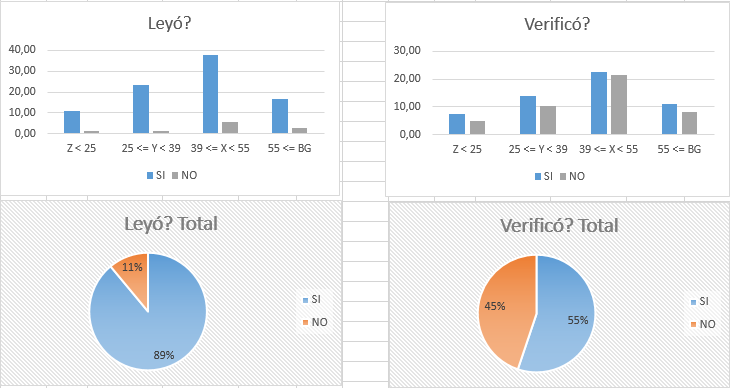
\includegraphics[width=\textwidth]{img/yfrjnCosp0.png}
  \caption{Comparación entre los que leen y verifican su boleta electrónica}
  \label{graf:votantes}
\end{figure}

Otro dato curioso de estas opiniones es que casi la totalidad de las personas les resulta sencillo su uso, sin embargo, muy pocas de ellas les genera confianza. Como se puede ver en el gráfico \ref{graf:votantesUsoConfia} la mitad de los encuestados les genera confianza o intentan confiar en este sistema. Sobre esta última característica destaca la variación de opiniones según la zona urbana encuestada, como se puede ver en la tabla \ref{tab:encuesta}, en el área centro (Escuela nº201)  se concentra la cantidad de personas que confían en sistema BUE, seguido del área Confluencia (Escuela nº40)  %\cambiar{Por otro lado las escuelas que se encuentran en zonas mas alejadas del centro no confían en este sistema. - HECHO}
Por otro lado las demás escuelas en zonas más alejadas del centro no logran confiar en este sistema. 
\begin{figure}[h!]
  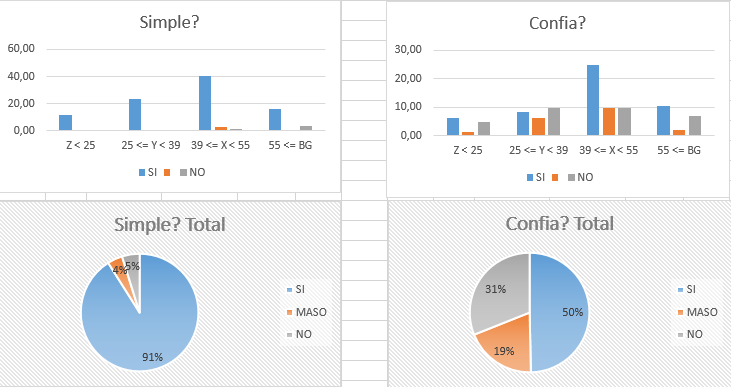
\includegraphics[width=\textwidth]{img/SLLXOorTia.png}
  \caption{Usabilidad vs. Confiabilidad}
  \label{graf:votantesUsoConfia}
\end{figure}


\label{Gukena}
\chapter{Gukena}
\cambiar{referencias mal citadas}
\cambiar{Si es cita textual se podría poner entre '' . \begin{quote}\textit{``Los usuarios exigen cualidades al software destinadas a facilitar su trabajo, ahorrar tiempo (de uso y de aprendizaje), evitar y corregir los errores''} \cite{definicionUsuarioInterfaz}\end{quote}}
Los usuarios exigen cualidades al software destinadas a facilitar su trabajo, ahorrar tiempo (de uso y de aprendizaje), evitar y corregir los errores \cite{definicionUsuarioInterfaz}. El cómputo provisorio de los votos en la Universidad Nacional del Comahue se realizaba en forma manual por una persona, encargada de ingresar los datos en una planilla electrónica. Esta persona era responsable de gestionar correctamente los resultados y distribuir los cargos. La forma de trabajo generaba un cuello de botella en la carga de los datos produciendo una demora de varias horas y hasta días en obtener los resultados finales.

Luego de haber analizado las propiedades sensibles que pueden ser afectadas al involucrar tecnología en alguna de las etapas dentro del proceso electoral, se desarrolla Gukena con la intención de ayudar y/o 
%\cambiar{acompañar al área responsable de realizar el cómputo de la elección.}
acompañar al área responsable de realizar el cómputo de las elecciones. Siempre dentro de las etapas sobre las cuales se corre menor riesgo de corromper la voluntad del votante. Gukena es un sistema responsable de realizar estos cómputos y distribuir la carga de trabajo hacia distintos sitios. Ha sido utilizado con éxito en las últimas elecciones que se desarrollaron en el ámbito de la Universidad Nacional del Comahue, usado a partir del año 2016. Este sistema ayuda a distribuir el trabajo en lo que respecta a la carga de la información de votos, y acorta el tiempo de espera para conocer los resultados provisorios de las elecciones, incluso permite observar resultados parciales en tiempo real.\newline

Una vez que la autoridad de mesa finaliza el recuento y completa el acta en papel,  la información es ingresada en el sistema manualmente desde cualquier computadora o dispositivo móvil con acceso a Internet. Previamente, las autoridades de mesa, recibieron un breve instructivo de carga y un sobre cerrado con usuario y clave para ingresar al sistema. De igual modo, además de esta carga electrónica, el acta en papel es enviada a la Junta Electoral. Con este soporte papel se resuelve cualquier inconveniente que pueda surgir, como la falta de acceso a Internet o cualquier otro,  impidiendo que el acta sea cargada por la autoridad de mesa, siendo la Junta Electoral quien se responsabiliza en realizar su carga al sistema.

Como segunda etapa, la junta electoral accede al sistema y verifica los datos cargados cotejando con las actas recibidas, permitiendo así resolver cualquier error de carga. 
El proceso de escrutinio finaliza con una última validación, sobre los datos de todas las mesas, a cargo de la secretaria de la Junta Electoral. 

Todo el proceso se encuentra disponible al público generando un ámbito transparente al presenciar y observar los resultados parciales en todo momento, tanto de manera presencial como virtual por medio de una página web abierta.

Algunas ventajas de utilizar el sistema, además de la disminución del tiempo en el proceso de escrutinio, son:
\begin{itemize}
\item Carga distribuida de las actas en el sistema, actas cargadas directamente por el responsable de la misma y sin intermediarios,
\item Resultados accesibles desde cualquier navegador o dispositivo con acceso a internet,
\item Ayudar a comprender mejor los datos de un acta mal redactada o poco legible,
\item Detectar consistencia en el recuento de votos. Contar con doble verificación permite detectar la totalidad de errores y validación de datos durante la carga del acta, ofreciendo mayor seguridad en esos momentos. Como por ejemplo, en casos en que se pretende registrar más votantes que la cantidad de empadronados que contiene la mesa.
\item Distribución de responsabilidades, tanto a nivel de carga de datos sobre distintos sitios, como distribución de roles dentro del sistema electoral como es la carga y validación.
\item Mejora en la visualización y búsqueda de datos cargados dentro del sistema, como ser por tipo de cargo o unidad académica, disponible a cualquier persona que acceda a la página de resultados.
\agregar{ Historial de elecciones pasadas disponible para consulta}

\end{itemize}

\section{Análisis}
\subsection{Metodología de desarrollo}
Utilizar una metodología adecuada al momento de un desarrollo es importante para lograr el objetivo del producto final. Existen muchas metodologías tradicionales y ágiles, estas últimas permiten un proceso de desarrollo más rápido con la intención de no afectar la calidad del producto. Una metodología ágil consiste en un desarrollo incremental con iteraciones muy cortas, beneficiando principalmente a proyectos con requisitos cambiantes y con exigencias en los tiempos
de desarrollo \cite{canos2012metodologias}. 
\cambiar{Volcando este concepto dentro del desarrollo de Gukena se utilizó una adaptación de la metodología SCRUM.}
Volcando este concepto dentro del desarrollo de Gukena se puede decir que se utilizó la metodología SCRUM. Cada año representa una iteración (o sprint), donde cada iteración duraba de 4-5 semanas de desarrollo con reuniones cada semana dentro de cada iteración. Las Historias de Usuario son las técnicas para especificar los requisitos del software, estas describen brevemente las características que el sistema debe poseer, requisitos funcionales o no funcionales.
\subsection{Historias de usuario en Gukena}
 Cada historia de usuario establecida en Gukena es comprensible y delimitada para que el equipo conformado pueda llevarla a cabo en unas semanas. A continuación se listan las historias de usuario que formaron parte de Gukena:
 \begin{enumerate}
     \item Armado de Carta Marina, precarga de datos y distribución de centros de votación
     \item ABM Acta de Junta Electoral
     \item Vista de resultados con login
     \item ABM Acta de Autoridad de Mesa
     \item Validación de actas de Junta Electoral
     \item Login de todos los usuarios y auditoría de sus acciones
     \item Resultados públicos
 \end{enumerate}
 
\subsection{Memorias del Desarrollo}
A través de los años Gukena sufrió una evolución en su funcionalidad y usabilidad, por esto a continuación se detallan cada uno de los items que formaron parte del desarrollo para satisfacer las historias de usuario.

\subsubsection{2015}

\begin{enumerate}
    
    \item Investigación y aprendizaje sobre el proceso y normativo de elecciones en la Uncoma y el uso del método D'Hondt.
    \item Diseño y modelado de la base de datos utilizando una base de datos relacional.
    \item Preparación del ambiente de trabajo, utilizando framework Toba y gestor de base de datos PostgreSQL.
    \item Creación de controladores para el formulario de carga de una Autoridad de Mesa.
    \item Creación de controladores para la grilla de mesas con sus estados.
    \item Creación de controladores para el resultado del escrutinio.
    \item Validación del sistema contra el archivo xls utilizado en el escrutinio oficial.
\end{enumerate}
\subsubsection{2016}
\begin{enumerate}
    \item Análisis y modelado de los datos involucrados en el control de acceso al sistema.
    \item Investigación e integración de seguridad utilizando la herramienta de login que provee el framework Toba
    \item Unión del modelado de datos referidos al control de acceso con la herramienta de login.
    \item Integración con registros de seguimiento sobre actualizaciones en los datos por parte de cada usuario logueado.
    \item Preparación de datos para las elecciones de este año.
    \item Testeo final sobre la funcionalidad en la carga de datos por Autoridades de mesa y su resultado final.
\end{enumerate}
\subsubsection{2017}
\begin{enumerate}
    \item Preparación de datos para las elecciones de este año (Carta marina).
    \item Testeo final sobre la funcionalidad en la carga de datos por Autoridades de mesa y su resultado final.
    \item Preparación del documento que especifica el Procedimiento de Gukena dentro del marco de elecciones en la UnComahue.
\end{enumerate}
\subsubsection{2018}
\begin{enumerate}
    \item Nuevo diseño y creación de pantallas accesibles por el público en general.
    \item Adaptación del sistema para crear archivos json con datos que serán consumidos por nuevas pantallas de Resultados.
    \item Creación de script encargado de copiar los archivos json entre dos servidores, desde el servidor procesador de los datos cargados por Autoridad de mesa y Junta electoral hacia el servidor público con la visualización de los resultados.
    \item Preparación del ambiente de trabajo, esto involucra ambos servidores junto al script y datos dentro del sistema(Carta marina).
    \item Testeo final sobre la funcionalidad en la carga de datos por Autoridades de mesa y su resultado final.
\end{enumerate}
\subsubsection{2019}
\begin{enumerate}
    \item Preparación del ambiente de trabajo, esto involucra ambos servidores junto al script y datos dentro del sistema(Carta marina).
    \item Testeo final sobre la funcionalidad en la carga de datos por Autoridades de mesa y su resultado final.
    \item Preparación del documento que especifica los datos accesibles públicamente en los archivos json.
\end{enumerate}

\section{Diseño}
\agregar{un párrafo que describe el concepto de diseño y una breve descripción de la Sección.}
\subsection{Arquitectura}
\begin{figure}[h!]
  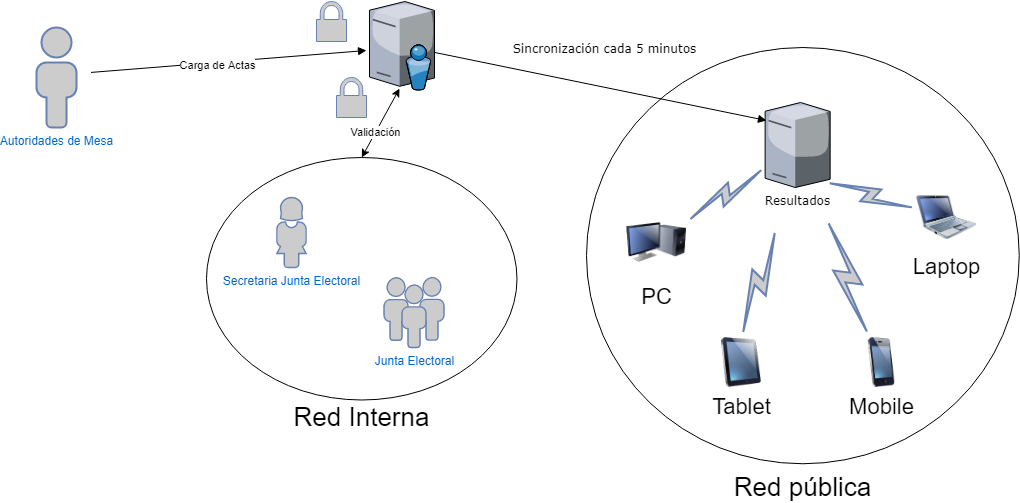
\includegraphics[width=\textwidth]{img/arquitectura.png}
  \caption{Arquitectura}
  \label{graf:arquitectura}
\end{figure}

Gukena se implementó sobre una arquitectura dividida en tres módulos (imagen \ref{graf:arquitectura}) que se relacionan con los diferentes roles que interaccionan con el sistema.
\begin{itemize}
\item Módulo Resultados: muestra los resultados en un servidor web público, para que la comunidad universitaria pueda conocer los resultados a medida que se van cargando los datos.
\item Módulo Autoridad de Mesa: desde cualquier dispositivo con conexión a Internet las Autoridades de Mesa acceden con su usuario y clave para cargar los datos del acta desde el lugar de votación.
\item Módulo Junta Electoral: los integrantes de la junta electoral y la Secretaria realizan un doble chequeo de las actas cargadas por las Autoridades de Mesa en una red interna.
\end{itemize}

La propiedad de usabilidad es importante para que un sistema sea fácil de aprender y de utilizar. Cada uno de estos módulos implican actividades disjuntas dentro del sistema, por lo tanto, para cada rol se le dispuso una interacción distinta con el sistema. \newline
El público en general tiene la necesidad de ver los resultados parciales durante el proceso de escrutinio, para cumplir este objetivo se accede a Gukena a través del sitio público de resultados \footnote{Sitio resultados: \url{https://resultados.uncoma.edu.ar}}.
Esta página es accesible desde cualquier navegador, contiene un historial de elecciones, categorías de búsqueda de información, gráficos y descripciones explicativas sobre los datos visualizados. Por otro lado, el rol de autoridad de mesa tiene la necesidad de transmitir la información del resultado de su escritinio, por este motivo acceden a sitio \footnote{Sitio Autoridades de Mesa y Junta Electoral: \url{https://gukena.fi.uncoma.edu.ar/}},
donde se loguean con la información recibida previamente y acceden a una única pantalla con un formulario correspondiente a la mesa escrutada. Por último tenemos al módulo de Junta Electoral quienes necesitan validar y/o corregir la información cargada en el sistema. Acceden al mismo link que una autoridad de mesa con la diferencia que al validar múltiples mesas, el sistema le dispone un listado de todas las mesas, con filtros y categorías para facilitar su búsqueda. Además, cada mesa se encuentra etiquetada con información sobre su estado, es decir, si ya fue cargada por la autoridad de mesa correspondiente o en la espera de su carga. Por cada mesa se le despliega la misma pantalla que se dispone a una autoridad de mesa para que pueda hacer las correcciones necesarias con una acción de validar esta información. Cabe destacar que una autoridad de mesa solo tiene disponible el formulario de carga hasta que envia la información cargada, a partir de ese momento solo puede visualizar el formulario pero no volver a editarlo.\newline

%\agregar{citaa LAMP - HECHO}
Por otro lado, a nivel técnico Gukena se desarrolló sobre una infraestructura web LAPP como variación a la arquitectura LAMP. Las siglas LAMP corresponde al paquete open source  \cite{chaparro2006lamp} que contiene: 
\begin{itemize}
    \item Linux: Sistema Operativo basado en software libre.
    \item Apache: Servidor web.
    \item MySQL: Servidor de base de datos relacionales open source.
    \item PHP: Lenguaje de programación open source embebido en páginas HTML, ejecutado en el servidor. Compatible con distintos sistemas operativos y bases de datos.
\end{itemize} Gukena se implementó sobre un sistema base Linux, servidor web Apache, el lenguaje de programación PHP y como variación utilizó el sistema gestor de base de datos PostgreSQL. 


\subsection{Modelo de datos}
 \cambiar{hablaría de entidades en vez de clases}

La semántica de este problema se representó sobre una base de datos relacional utilizando herramientas de software libre. Se utilizó el Gestor de Base de Datos PostgreSQL sobre un sistema operativo Linux. El modelo de datos representa los conceptos más importantes en un dominio, conociendo el proceso de elección en la Universidad Nacional del Comahue se puede ver que las clases más importantes son: unidad electoral, mesas, claustros, actas y las listas oficializadas para cada cargo. En base a estas clases principales tenemos los votos que recibe cada lista postulada que se agrupan por las sedes que conforman cada Unidad Electoral. Además para mantener el histórico de elecciones se tiene la clase de acto electoral manteniendo las fechas de cada elección realizada.\newline
Conociendo el modelo de datos, al momento de una nueva elección es necesario realizar una precarga de datos sobre:
\begin{itemize}
    \item Acto electoral con fecha de la nueva elección, asociando los claustros que votarán y las unidades electorales y sedes participantes
    \item Datos de las mesas: número de mesa, cantidad de empadronados en cada mesa, claustro al que pertenece.
    \item Listas oficializadas para cada claustro y el cargo al que se postula
    \item Usuarios habilitados a ingresar al sistema
\end{itemize}
%\cambiar{Diagrama del modelo de datos que representa las relaciones de la tablas en la Bases de Datos PostgreSQL - HECHO}
\begin{figure}[h!]
  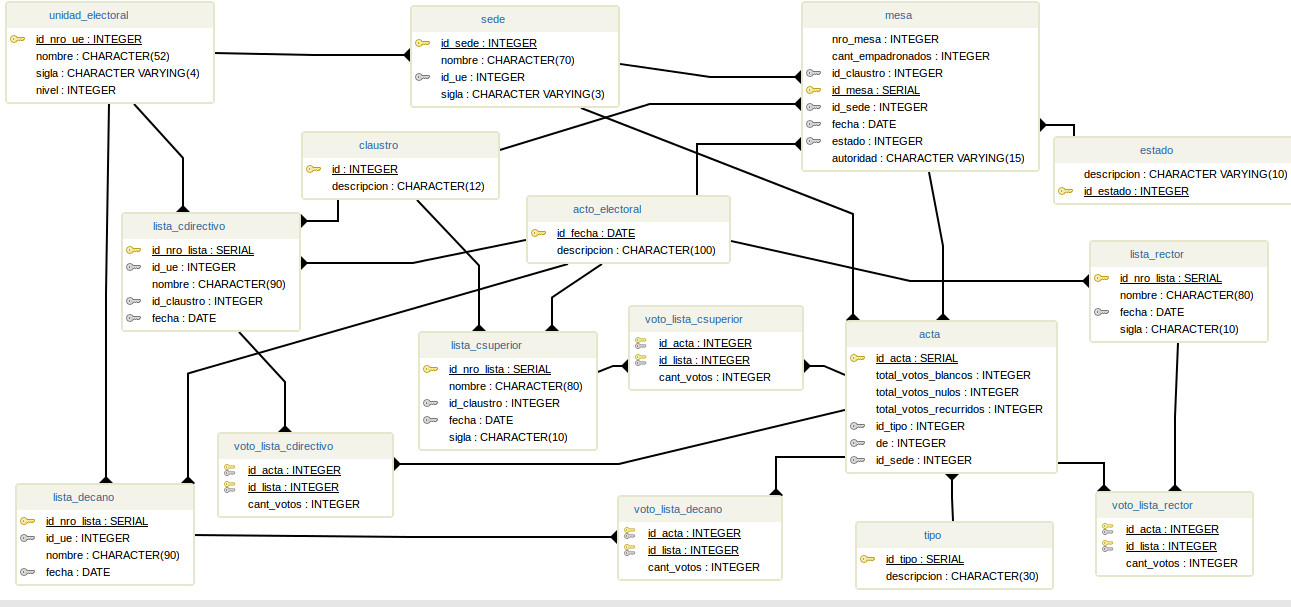
\includegraphics[width=\textwidth]{img/gu_kena_diagramaBD.jpg}
  \caption{Relación entre las tablas almacenadas en la Base de Datos Gukena}
  \label{graf:diagramaBD}
\end{figure}

Este modelo de datos representado en la Figura \ref{graf:diagramaBD} es el almacenamiento principal del sistema, es decir, la carga de datos por parte de las autoridades de mesa y Junta Electoral y, el procesamiento de los resultados impacta sobre esta fuente de datos. 

\subsection{Interoperabilidad externa}
\agregar{Agregar que se trata de una API REST.  Describir y citar que significa API REST. Poner un link real a modo de ejemplo }
La visualización de los resultados al público en general dispone de una segunda fuente de datos de Gukena conformada por archivos en formato JSON. Estos archivos son actualizados durante el escrutinio cada 5 minutos y son el resultado de procesar los datos existentes en la base de datos SQL. Estos archivos son consumidos por la página de Gukena pública, sin embargo, pueden ser consultados por cualquier sistema o persona que los quiera acceder. A continuación se describe brevemente la estructura y notación utilizada para un acceso externo a Gukena.
La estructura de estos archivos está formada por:
\begin{itemize}
    \item data (lista, sigla , total de votos, sede)
    \begin{itemize}
        \item lista (String)
        \item sigla (String)
        \item total de votos (int)
        \item sede (int)
    \end{itemize}
    \item columns (field , title)
    \begin{itemize}
        \item field (String)
        \item title (String)
    \end{itemize}
    \item titulo (String)
    \item labels (String)
    \item total (int)
    \item fecha (datetime)
    \item enviados y confirmadas (String)
    \item titulo\_grafico (String)
\end{itemize}
Para reconocer que archivo se debe consumir para obtener los datos deseados,  se aplicó una notación conformada por \textbf{nombreCargo} + \textbf{siglaUnidadElectoral} + \textbf{nombreClaustro} + \textbf{".json"} en el nombre de cada archivo. En la tabla \ref{tab:formatoJSON} se representa este formato.

\begin{table}[htbp]
\begin{center}
\begin{tabular}{|l|l|l|}
\hline
Categoria\_ & Unidad\_Electoral & \_ Claustro.json\\
\hline \hline 
R(Rector) & Todo(Universidad) & T(Total)\\ \hline
D(Decano) & ASMA & D(Docentes)\\ \hline
CD(Consejo Directivo) & AUZA & E(Estudiantes)\\ \hline
CS(Consejo Superior) & CRUB & G(Graduados)\\ \hline
-& CUZA & N(No Docentes) \\ \hline
-& ESCM &- \\ \hline
-& FACA &- \\ \hline
-& FACE &- \\ \hline
-& FADE &- \\ \hline
-& FACA &- \\ \hline
-& FAEA &- \\ \hline
-& FAHU &- \\ \hline
-& FAIF &- \\ \hline
-& FAIN &- \\ \hline
-& FALE &- \\ \hline
-& FAME &- \\ \hline
-& FATA &- \\ \hline
-& FATU &- \\ \hline
\end{tabular}
\end{center}
\caption{Nombre de archivos JSON}
\label{tab:formatoJSON}
\end{table}

\subsection{Seguridad}
Una vulnerabilidad (en términos de informática) es una debilidad o fallo en un sistema de información que pone en riesgo la seguridad de la información pudiendo permitir que un atacante pueda comprometer la integridad, disponibilidad o confidencialidad de la misma \cite{definicionVulnerabilidad}.
%\agregar{cita OWASP y tablita resumen de posibles ataques y formas de mitigarlos - HECHO}

Se ha contemplado y evaluado la Seguridad en cada fase  del diseño e implementación del sistema.  La principal amenaza es que se vulnere el enlace con los usuarios que cargan y verifican los datos.  Por esta razón, los tres módulos están publicados en un servidor web Apache a través del protocolo HTTPS para asegurar el enlace. Además, la verificación de la Junta Electoral y la confirmación de la Secretaría se realizan dentro de una red interna. \newline
%\cambiar{Así mismo,} 
Así mismo, no existe un enlace directo entre los datos del escrutinio cargado al sistema y los datos visualizados por el
público. Los datos procesados son depositados en archivos con formato JSON los cuales son actualizados continuamente cada 5 minutos por un script interno y, estos archivos son levantados por la página web para su correcta visualización. \newline
Existe una fundación sin fines de lucro OWASP (Open Web Application Security Project) \footnote{URL: https://owasp.org/} cuyo objetivo es mejorar la seguridad del software. OWASP Top 10 es un documento estándar de conscientización para desarrolladores sobre la seguridad en aplicaciones web. Este documento contiene los 10 riesgos más críticos en seguridad, el ranking obtenido en el 2020 se representa en la tabla \ref{tab:top10}.

\begin{table}
  \begin{tabular}{p{0.35\textwidth}p{0.65\textwidth}}
    \toprule
Riesgo & Prevención\\
    \midrule
    1.Inyección & \tabitem Parametrizar las consultas \\
    & \tabitem Validar los datos ingresados  \\
    & \tabitem Escapar caracteres especiales  \\
    \hline
    2.Autenticación rota & \tabitem Usar buenas librerias de autenticación\\
    & \tabitem Forzar el uso de contraseñas fuertes \\
    & \tabitem Detectar y prevenir ataques de fuerza bruta \\
    \hline
    3.Datos sensibles expuestos & \tabitem No guardar datos que no se necesiten\\
    & \tabitem Usar un encriptado fuerte \\
    \hline
    4.XML Entidades Externas (XXE) & \tabitem Evitar XML\\
    & \tabitem Usar librerías modernas con una buena configuración \\
    & \tabitem Validar XML \\
    \hline
    5.Control de acceso rota & \tabitem Usar códigos o librerías probadas\\
    & \tabitem Por defecto denegar el acceso \\
    & \tabitem Guardar fallas y alertar \\
    & \tabitem Acceso limitado en accesos a recursos \\
    \hline
    6.Mala configuración de seguridad & \tabitem Deshabilitar servicios no usados\\
    & \tabitem Usar herramientas para revisar configuraciones \\
    \hline
    7.Cross-site Scripting (XSS) & \tabitem Codificar todos los datos recibidos del usuario\\
    & \tabitem Usar una codificación apropiada al contexto \\
    & \tabitem Usar frameworks que genere HTML seguro \\
    & \tabitem Usar política de seguridad de contenido \\
    \hline
    8.Deserealización insegura & \tabitem Evitar serializar y deserealizar objetos\\
    & \tabitem Usar firmas para detectar manipulaciones\\
    & \tabitem Configurar librerias seguras \\
    & \tabitem Limites de accesos a recursos \\
    \hline
    9.Utilización de componentes con vulnerabilidades conocidas 
    & \tabitem Reducir dependencias\\
    & \tabitem Parches admnistradas \\
    & \tabitem Escanear componentes vencidos\\
    & \tabitem Presupuestar por el mant. continuo de todos los proyectos de software \\
    \hline
    10.Logging y monitoreo insuficientes \\
    \bottomrule
  \end{tabular}
  \caption{OWASP Top 10}
\label{tab:top10}
\end{table}


Como se puede ver existen distintos tipos de ataques a los datos de un sistema con el fin de obtener información, manipularlos o destruirlos. El término Inyección por SQL consiste en la inserción de código SQL por medio de los datos de entrada desde el lado de cliente hacia el servidor. Es decir, por medio de la inserción de este código el atacante puede modificar las consultas originales que debe realizar la aplicación y ejecutar otras totalmente distintas con la intención de acceder a la herramienta, obtener información de alguna de las tablas o borrar los datos almacenados, entre otras muchas cosas. Al conocer este término se puede ver que debido a que la página utiliza archivos para alimentarse y no realiza consultas SQL directas a la base de datos, este tipo de ataque no es posible. Como mayor daño podría llegar a ser manipular o destruir estos archivos, que luego son reemplazados nuevamente de manera automática por el sistema con los datos reales y correctos. \newline
Otro de los ataques que se nombraron es el acceso no autorizado al sistema con el objetivo de manipular los datos cargados del escrutinio en una mesa en particular, o un conjunto de ellas. Los usuarios con los roles de Autoridad de mesa, Junta Electoral y Secretaría tienen login con nombre de usuario y clave para ingresar al sistema. Esta información es enviada de manera impresa dentro de un sobre cerrado con la instrucción de que la persona encargada del cierre de la mesa de votación lo abra para ingresar al sistema. Además se registra cada acción de inserción y modificación que se realiza en los formularios del sistema en un log general para cubrir el riesgo 10 nombrado en el ranking. \newline

\subsection{Proceso de la Elección}

El procedimiendo electoral en la Universidad Nacional del Comahue se rige a través de la Ordenanza Nº1386/13, del Consejo Superior de la Universidad Nacional del Comahue \cite{ordenanzaUncoma}. Luego de varias elecciones exitosas dentro del ámbito, se establece una metodología a utilizar para computar los resultados de actos electorales realizados en el ámbito de la Universidad Nacional del Comahue, utilizando un sistema de escrutinio descentralizado. \newline
El proceso electoral utilizando Gukena se compone de los siguientes pasos:
\agregar{Paso 1: Carta marina. Carga de listas ...}
\begin{itemize}

\item Paso 1: Carga de listas y mesas. Se carga la información de las listas de candidatos oficializadas y las mesas electorales con su respectiva cantidad de empadronados.
\item Paso 2: Se validan los datos cargados en el Sistema. Se corrobora que la información cargada en la Base de Datos del Sistema gukena es la misma que la que fue oficializada por la Junta Electoral.
\item Paso 3: Sobres con usuario. Se arma un sobre para cada mesa que contenga la información del Usuario y la Contraseña para poder acceder al sistema. Ejemplo en la imagen \ref{graf:ejemploSobre}

\begin{figure}[h!]
    \begin{center}
        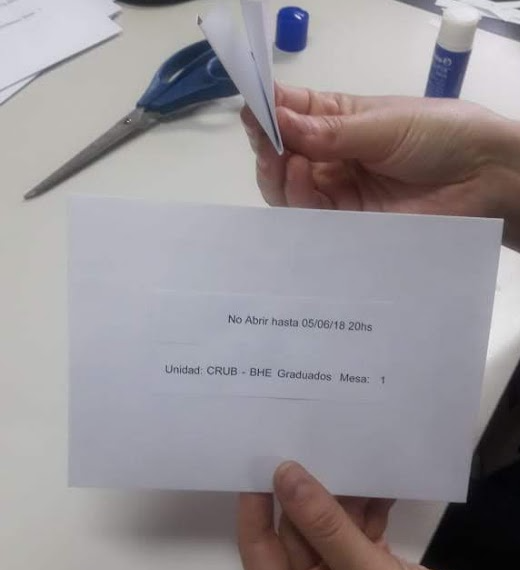
\includegraphics[scale=0.5]{img/jKz6EB2F9Z.png}
    \end{center}
  \caption{Ejemplo Sobre enviado dentro de la urna de la mesa nº1}
  \label{graf:ejemploSobre}
\end{figure}

\item Paso 4: Envío de material. Se envía a cada dependencia el material necesario para poder llevar a cabo los comicios, incluyendo un breve instructivo de carga para la Autoridad de Mesa y el sobre cerrado nombrado en el paso anterior (que sólo debe ser abierto al momento de cargar el acta en el sistema).
\item Paso 5: El Acto Electoral se lleva a cabo en las fechas fijadas por el cronograma electoral y cumpliendo con lo especificado en la Ordenanza Nº 1386/13.
\item Paso 6: Escrutinio Provisorio de la Mesa. 
Una vez que haya finalizado el Acto Electoral, las Autoridades de Mesa realizan el escrutinio provisorio de los votos obtenidos en su mesa, para luego completar por duplicado el acta en papel con la información obtenida del recuento. Ejemplo de un acta cargada en la imagen \ref{graf:ejemploActa}.

\begin{figure}[h!]
    \begin{center}
        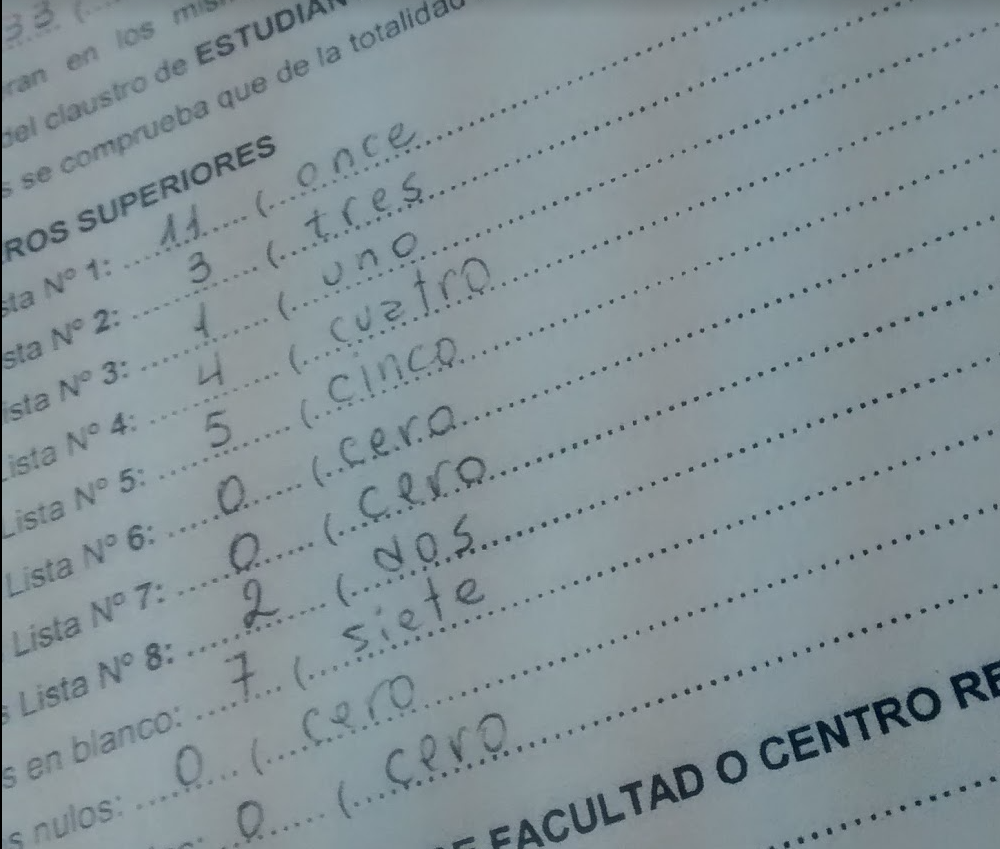
\includegraphics[scale=0.25]{img/f4P4qmrKXY.png}
    \end{center}
  \caption{Ejemplo Acta en papel completada por una Autoridad de Mesa}
  \label{graf:ejemploActa}
\end{figure}

\item Paso 7: Finalizado el Acto Electoral, se habilita el Sistema Gukena para que pueda ingresar cada Autoridad de mesa.
\item Paso 8: Carga y envío de datos en Gukena. Una vez que haya completado el acta papel, la Autoridad de Mesa carga la información de ésta en el Sistema Gukena. Para esto deben ingresar al mismo utilizando el usuario y contraseña contenidos en el sobre. Ejemplo de la pantalla del login en la imagen \ref{graf:ejemploLogin}.
Cuando los datos del acta son confirmados o enviados por la Autoridad de Mesa, estos datos ya no pueden ser editados por este usuario.

\begin{figure}[h!]
    \begin{center}
        
\includegraphics[scale=0.5]{img/ZJ3mtjmmdZ.png}
    \end{center}
  \caption{Pantalla de login para el módulo Autoridad de Mesa y Junta Electoral}
  \label{graf:ejemploLogin}
\end{figure}

\item Paso 10: La Autoridad de Mesa deposita un ejemplar del acta dentro de la urna antes de cerrarla y otro ejemplar es enviado a la Junta Electoral, enviada por los medios disponibles por la Autoridad de Mesa, por ejemplo fax, email, entre otros. 
\item Paso 11: Primera Validación de datos. La Junta Electoral confirma en el sistema que los datos cargados, por las autoridades de mesa, coinciden con las actas papel recibidas, permitiendo corregir cualquier error ocurrido durante el proceso de carga. Para aquellas actas que, por algún inconveniente, no fueran cargadas por la Autoridad de Mesa, como se especifica en el paso anterior, deben ser cargadas por algún miembro de la Junta Electoral.
\item Paso 12: Segunda Validación de los datos. La Secretaria de la Junta Electoral realiza una segunda validación de las actas ya confirmadas por la Junta, en el caso de encontrar diferencias devuelve el acta a la Junta Electoral para su corrección. Si no hay diferencias, entonces dicha acta queda confirmada en el sistema. Una vez que el acta es confirmada ya no puede ser modificada por ningún miembro de la Junta Electoral.

\end{itemize}


\section{Desarrollo}
Gukena ha sido construido por el Grupo de Desarrollo Euclides \cite{euclides} que está integrado por un conjunto de no docentes, estudiantes avanzados y docentes de la Facultad de Informática en la Universidad Nacional del Comahue y funciona bajo la dirección de la Subsecretaría de Tecnologías de la Información de la misma Universidad. El sistema se desarrolló durante los meses de abril a junio a partir del 2015 y los años siguientes, integrándose mejoras evolutivas en cada año.

Para el desarrollo del sistema se utiliza el modelo de ciclo de vida iterativo e incremental, basado en la metodología Scrum, para promover un proceso de construcción ágil y una comunicación fluida con el cliente y, conseguir los beneficios del sistema de forma incremental. En 2015 una primera versión se utilizó para validar las planillas usadas hasta el momento, en 2016 y 2017 se empleó el sistema de forma completa.  En 2018 fue la primera vez que se utilizó en una elección completa considerando los cuatro claustros y la elección de Rector, Decano, Consejeros Directivos y Superiores. Este año se aplicaron mejoras sobre las pantallas accesibles por el público en general que permiten ver los resultados parciales en tiempo real, junto a un histórico de elecciones. Esta mejora fue bien aceptada por la comunidad universitaria permitiendo a los medios de comunicación y público general tener un acceso rápido a los resultados.

En la construcción, diseño e implementación de Gukena se utilizan solamente herramientas de software libre. Se usa el ambiente desarrollo web SIU Toba \cite{toba}, que es desarrollado por el consorcio SIU para soluciones del Sistema Universitario Nacional. Esta herramienta  permite crear sistemas transaccionales en forma rápida, utilizando tecnología web open-source y apunta a agilizar el proceso de construcción y el mantenimiento de los mismos, a través de la reducción de tareas repetitivas, se permite al equipo de desarrollo enfocar su actividad en la lógica del dominio.  El ambiente integra el lenguaje de programación PHP, servidor web Apache, sistema operativo Linux y bases de datos PostgreSQL, entre otros.

Se trabaja utilizando con la filosofía del desarrollo opensource, para contribuir a mejorar el mantenimiento del sistema. Los fuentes son de licencia libre y acceso público, se encuentran disponibles en un repositorio libre
\footnote{Github: \url{https://github.com/svs07uni/gu_kena}} 
con la intención  de que la comunidad de desarrolladores, investigadores, y comunidad de la Universidad puedan acceder al software y analizarlo.
\agregar{reformular descripción MVC toba con fragmentos de código y gráfico}
El ambiente de desarrollo web SIU Toba está basado en el patrón arquitectónico MVC (Model, View, Controller), el cual separa los datos de una aplicación, la interfaz de usuario y la lógica de control en tres componentes distintos. Este patrón permite la separación de conceptos, características que buscan facilitar la tarea de desarrollo de aplicaciones y su posterior mantenimiento. Por lo tanto, este tipo de arquitectura permitió dividir tareas de desarrollo dentro del grupo Euclides y permitió facilitar su evolución por cada año de experiencia. \newline
De manera genérica los componentes de MVC se pueden describir como:
\begin{itemize}
    \item Model (Modelo): Es la representación de la información con la cual el sistema opera y gestiona todos los accesos a dicha información. En este contexto, el Modelo permite guardar y consultar los datos del escrutinio final por cada mesa. Además este componente se encargó de aplicarle las fórmulas necesarias para conseguir el resultado provisorio y/o final de la distribución de escaños. Otra información importante que gestionó fue el log de actualizaciones sobre estos datos, esto permite satisfacer las propiedades de auditabilidad, ya que se registran las actualizaciones por parte de las autoridades de mesa y personal de la Junta Electoral autorizada.
    \item View (Vista): Presenta el Modelo de una manera adecuada para interactuar, es decir, la interfaz de usuario. Se encarga de la representación visual de los datos que gestiona el Modelo. Gukena dispuso una vista por cada módulo de interacción. De manera tal que una autoridad de mesa solo accede a un formulario de carga, una persona autorizada de la Junta Electoral accede a un listado de mesas a validar, y por último una vista más gráfica para el módulo de Resultados. Este componente tiene la responsabilidad de satisfacer las propiedades de usabilidad del sistema.
    \item Controller (Controlador): Responde a eventos e invoca peticiones al Modelo, se encarga de controlar las acciones del usuario y de solicitar los datos al Modelo para comunicarselos a la vista. En Gukena, el Controlador suministró los datos mediante dos vias, una de ellas es la comunicación directa entre Vista y Modelo para los módulos de Autoridad de Mesa y Junta Electoral, sin embargo, para el módulo de Resultados el controlador 'empaquetaba' los datos y los depositaba en archivos JSON, los cuales eran el origen de datos para este módulo.
\end{itemize}
Como se puede ver, una de las ventajas de esta arquitectura MVC es que permite separar los componentes de una aplicación dependiendo de la repsonsabilidad que tienen. Esto respeta el principio de la responsabilidad única.

\section{Testing}
El Testing de un software es cualquier actividad cuyo objetivo es evaluar un atributo o la capacidad de un programa o sistema y determina si logró encontrar los resultados esperados \cite{pan1999software}. Esto no significa que únicamente se utiliza para debuggear un software, el propósito del Testing es asegurar la calidad, verificación y validación, o estimación de confiabilidad. Esta actividad contiene métodos y técnicas destinadas a múltiples propósitos durante las fases dentro de un desarrollo de software. Testing se puede dividir como: testing de correctitud, testing en performance, testing en confiabilidad y testing de seguridad. Un tester puede abocarse a verificar la correctitud de un sistema o software sin conocer internamente su funcionamiento, conocido como testing de caja negra (black-box testing) o por el contrario, planificar los casos de test de acuerdo a los detalles de implementación del software (testing de caja blanca o white-box testing). \newline
Para los casos de test en Gukena participó el equipo que lo desarrollo y usuarios externos a este, como docentes de la Facultad de Informática. Los casos de test involucraron:
\begin{itemize}
    \item Carga de datos erróneos en los formularios de carga del rol Autoridad de mesa, por ejemplo valores negativos en los formularios.
    \item Verificar validaciones integradas en los formularios que conforman la pantalla de carga del rol Autoridad de mesa, por ejemplo las validaciones contra la cantidad de empadronados, validaciones en la cantidad de votantes cargadas en cada formulario.
    \item Verificar cambios de estado de una mesa desde el guardado hasta la validación final por el rol Junta electoral.
    \item Verificar los datos procesados por una cantidad reducida de mesas cargadas contra el resultado final generado por el sistema.
    \item Accesos no autorizados por usuarios no permitidos.
    \item Testing de sobrecarga en consultas paralelas con una cantidad reducida de dispositivos en un mismo instante.
\end{itemize}
\chapter{Elecciones UNComa con Gukena}
\label{Gukena2}
El proceso electoral comienza cuando se definen las fechas de oficialización de padrones y listas, acto electoral, escrutinio provisorio, escrutinio definitivo y proclamación de autoridades electas. Se considera que un sistema de votación exitoso debe cumplir el principal objetivo que es construir la confianza de toda persona involucrada en el proceso. 
Antes del 2015, una única persona era responsable de gestionar correctamente los resultados y distribuir los cargos. La forma de trabajo generaba un cuello de botella en la carga de los datos y una demora de varias horas y hasta días en obtener los resultados finales. \newline
A continuación se detallan los resultados obtenidos luego de comenzar a utilizar Gukena en las elecciones de la universidad agrupados por año. Estas experiencias brindaron un gran aporte a esta tesis al poder analizar la implementación de este sistema en un contexto real.

\section{Experiencia 16 de Junio de 2015}
Para las elecciones celebradas el 16 de Junio de 2015, Gukena se validó con el archivo xls usado en el escrutinio. Este año tuvo información de 18 Unidades Electorales distribuidas en 16 localidades con un total de 34 mesas. 
Ese año, la Universidad renovó integrantes del Consejo Directivo de cada unidad académica y del Consejo Superior de la Universidad, para el claustro de Estudiantes.

De este modo, el sistema se puso a prueba frente a la siguiente información:
\begin{itemize}
    \item La Elección se desarrolló en 18 Unidades Electorales repartidas en 34 Sedes.
    \item 34 mesas distribuidas en las distintas sedes
    \item 9.560 empadronados del claustro Estudiantes
    \item 9 listas para el Consejo Superior
    \item 45 listas para el Consejo Directivo distribuidas entre las diferentes sedes y asentamientos
\end{itemize}
A pesar de que este año no se utilizó el sistema durante el escrutinio, los datos se encuentran disponible en las elecciones históricas presente en la página de Resultados de Gukena.

\section{Experiencia 14 al 17 de Mayo de 2016}
\label{exp2016}
Primera vez que el sistema se integró al proceso electoral de la universidad para las elecciones celebradas desde el 14 al 17 de Mayo de 2016. Gukena contó con información de 18 Unidades Electorales distribuidas en 16 localidades con un total de 77 mesas. 
Ese año, la Universidad renovó integrantes del Consejo Directivo de cada unidad académica y del Consejo Superior de la Universidad, para los claustros de Estudiantes, No Docentes y Graduados. 

De este modo, el sistema operó frente a la siguiente información:
\begin{itemize}
    \item La Elección se desarrolla en 18 Unidades Electorales repartidas en 34 Sedes.
    \item De las 77 mesas distribuidas en las distintas sedes, 18 son para el claustro No docente, 33 son para el claustro Estudiantes y 26 son para el claustro Graduados.
    \item De 22.313 empadronados: 719 son No docentes, 8199 son Estudiantes y 13.395 son Graduados. 
    \item 15 listas para el Consejo Superior, donde 4 son de No docentes, 8 son de Estudiantes y 3 de Graduados.
    \item 121 listas para el Consejo Directivo distribuidas entre las diferentes sedes, asentamientos y distintos claustros.
\end{itemize}

Durante el período de escrutinio, la primer mesa cargada con éxito en el sistema fue la Facultad de Ciencias y Ambientes de la Salud, para el claustro de graduados, 5 minutos después del cierre.\\ 
Con la utilización del sistema, se obtuvo la siguiente información estadística:
66 mesas fueron cargadas directamente por autoridades de mesas siendo el 86\% del total, 39 mesas fueron cargadas entre las 20:00 hs y 21:56 hs, siendo el 51\% del total.\\
11 mesas fueron cargados por la junta electoral, de las cuales una fue corregida en una segunda etapa de verificación.
Sólo 3 valores de actas fueron corregidas por la Junta Electoral, lo que implica un 0,3\% de error en lo cargado por las autoridades de mesa, o lo que es lo mismo un 99,7\% de datos correctos cargados por las autoridades de mesas.

Las razones por las cuales 11 actas no pudieron ser cargadas por las Autoridades de Mesa son las siguientes:
\begin{itemize}
\item La persona destinada a cargar los datos no contaba con experiencia en el uso de la computadora.
\item El extravío del sobre que contenía datos de usuario y contraseña enviado junto a la urna.
\item Problemas con la conexión a Internet.
\end{itemize}

\section{Experiencia 13 al 16 de Mayo de 2017}
Gukena procesó información de 17 Unidades Electorales distribuidas en 14 localidades con un total de 32 mesas. Este año, la Universidad renovó integrantes del Consejo Directivo de cada Unidad Académica y el Consejo Superior en el claustro Estudiantes.

De este modo, el sistema operó frente a la siguiente información:
\begin{itemize}
    \item 32 mesas distribuidas en las distintas sedes
    \item El padrón fue de 9504 estudiantes.
    \item 8 listas para Consejo Superior.
    \item 38 listas para el Consejo Directivo entre las diferentes sedes y asentamientos.
\end{itemize}
  
Del total de mesas se tuvo que 31 mesas fueron cargadas por las autoridades de mesa desde la sede donde se realizó la elección y 1 fue cargada por la Junta Electoral. Todos los datos fueron correctamente cargados, esto quiere decir que ningún dato contenido en las actas debió ser corregido por la Junta Electoral, ni por la Secretaria de la misma.
Durante el período de escrutinio, la primer mesa cargada con éxito en el sistema fue la Facultad de Turismo sede San Martín de los Andes, 3 minutos después del cierre.

De la utilización del sistema, se obtuvo la siguiente información estadística:
31 mesas fueron cargadas directamente por autoridades de mesas, siendo el 97\% del total.

Del total de mesas:
15 mesas fueron cargadas entre las 20:00 hs y 21:20 hs, siendo el 47\%,
%20 mesas fueron cargadas entre las 20:00 hs y 21:40 hs, siendo el 63\%,
%22 mesas fueron cargadas entre las 20:00 hs y 21:50 hs, siendo el 69\% y 
%6 mesas fueron cargadas al día siguiente, siendo el 19\%.
1 mesa fue cargada 	por la Junta Electoral, siendo el 3\% del total.

Ningún acta fue corregida por la Junta Electoral, lo que implica un 0\% de error en la carga realizada por las autoridades de mesa, o lo que es lo mismo un 100\% de datos correctamente cargados por las autoridades de mesas.

\section{Experiencia 2018}
\subsection{Primer vuelta 21 al 22 de Mayo de 2018}
Gukena procesó información de 18 Unidades Electorales distribuidas en 14 localidades con un total de 95 mesas. Este año, la universidad renovó integrantes del Rectorado, Decanato, Consejo Directivo de cada unidad y el Consejo Superior de la UNComa en el claustro Estudiantes, Graduados, No Docentes y Docentes.

De este modo, el sistema operó frente a la siguiente información:
\begin{itemize}
    \item 95 mesas distribuidas en las distintas sedes 
     \item El padrón fue de  30192, distribuidos en 9486 estudiantes, 17481 graduados, 718 no docentes y 2507 docentes.
     \item 5 listas para Rectorado.
     \item 30 listas para Decano
    \item 23 listas para Consejo Superior, distribuidos en 7 del claustro Estudiantes, 5 de Graduado, 5 No Docente, 6 Docente.
    \item 133 listas para el Consejo Directivo: 35 del Claustro Estudiantes, 31 de Graduados, 23 No Docentes, 44 Docentes.
\end{itemize}
Del total de mesas, 94 mesas fueron cargadas por las autoridades de mesa desde la sede donde se realizó la elección y 1 fue cargada por la Junta Electoral, 90 mesas fueron correctamente cargados, esto quiere decir que 5 mesas debieron ser corregidos por la Junta Electoral o por la Secretaria de la misma.

Durante el período de escrutinio, la primer mesa cargada con éxito en el sistema fue la unidad electoral AUZA sede Zapala a las 19:38 hrs. debido a que al ser una mesa con muy poca concurrencia se habilitó la carga minutos antes de las 20:00 hrs.

De la utilización del sistema, se obtuvo la siguiente información estadística:
93 mesas fueron cargadas directamente por autoridades de mesas, siendo el 99\% del total.

Del total de mesas:
45 mesas fueron cargadas antes de las 21:30 hs, siendo el 47\%,
%20 mesas fueron cargadas entre las 20:00 hs y 21:40 hs, siendo el 63\%,
%22 mesas fueron cargadas entre las 20:00 hs y 21:50 hs, siendo el 69\% y 
%6 mesas fueron cargadas al día siguiente, siendo el 19\%.
1 mesa fue cargada 	por la Junta Electoral, siendo el 1\% del total.

5 actas fueron corregidas por la Junta Electoral, lo que implica un 5\% de error en la carga realizada por las autoridades de mesa, o lo que es lo mismo un 95\% de datos correctamente cargados por las autoridades de mesas.

\subsection{Segunda vuelta 4 al 5 de Junio de 2018}
Gukena procesó información de 18 Unidades Electorales distribuidas en 14 localidades con un total de 97 mesas. En esta segunda vuelta, la universidad disputó el Rectorado participando los claustros Estudiantes, Graduados, No Docentes y Docentes.

De este modo, el sistema operó frente a la siguiente información:
\begin{itemize}
    \item 97 mesas distribuidas en 26 de las 34 Sedes de la UNComa.
     \item El padrón fue de  30192, distribuidos en 9486 estudiantes, 17481 graduados, 718 no docentes y 2507 docentes.
     \item 5 listas para Rectorado.
\end{itemize}
Del total de mesas, 96 mesas fueron cargadas por las autoridades de mesa desde la sede donde se realizó la elección y 1 fue cargada por la Junta Electoral y, 97 mesas fueron correctamente cargados, esto quiere decir que ninguna mesa debió ser corregida por la Junta Electoral o por la Secretaria de la misma.

Durante el período de escrutinio, la primer mesa cargada con éxito en el sistema fue la unidad electoral ASMA sede San Martin de los Andes a las 20:02 hrs.

De la utilización del sistema, se obtuvo la siguiente información estadística:
96 mesas fueron cargadas directamente por autoridades de mesas, siendo el 99\% del total.

Del total de mesas:
50 mesas fueron cargadas antes de las 20:40 hs, siendo el 52\%,
%20 mesas fueron cargadas entre las 20:00 hs y 21:40 hs, siendo el 63\%,
%22 mesas fueron cargadas entre las 20:00 hs y 21:50 hs, siendo el 69\% y 
%6 mesas fueron cargadas al día siguiente, siendo el 19\%.
1 mesa fue cargada 	por la Junta Electoral, siendo el 1\% del total.

Ningún acta fue corregida por la Junta Electoral, lo que implica un 0\% de error en la carga realizada por las autoridades de mesa, o lo que es lo mismo un 100\% de datos correctamente cargados por las autoridades de mesas.

\section{Experiencia 14 de Mayo de 2019}
Gukena procesó información de 18 Unidades Electorales distribuidas en 14 localidades con un total de 30 mesas. Este año, la Universidad renovó integrantes del Consejo Directivo de cada Unidad Académica y el Consejo Superior en el claustro Estudiantes.

De este modo, el sistema operó frente a la siguiente información:
\begin{itemize}
    \item 30 mesas distribuidas en las distintas sedes
     \item El padrón fue de  9283 estudiantes.
     \item 27 listas para el Consejo Directivo del Claustro Estudiantes.
     \item 7 listas para Consejo Superior
\end{itemize}
Del total de mesas, 30 mesas fueron cargadas por las autoridades de mesa desde la sede donde se realizó la elección y ninguna mesa fue cargada por la Junta Electoral y, ninguna mesa debió ser corregida por la Junta Electoral o por la Secretaria de la misma.

Durante el período de escrutinio, la primer mesa cargada con éxito en el sistema fue la unidad electoral FAAS sede Puerto Madryn a las 20:01 hrs.

De la utilización del sistema, se obtuvo la siguiente información estadística:
30 mesas fueron cargadas directamente por autoridades de mesas, siendo el 100\% del total.

Del total de mesas:
15 mesas fueron cargadas antes de las 21:10 hs, siendo el 50\%,
%20 mesas fueron cargadas entre las 20:00 hs y 21:40 hs, siendo el 63\%,
%22 mesas fueron cargadas entre las 20:00 hs y 21:50 hs, siendo el 69\% y 
%6 mesas fueron cargadas al día siguiente, siendo el 19\%.

Ningún acta fue corregida por la Junta Electoral, lo que implica un 0\% de error en la carga realizada por las autoridades de mesa, o lo que es lo mismo un 100\% de datos correctamente cargados por las autoridades de mesas.

\section{Velocidad de carga}
Como se puede ver en la Tabla \ref{tab:comparativaExperiencias} entre las 21:00 y 22:00 hrs se logró un 50\% de carga del escrutinio  en cada elección. Se puede observar que las elecciones en el año 2018 fue el más abarcativo participando la totalidad de la universidad y con renovación de todos los cargos, sin embargo esto no afectó a la velocidad de carga ya que solo generó que 30 min. más tarde comparado al año anterior se llegó a conseguir el 50\% de la totalidad de los datos. Como Gukena obliga a realizar el escrutinio de la mesa de forma manual no se podría reducir este tiempo de espera sin poner en riesgo la eficacia del proceso electoral. Otra característica que se pudo observar fue la velocidad de aprendizaje de las personas involucradas. Como se puede ver en el 2016, primer año en que Gukena comenzó a utilizarse en este ámbito se logró una buena velocidad de carga no variando en los años siguientes, teniendo en cuenta el tamaño de cada elección.

\begin{center}
\begin{table}[h]
  \begin{tabular}{|l|l|l|l|l|l|}
    \toprule
Año & Cant.  & Cant. & 50\%& Cargos & Claustros\\
&Mesas & Empadronados&carga&&\\
    \midrule
    2015 & 34 & 9.560 & - & \tabitem Consejo Superior & \tabitem Estudiantes \\
    & & & & \tabitem Consejo Directivo & \\
    \hline
    2016 & 77 & 22.313 & 21:56 & \tabitem Consejo Superior & \tabitem Estudiantes \\
    & & & & \tabitem Consejo Directivo & \tabitem No docentes \\
    & & & & & \tabitem Graduados \\
    \hline
    2017 & 32 & 9.504 & 21:10 & \tabitem Consejo Superior & \tabitem Estudiantes \\
    & & & & \tabitem Consejo Directivo &  \\
    \hline
    2018 (1ª) & 95 & 30.192 & 21:50 & \tabitem Consejo Superior & \tabitem Estudiantes \\
    & & & & \tabitem Consejo Directivo & \tabitem No docentes \\
    & & & & \tabitem Rector & \tabitem Graduados \\
    & & & & \tabitem Decano & \tabitem Docentes \\
    \hline
    2018 (2ª) & 97 & 30.192 & 20:30 & \tabitem Rector & \tabitem Estudiantes \\
    & & & & & \tabitem No docentes \\
    & & & & & \tabitem Graduados \\
    & & & & & \tabitem Docentes \\
    \hline
    2019 & 30 & 9.283 & 21:00 & \tabitem Consejo Superior & \tabitem Estudiantes \\
    & & & & \tabitem Consejo Directivo &  \\
    \bottomrule
  \end{tabular}
  \caption{Comparativa Experiencias UnComa}
\label{tab:comparativaExperiencias}
\end{table}
\end{center}

%\agregar{pk: agregar gráfico de experiencias y conclusión - HECHO}

\begin{figure}[h!]
    \begin{center}
        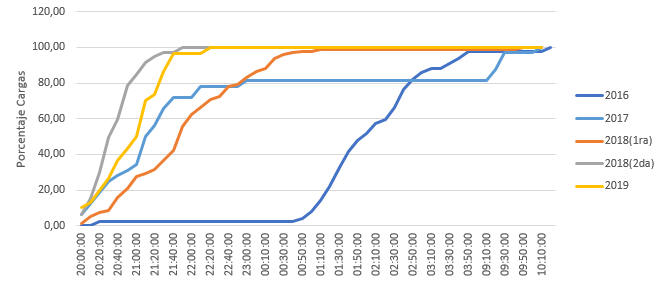
\includegraphics[width=\textwidth]{img/experienciasPorcCarga.png}
    \end{center}
  \caption{Porcentaje de carga}
  \label{graf:experienciaPorcCarga}
\end{figure}

A partir de estas experiencias podemos ver en la Figura \ref{graf:experienciaPorcCarga} el porcentaje acumulado durante el periodo de escrutinio para cada acto electoral.  \newline
En el año 2016, primer año que se utilizaba Gukena, se logró una buena velocidad de carga computando el 60\% de las mesas a las 22:30 hrs. Todo sistema nuevo requiere su periodo de aprendizaje y adaptación sobre los usuarios. Se puede comentar que en este año se cargaron algunas actas directamente por la Junta Electoral o la Secretaria cuando se recibían las urnas por distintas razones listadas en la subsección \ref{exp2016}. \newline
Analizando el tamaño del dominio, Gukena logró cubrir con éxito el proceso electoral en el 2018 cuando se requerían elegir todos los cargos de la UNComa y todos los claustros debían votar. Como se puede observar en el año 2018 (1ra vuelta) se logró una muy buena velocidad de carga logrando el 60\% del escrutinio luego de 2 horas de terminado el acto electoral.\newline
En la Figura \ref{graf:experienciaPorcCarga} se observa que el momento de mayor carga de cada año fluctúa entre las 20.30 y 23.00 hrs., notándose que por cada año nuevo que se utilizó Gukena se fue reduciendo el tiempo de espera para lograr la mayoría de las mesas cargadas. El sistema no modificó su integración dentro del proceso electoral por lo tanto, esta velocidad se logró por el aprendizaje de los usuarios. Sin necesidad de involucrar al sistema en la primer etapa del proceso, en la emisión del voto.

En la Figura \ref{graf:provincialConGukena} se muestra el porcentaje de carga de Gukena y las elecciones provinciales en Río Negro, Córdoba, Neuquén analizadas en la subsección \ref{analisisComparativoProvincial}.
Debido a que el horario del cierre del escrutinio a nivel provincial y en UNComa son distintos se debió modificar los tiempos de cargas de Gukena restándole 2 horas para que sean comparable entre ellas. Otra diferencia entre estas elecciones son la cantidad de mesas escrutadas, siendo mucho menor en UNComa, por lo tanto, se tomaron las experiencias de Gukena con mayor cantidad de mesas las cuales fueron las elecciones del 2018 (1ra y 2da vuelta). 


\begin{figure}[h!]
    \begin{center}
        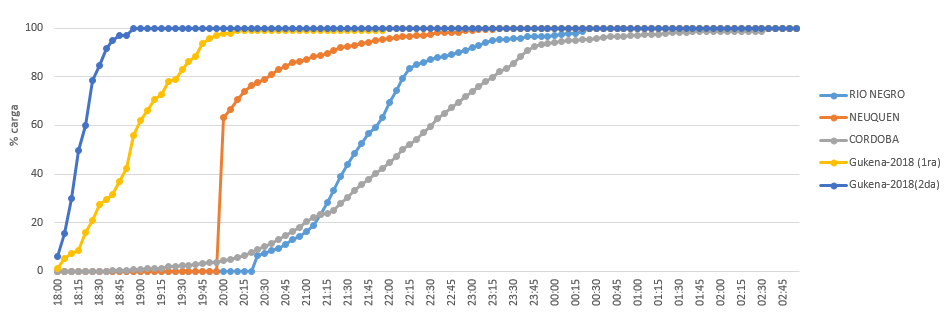
\includegraphics[width=\textwidth]{img/provincialGukena.png}
    \end{center}
  \caption{Porcentaje de carga comparativo}
  \label{graf:provincialConGukena}
\end{figure}

En la Figura \ref{graf:provincialConGukena} muestra distintos procesos electorales que involucran tecnología en diferentes etapas. En Rio Negro se involucró tecnología en la transmisión de resultados desde nodos zonales, manteniendo boletas partidarias en papel y escrutinio manual. Como variante a las elecciones de Río Negro, Córdoba sólo se diferencia en que utiliza la boleta única papel. Para ambas elecciones se puede ver que logra una curva constante y un crecimiento lento durante toda la noche de escrutinio. Por otro lado, las elecciones de Neuquén que utilizan tecnología en todo el proceso electoral muestran un pico de crecimiento a las 20:00 hrs. Finalmente, Gukena que utiliza tecnología en las etapas siguientes al escrutinio manual también consigue una buena velocidad de cómputos. Ambos logran en poco tiempo conseguir la mayoría de las mesas escrutadas disponibles en el sistema. Para esto ambos sistemas tuvieron que pasar por un aprendizaje por parte de los usuarios. En Gukena la cantidad de personas involucradas es menor que en el sistema BUE, ya que este último involucró capacitación tanto de los técnicos (mínimo uno por escuela), autoridades de mesa y de cada votante. Gukena sólo necesita la capacitación de una persona por mesa (Autoridad de Mesa), a quien se le envió un instructivo en papel incluido en el kit de la urna. Esta ventaja de Gukena reduce notablemente el presupuesto en capacitación con respecto al sistema BUE.

La encuesta de la opinión pública del sistema BUE, descrita en la subsección \ref{encuesta} nos dio evidencia de que los electores no tenían conocimiento del chip integrado en la boleta única electrónica y desconocían la existencia de la validación de estos chips usando la máquina. 
Además se pudo observar que las autoridades de mesa en muchos casos, dejan a las máquinas la responsabilidad del conteo usando el chip y no realizan un escrutinio manual para su validación.
Por lo tanto, se puede concluir que la curva del escrutinio en Neuquén es buena pero sin seguridad de que las máquinas realizaron un conteo correcto o que el chip integrado almacenó el dato correcto del votante. Gukena al no involucrarse en las etapas de emisión del voto y en el escrutinio de la mesa, logró una buena curva del escrutinio como en Neuquén, sin poner en riesgo la integridad del voto. 

\input{cap4}
\chapter{Conclusiones}
\label{conclusiones}
%\cambiar{El gráfico comparativo que hace con Gukena y los otros sistemas electorales no va en las conclusiones. - HECHO: Se quitan los gráficos}
%\cambiar{Para el caso de colocar esta descripción antes, aclara que las mesas cierran en distintos horarios, pero puede ponerlas todas al mismo horario de cierre X, y en vez de nombrar las horas finales de carga de mesas, poner directamente “luego de 90 minutos estaban el 90\% de las mesas cargadas” por ejemplo.}
%\cambiar{Repite párrafos completos, ¿otra vez la figura 6.2 y figura 6.3? - HECHO: se quitan los gráficos}

El proceso electoral se divide en 5 etapas según el modelo de referencia \cite{conicet} (Figura \ref{graf:modeloReferencia})
\begin{figure}[h!]
    \begin{center}
        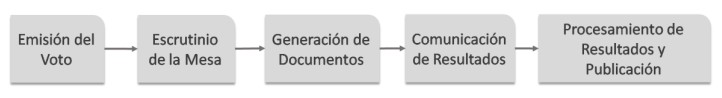
\includegraphics[width=\textwidth]{img/modeloReferencia.png}
    \end{center}
  \caption{Modelo de Referencia}
  \label{graf:modeloReferencia}
\end{figure}
\newline

Incluir tecnología sobre alguna de estas etapas consigue mejoras sobre el sistema electoral, por ejemplo acelerar la velocidad de procesamiento. Sin embargo, puede incluir problemas como  poner en riesgo la integridad y secreto del voto, principalmente cuando se incluye en la primera fase, Emisión del voto. En esta tesis se analizaron experiencias a nivel nacional e internacional, en muchos casos, luego de varios intentos los responsables de estas elecciones resolvieron no continuar con un sistema de voto electrónico. Un ejemplo de ello es Holanda, que luego de 9 años utilizando un sistema electrónico se demostraron las vulnerabilidades del sistema y el gobierno decidió volver al proceso electoral tradicional en papel. Un sistema electoral exitoso debe garantizar la confianza de toda persona involucrada, para ello, es necesario entender todo el proceso interno del sistema. Sin embargo, sólo un grupo reducido de personas relacionadas al área de sistemas computacionales comprenderán el funcionamiento de este proceso, aún así, no existe un método formal de validación que avale un sistema electrónico correcto. 

Luego de analizar en esta tesis las ventajas y desventajas de implementar tecnología en cada una de las etapas del proceso electoral, se expone el desarrollo e implementación del sistema Gukena. Este sistema mantiene las primeras 3 etapas (Emisión del voto, Escrutinio de la Mesa y Generación de Documentos) de forma tradicional en papel y manual. Gukena se integra en las etapas de Comunicación de Resultados, Procesamiento de Resultados y Publicación. La etapa de Comunicación de resultados es de manera descentralizada mediante un ``acta electrónica'' cargado por cada autoridad de mesa al finalizar el escrutinio. El sistema se encarga de procesar y publicar los resultados en tiempo real a medida que se van cargando los datos en este acta.

Gukena se incluye en las elecciones de la UNComa y consigue un cambio notable en este proceso, tanto a nivel de velocidad del escrutinio como de claridad y transparencia en los resultados finales. Previo a utilizar Gukena, estas elecciones eran administradas por una única persona. Todo este proceso abarcaba varios días debido a que se generaba un cuello de botella. Gukena logra distribuir la carga de trabajo a un grupo de personas, las autoridades de mesa y la Junta Electoral.

Por lo tanto, el proceso electoral de la UNComa con Gukena queda de la siguiente manera:
\begin{enumerate}
    \item Emisión del Voto: Tradicional en papel, colocando el sufragio en el sobre.
    \item Escrutinio de la Mesa: Tradicional escrutinio manual.
    \item Generación de Documentos: Tradicional utilizando el acta en papel.
    \item Comunicación de Resultados: Formulario de Gukena donde cada autoridad de mesa vuelca los datos del acta en papel.
    \item Procesamiento de Resultados y Publicación: Gukena realiza el procesamiento aplicando las fórmulas de ponderación y publica los resultados provisorios en tiempo real en su página web pública. Los datos recibidos de cada acta se validan por la Junta Electoral a través del sistema.
\end{enumerate}

En este documento se analizaron las experiencias de Gukena dentro del ámbito de la UNComa y se pudo observar que con una mínima incorporación de tecnología en el proceso electoral, sin invadir la etapa de Emisión del Voto, se lograron buenos resultados de velocidad del escrutinio sin afectar el secreto del voto y la auditabilidad del sistema.

Una de las ventajas adicionales que introdujo Gukena a la transparencia del proceso es la visualización de información histórica de elecciones a partir del 2015, información que no era pública y de fácil acceso previamente. Otra ventaja agregada es facilitar la comprensión de la fórmula del voto ponderado, explicada en conjunto con los resultados de cada elección, accesibles en cualquier momento desde cualquier dispositivo con acceso a Internet a través de la página web. Gukena fue expuesto en el artículo presentado en la JAIIO describiendo lo planteado en este capítulo \cite{articuloGukena}.

Además, en este trabajo se agregó la evaluación del escrutinio de las elecciones en la provincia de Córdoba, Rio Negro y Neuquén realizadas en el año 2019, junto con las experiencias de Gukena en el año 2018. Cada una de estas elecciones aplicó distintas técnicas de conteo durante el proceso electoral, la velocidad de las elecciones en Córdoba y Río Negro es constante durante todo el escrutinio. Por otro lado, en la provincia de Neuquén y con Gukena se logró en poco tiempo conseguir la mayoría de las mesas escrutadas disponibles en el sistema, satisface el objetivo de reducir los tiempos con respecto al sistema tradicional. Sin embargo, el horario de finalización del escrutinio no varía mucho en cada elección, por lo tanto, aplicar tecnología en cualquier etapa del proceso electoral no genera un impacto notable en el horario de publicación de resultados.

Otra característica, en las elecciones de Neuquén se deben capacitar los técnicos (mínimo uno por escuela), las autoridades de mesa y cada votante. En cambio, Gukena sólo necesita la capacitación de una persona por mesa, cada autoridad de mesa recibe un instructivo en papel incluido en el kit de la urna. Esta ventaja de Gukena reduce notablemente el presupuesto en capacitación.

Además del desarrollo e implementación de Gukena, como aporte a esta tesis, se presenta una encuesta realizada a los votantes de Neuquén Capital con respecto al sistema BUE. Más de la mitad de los encuestados no conocía la existencia del lector de chip, por lo tanto, se podría concluir que si existieron errores de escritura no fueron detectados. A partir de este análisis se sugirió a nivel provincial un cambio de protocolo en las elecciones electrónicas en la Junta Electoral Provincial. Este cambio consta de una validación de manera aleatoria de las máquinas BUE durante el acto electoral, agregando una verificación más dentro de este proceso. La validación consta de imprimir una boleta y verificarlo con el lector de la máquina corroborando su correcta escritura del chip. Esta sugerencia fue tomada en cuenta y es aplicada a partir del 2019 en las elecciones dentro de la provincia del Neuquén.


\section{Trabajos Futuros}

Como trabajo sugerido a futuro en Gukena está asociado a la posibilidad de incluir la Boleta Única en papel dentro del sistema electoral de la UNComa. Esta boleta consiste en un solo papel por categoría a votar, por ejemplo para las elecciones en UNComa del año 2018, descripto en la Sección \ref{gukena2018}, cada votante va a disponer de 4 boletas únicas en papel, uno por cada categoría. Esto reduce notablemente la gran cantidad de papeles y en presupuesto general, actualmente se dispone de un papel por cada lista y por cada categoría. Las ventajas de la Boleta Única en Papel y un ejemplo de ésta se describe en el Anexo \ref{BU}. El posible cambio a nivel de proceso electoral impacta en el formulario de carga de Gukena, obligando a incorporar nuevas validaciones o cambios, como por ejemplo, la cantidad de votantes puede diferir por categoría, validación no contemplada actualmente. Esto aplica a la propiedad de calidad, descripta en la sección \ref{propiedadesCalidad}, de cumplir con las normativas vigentes del proceso electoral, Gukena debe adaptarse a cualquier cambio sobre el proceso electoral en UNComa. 
%\cambiar{¿Por qué se coloca un anexo de la boleta única en papel? y Gukena?}

Un cambio pendiente en Gukena a nivel desarrollo, es incluir las actas escaneadas o imagen dentro del formulario de carga, para que estén disponibles en la página web. Actualmente, los usuarios (Autoridades de Mesa más lejanos del centro de cómputos) deben enviar la imagen del acta por algún medio que logre llegar a la Junta Electoral para su validación. Como no existe una única vía de comunicación, se debe estar atento en reconocer el medio utilizado por cada autoridad de mesa: fax, mensaje privado, email o presencial. Con una carga de archivos de imágenes dentro de los datos en el formulario de carga, se generaría un único medio de fácil acceso por la Junta Electoral y la Secretaria para su validación.
Agregar este cambio no reemplazaría el envío al centro de cómputos del acta en papel y la urna con los votos, como registro físico auditable de la elección. 

\label{Anexos}
\appendix
\clearpage
\addappheadtotoc
\appendixpage
\chapter[Anexo I: Fisc. Virtual/Inf. para elecciones en Neuquén]{Anexo I: Fiscalización Virtual/Informático para elecciones en Neuquén}
En Febrero de 2019 se participó como fiscales informáticos para Unidad Ciudadana en las elecciones provinciales de Neuquén para ese mismo año. La misión de un fiscal es verificar y auditar el sistema a utilizar en la emisión de sufragio, las boletas y el sistema de recuento provisorio. El objeto es detectar cualquier situación que pudiera poner en riesgo la transparencia o la equidad en los comicios, o llevar a confusión al elector. Para llevar adelante este proceso la Justicia Electoral de Neuquén convocó a diferentes agrupaciones políticas para auditar la quema de DVDs y la prueba de transmisión. Estos DVDs son el medio para iniciar y habilitar las máquinas para su posterior uso en la votación. La prueba de transmisión se ejecuta sobre una máquina que contiene los mismos componentes que las máquinas de votación pero utiliza otro software, esta máquina además se conecta a internet y ejecuta un sistema preparado para transmitir los datos de escrutinio. 

\section{Quema de DVDs el día 28/02/2019}
Se participó durante la audiencia para la quema de 2000 DVDs (1504 mesas + 500 de backup) utilizados para iniciar las máquinas del sistema de boleta única electrónica (BUE). \newline
Esta actividad se realizó en una sala dividida en dos secciones, una fue utilizada para los fiscales de diferentes partidos, y otra para personas de la justicia y la empresa.  \newline
El evento comienza con una explicación del proceso a realizar por parte de la Justicia Electoral.  La organización informa que existe un solo software utilizado para toda la elección. Cada autoridad de mesa contará con una tarjeta personal con un chip que permite activar las categorías disponibles para la mesa que corresponda. Es decir, en las localidades donde sólo se elige gobernador, el sistema muestra Gobernador-Diputados-Consejeros y en las ciudades donde también se elige intendente, se muestra además los Intendentes y Concejales de esa localidad. \newline
Luego se muestra un DVD (el master) cuyo contenido no es accesible, del cual solo se conoce que se utiliza el método de hash sha512sum da la firma: \newline
8d7b20cf8f3d101a3253ca7af1ae91c0d24cd36af3371ad65daa295f224f83a7e89d0ccbe21fabb2393c1b \newline 153118c369423b92de5a5a1204f0c84e5c7f2687d7  \newline
Se procede con la primera copia de 6 DVDs y se valida que coincida la firma con el DVD master.  
Se pone a disposición 3 máquinas (una de las cuales no inició y fue reemplazada) para probar el sistema. Se visualiza el sistema desde un punto de vista funcional, haciendo todo el proceso desde la apertura de la mesa hasta el cierre. En las pruebas hechas no hubo errores detectados. Se testearon tres disposiciones de candidatos (Neuquen Capital, Centenario y Chos Malal) por un periodo de 15 minutos. 
Al momento de responder consultas sobre el desarrollo del sistema, los referentes presentes en la exposición responden que no poseen conocimientos técnicos sobre el software utilizado. Además, se consulta sobre el sistema que se encarga de transferir los datos desde la escuela al centro de cómputos, respondiendo que la máquina utilizada para tal fin es la misma con la cual se realizan los votos, con la diferencia que el DVD utilizado es distinto y esta máquina se encuentra apartada de las demás conectada a la red de internet de la escuela. \newline
En resumen, este día se auditaron las copias que se realizaron verificando que posea el mismo hash que el master.  Del master se pudieron hacer algunas pruebas de funcionamiento correcta, pero no se permitió auditar el código fuente. Por lo tanto, no se pudo garantizar: 
 \begin{itemize}
     \item que la disposición de las opciones sea siempre aleatoria y que se presenten todos los candidatos 
     \item que imprima en la boleta lo seleccionado 
     \item que el contenido del chip sea igual a lo impreso en la boleta papel 
     \item que el proceso de conteo sea correcto 
     \item que se imprima el resultado final correcto 
     \item que el contenido del chip del acta de cierre sea igual a lo impreso en el acta papel 
     \item que los datos que se transfieren de la escuela sean iguales al acta papel
     \item la integridad de los datos
     \item el secreto del voto
 \end{itemize}


\section{Prueba de transmisión el día 07/03/2019}
Se participó durante la prueba de conectividad y transmisión de datos desde la Escuela CEPEN 46, y la recepción de datos en el Centro de Cómputos Ubicado en la Ciudad Judicial.\newline
Durante las pruebas en la escuela participaron, personal de la Justicia Electoral, personal no informático de la empresa que provee el servicio, los técnicos que van a encargarse de realizar la tarea el siguiente domingo 10/3/2019 y fiscales informáticos de varias listas.\newline
La simulación del proceso de trasmisión de los datos de cada mesa se realizó en una máquina igual a la que se utilizan para votar, pero inicia con otro DVD y con conexión, a través de un cable Ethernet, a la red de la escuela. Primero se realiza la prueba de conectividad con validación del canal, con un certificado digital que se encuentra en un DVD, a su vez encriptado con una clave que llega por mensaje de texto a los técnicos, en una aplicación móvil que utilizan para realizar el seguimiento de la escuela.\newline
Asegurada la conexión, se acercó el chip de un acta con el resultado de una mesa de prueba, se validó que en ese caso la máquina mostrara lo mismo que lo escrito en la boleta y se transmitió de forma correcta. Este proceso se repite con otras dos actas. Luego se apaga la máquina, se la lleva a otro lugar y se repite el proceso transmitiendo un acta, pero esta vez a través de la conectividad brindada por un modem 4G.
Nos fue informado que en primera instancia se utilizará la red de la escuela, si no funciona se utilizará un modem 4G y en última instancia antenas de Internet satelital.\newline

Posteriormente, durante el evento en la Ciudad Judicial se sumaron a la comitiva dos informáticos de la empresa, los cuales muestran una tablet conectada vía WiFi a la notebook del desarrollador, esto muestra la llegada de los datos de las mesas que han sido enviadas desde la escuela. Nos fue informado que hay dos formas de visualización de datos: una API (Application Programming Interface) en formato json y un archivo en formato CSV que da los datos por mesa. Además, comunican que el procesamiento de las actas con boleta en papel se envían escaneadas mediante el protocolo FTP a un centro de cómputos que la empresa tiene en Buenos Aires, donde se realizaría la carga en el mismo sistema que recibe los datos de las mesas con el sistema electrónico.\newline
El personal describió el Workflow desde que llega un acta al centro de cómputos hasta que se publica: cada acta pasa por un proceso de validación automático con dos conjuntos de reglas, de las cuáles sólo describieron que no haya más votos que los empadronados y que los votos en blanco no sean "demasiados", sin mayores precisiones. Si el acta no cumple con una de las reglas pasaría a un proceso de validación manual a ser realizado por referentes de la Justicia. En caso de pasar los dos controles automáticos o ser aprobada manualmente por los referentes de la Justicia pasaría a publicación.\newline

Comentaron que los resultados llegarían al sitio oficial público a las 19hs o cuando se alcance el 20\% de las mesas cargadas, con acceso previo únicamente por la Justicia. Además, fiscales informáticos que se encuentren en el centro de cómputos van a poder acceder a un sistema que visualiza el Workflow de todas las actas.\newline

Como resumen de la actividad realizada y considerando que no se ha realizado ningún tipo de auditoría a los sistemas, no se puede garantizar:

\begin{itemize}
    \item el funcionamiento correcto en un escenario real, ya que las pruebas fueron realizadas en un contexto controlado y asilado y esto no implica ningún tipo de garantías.
    \item la seguridad del canal de comunicación, este día sólo se informó el método de comunicación pero no se permitió auditar este canal y no se contó con documentación técnica detallada.
    \item el sistema de validación, no son públicas las reglas automáticas de validación ni el criterio a seguir en el caso manual.
    \item el sistema de publicación de los resultados, a pocos días de la elección el sistema aún se encontraba en desarrollo, por lo tanto no se pudo auditar.
    \item el sistema de envío de las imágenes de las actas de boleta papel, podemos decir que el protocolo utilizado (FTP) no es seguro.
\end{itemize}
El 8/03/2019 se envía el documento señalando que la API de resultados se encuentra publicada en https://neuquen.votar.com.ar/API\_Resultados\_Neuquen\_2019.zip, junto con una serie de direcciones web donde se encontraría publicada la información. Se transcribe una a modo de ejemplo: http://datosoficiales.com/resultados/NE/1/86/1276/DIP.json. 

\section{Catalogar actas el día 10/03/2019}
Los resultados, como se nombró anteriormente, se publicaron en: \newline https://www.datosoficiales.com/#resultados/GOB/NE 
\newline Se utilizó un sistema para catalogar actas escaneadas en neuquen.cba3.com.ar \newline
Se participó en la carga de actas físicas que fueron digitalizadas al sistema de Unidad Ciudadana. Se observaron actas tanto generadas por una máquina de boleta única electrónica como actas elaboradas manualmente, ya que en la gran mayoría de la provincia se utilizó el método de Boleta Única Electrónica (BUE), un total 1397 mesas; y las localidades más pequeñas no lo utilizaron, siendo 110 mesas \cite{eleccionesNeuquenBUE} \newline
A partir de las 18:30 hrs. aproximadamente se ingresó a la página como catalogador y se tuvo acceso a tres acciones principales: 

\begin{itemize}
    \item \underline{Clasificar actas: }A partir de una imagen se rellena un formulario indicando la mesa que correspondía tal acta observada.
    \item \underline{Cargar resultados: }A partir de una imagen del acta se ingresan los valores de cada partido rellenando un formulario. Debido a la acción anterior, este formulario ya se encontraba relacionado a la misma mesa que figuraba al acta en la imagen.
    \item \underline{Chequear una mesa: }En base a un formulario ya rellenado con valores de cada partido y su totalizador, se verifica contra la/s imagen/es tales valores. En caso de no corresponder se informa el error. Sin posibilidad de editar el error en el caso que el formulario posea valores incorrectos.
\end{itemize}
Cerca de las 21 hr. se finalizó este proceso. Como propia experiencia, sólo observé algunas actas que no correspondían al formulario a validar, estos pocos casos fueron reportados. 
Al solo observar imagenes de actas ya impresas, no se puede garantizar:
\begin{itemize}
    \item el funcionamiento correcto de la máquina que realizó el escrutinio de la mesa y generó este certificado.
    \item que los datos impresos que se visualizaron esté correctamente impreso en el chip que se escanea para transmitir los datos.
    \item que la transmisión de los datos sea correcta, es decir, los datos impresos  en el acta se haya recibido correctamente en el centro de cómputos del sistema.
\end{itemize}

\section{Resultados}
Neuquén ya pasó por varias jornadas electorales utilizando este sistema de boleta electrónica BUE, tanto en municipios como la elección a nivel provincial. Particularmente las elecciones a gobernador del día 22/09/2019 generó polémicas cuando el gobernador Omar Gutierrez notó que al verificar su boleta, esta no reflejaba su intención. Esto culminó con una nueva boleta para generar el voto con éxito, justificándose que seguramente el chip estaba dañado \cite{errorOmarGutierrez}.  Por otro lado, se generaron denuncias por irregularidades en algunas máquinas, algunos votantes notaron que al votar se imprimía otra elección. Como detalló la fiscal general de UC-Frente Neuquino, en la escuela 56 de Neuquén Capital se intervino la máquina ``porque la gente apretaba una cosa e imprimía otra''. Registró 5 casos en la misma máquina en la cual las boletas tuvieron que ser anuladas \cite{errorNeuquen}. \newline
Para las elecciones municipales del día 10/03/2019, como se detalló anteriormente, la Junta Electoral facilitó una API como medio de interacción con los datos de esta elección. 


\chapter{Anexo II: Documentación Base de Datos Gukena}
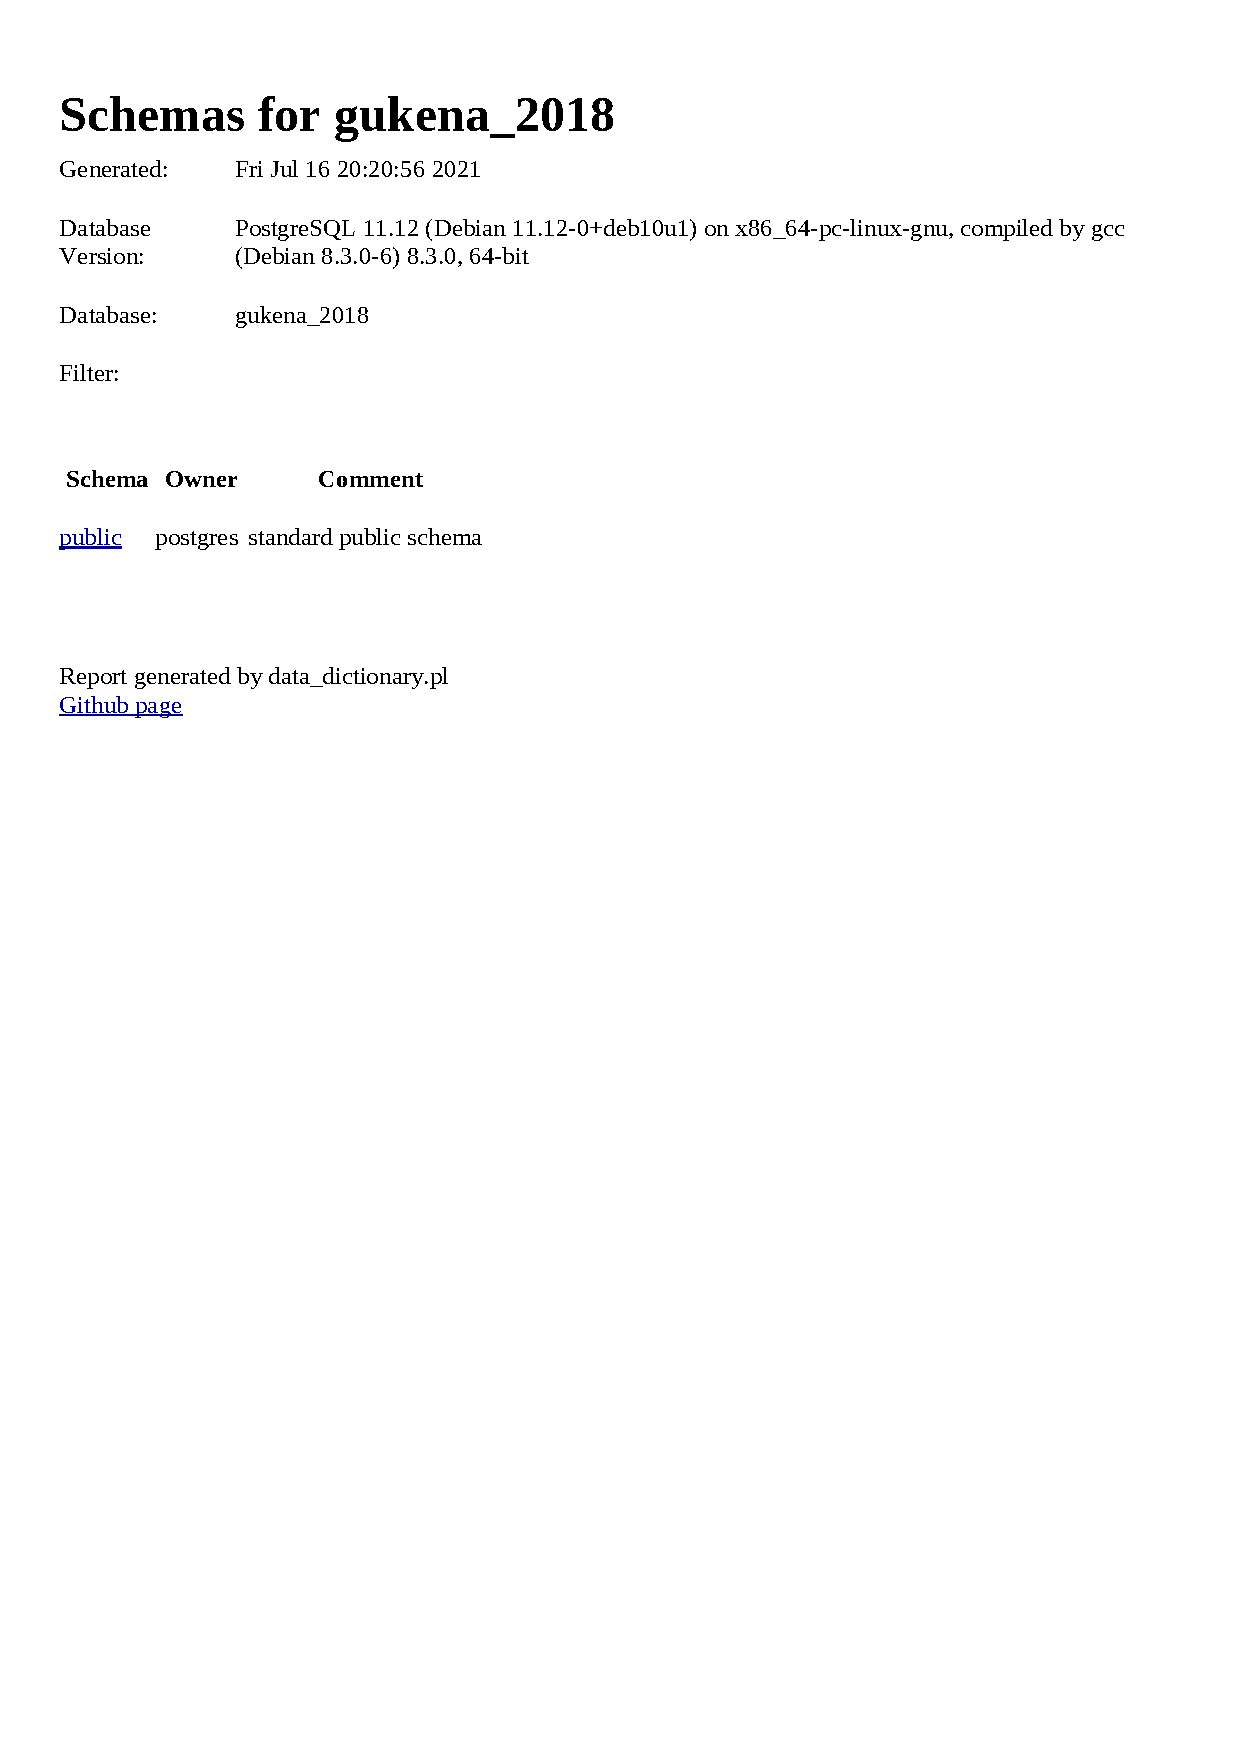
\includepdf[pages=-]{pdf/squema.pdf}
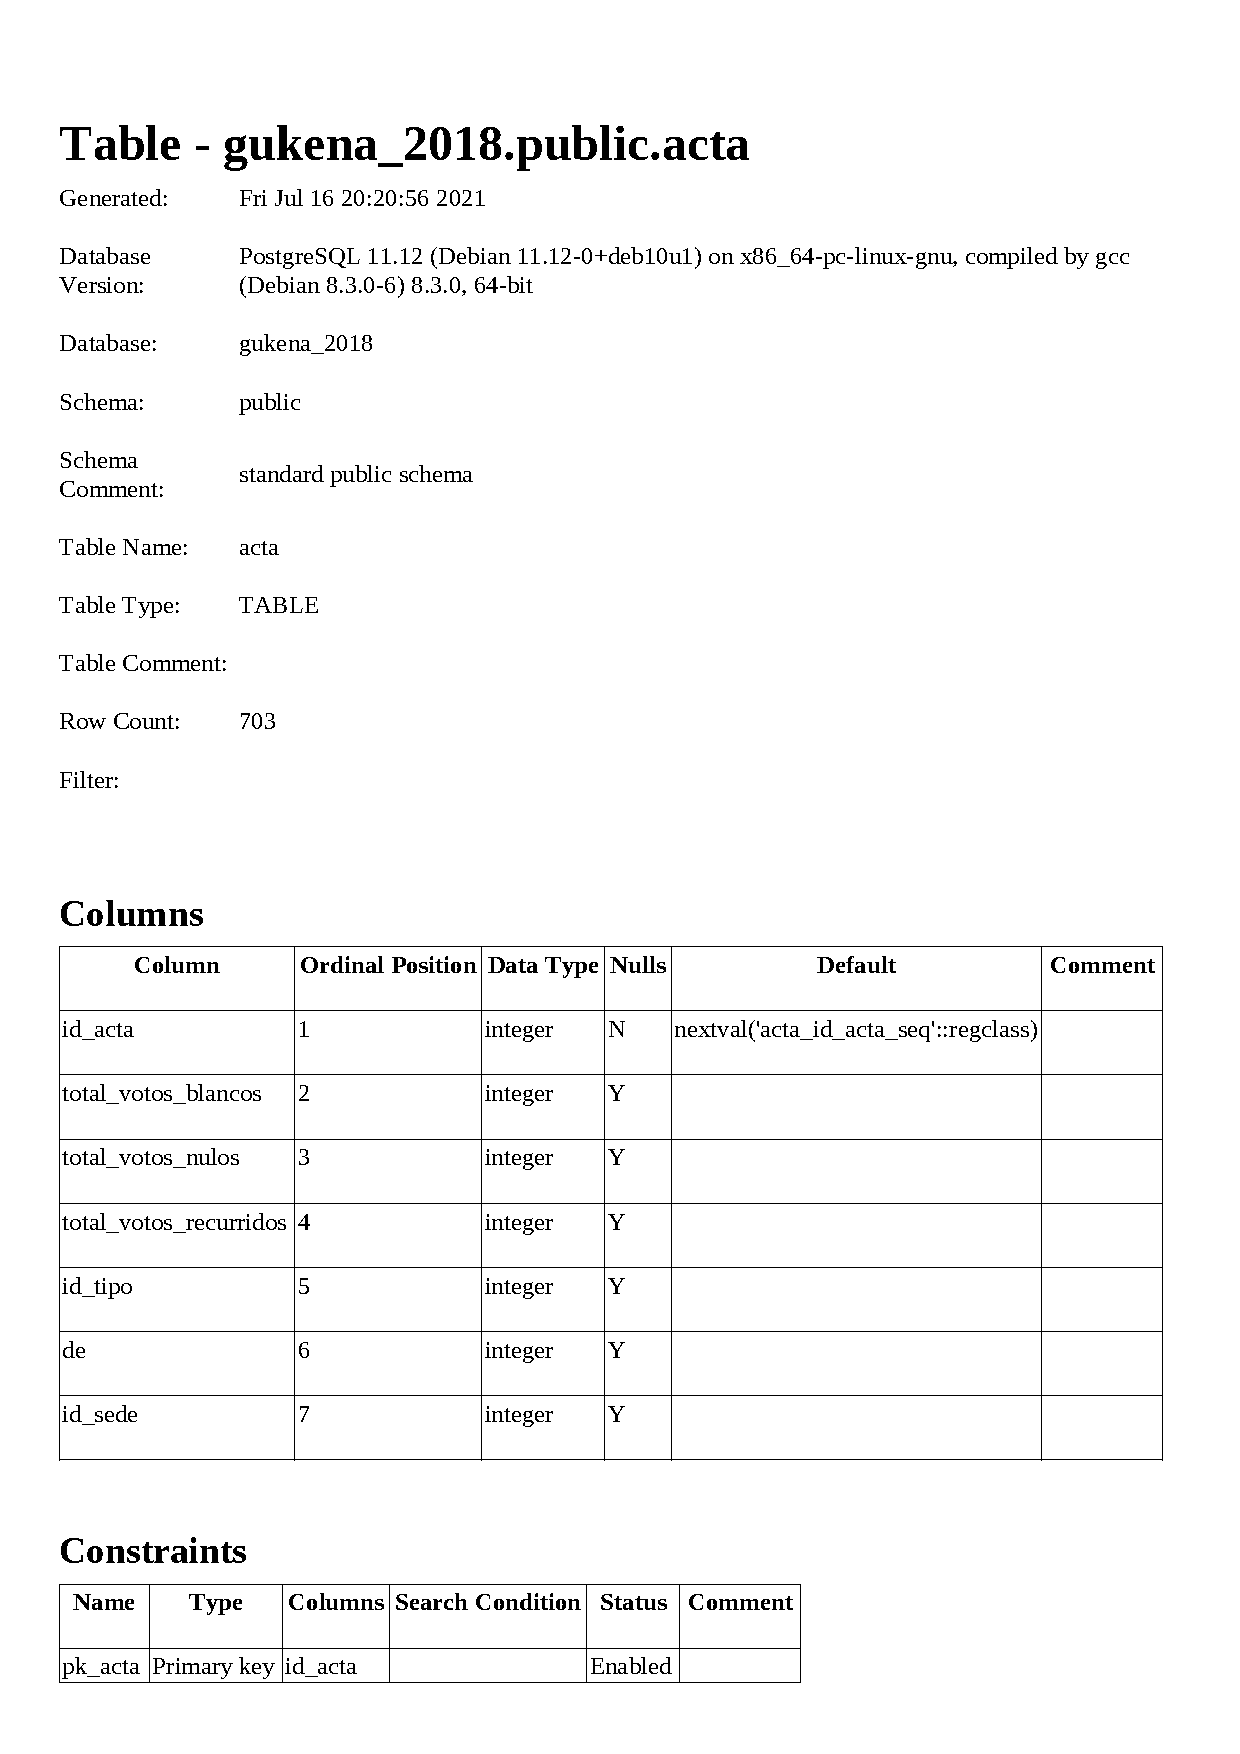
\includepdf[pages=-]{pdf/tables.pdf}
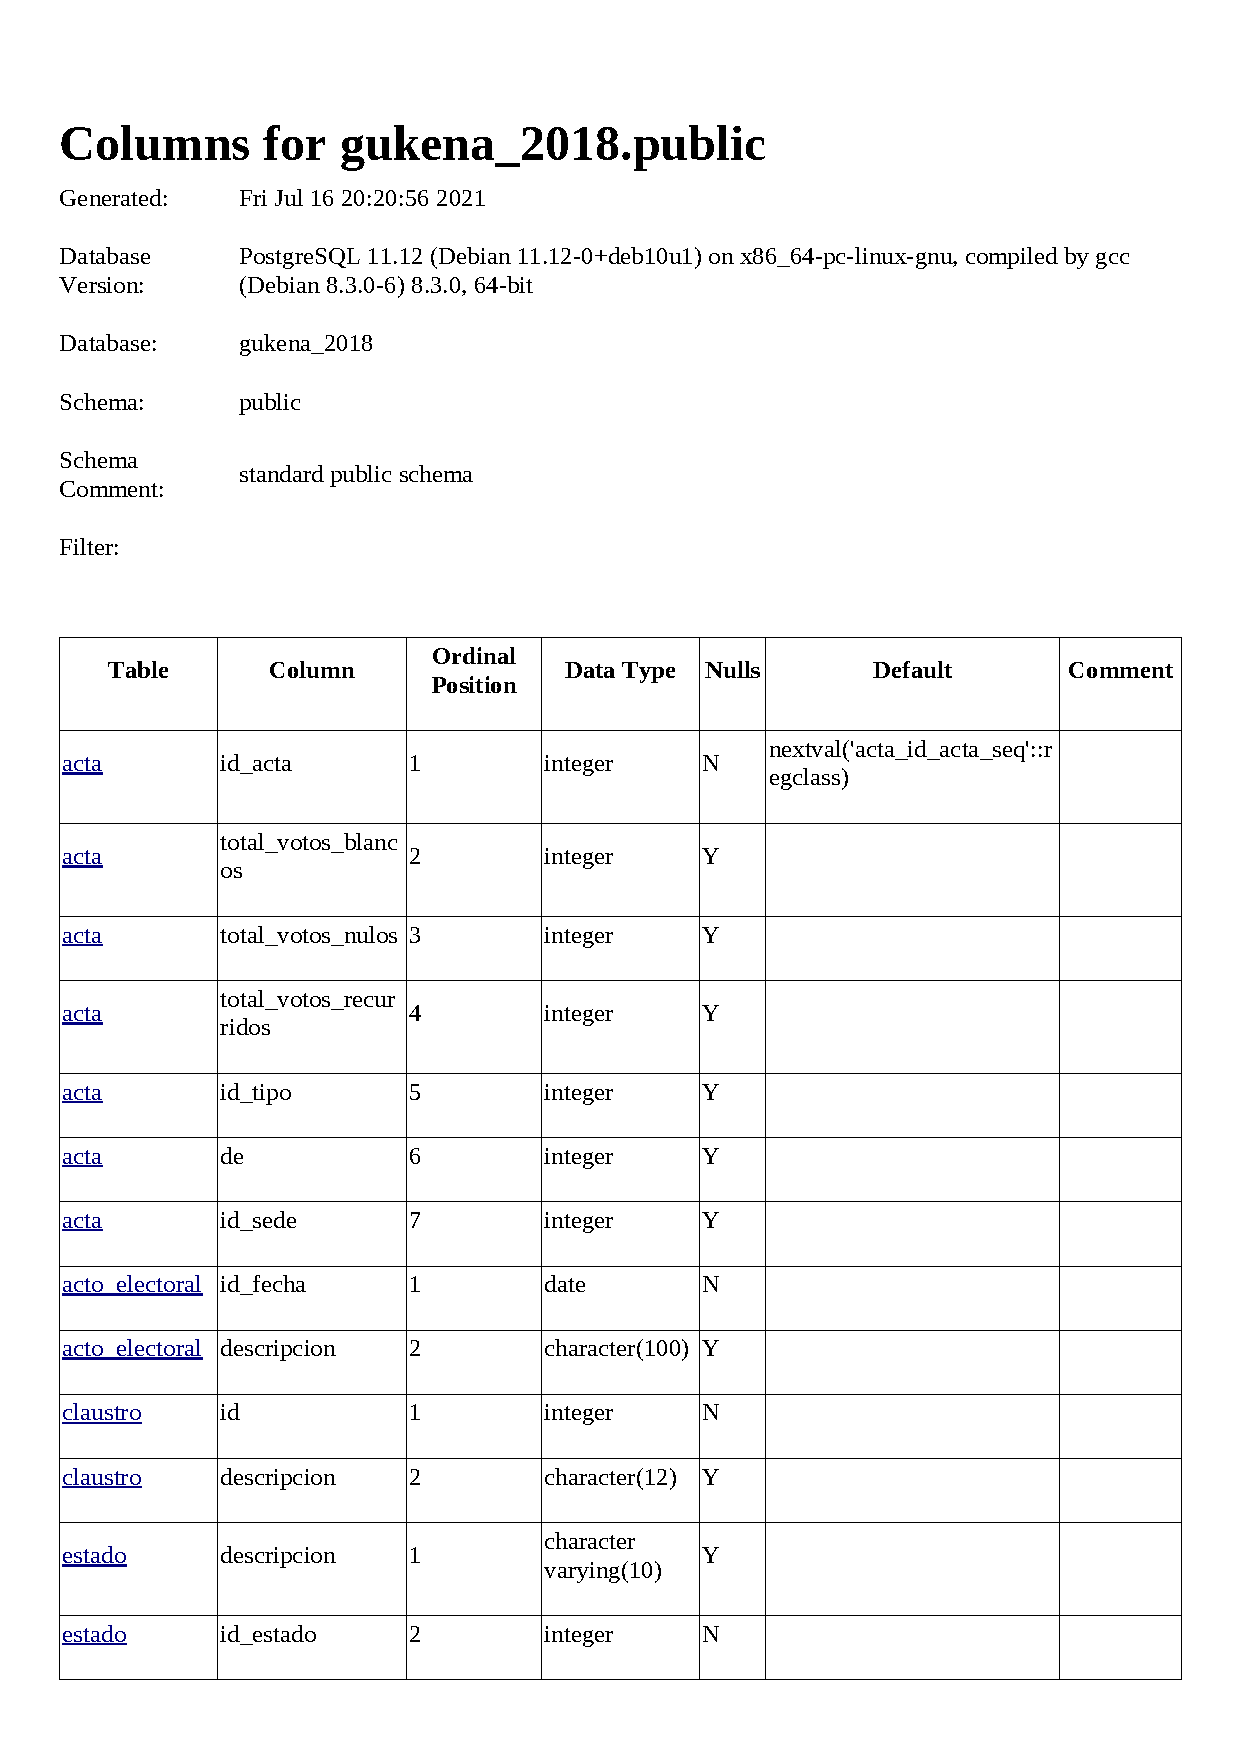
\includepdf[pages=-]{pdf/columns.pdf}

\chapter{Anexo III: Propuesta de la Boleta Única en Papel}
\label{BU}
En esta tesis, se han nombrado experiencias, como es en la provincia de Córdoba y en Bariloche, que incluye la boleta única en papel en el proceso electoral \cite{reglamentoBU}. Esta boleta facilita el escrutinio además de otras ventajas listadas a continuación:
\begin{itemize}
    \item Reduce la manipulación de elementos durante el acto electoral, cumpliendo los requisitos sanitarios. La gran cantidad de papeles y sobres utilizados por cada votante se reducen notablemente. 
    \item En esta boleta se visualizan todos los candidatos de un mismo claustro, siendo equitativo para todos los partidos presentados.
    \item Al reducir la cantidad de papeles por votante, se simplifica el voto y su recuento.
    \item Reduce la posibilidad de fraudes electorales al no dar lugar a boletas falsas, se evita el robo u ocultar boletas, solo la Autoridad de Mesa entrega la boleta habilitada a cada votante durante la votación.
    \item Reduce notablemente la cantidad de elementos utilizados como papeles, sobres y espacio físico. Se podría utilizar el mismo aula tanto para las autoridades de la mesa con un biombo que dé privacidad al votante.
\end{itemize}

A continuación se muestra un ejemplo de una boleta única que podría utilizarse en las elecciones de UNComa.
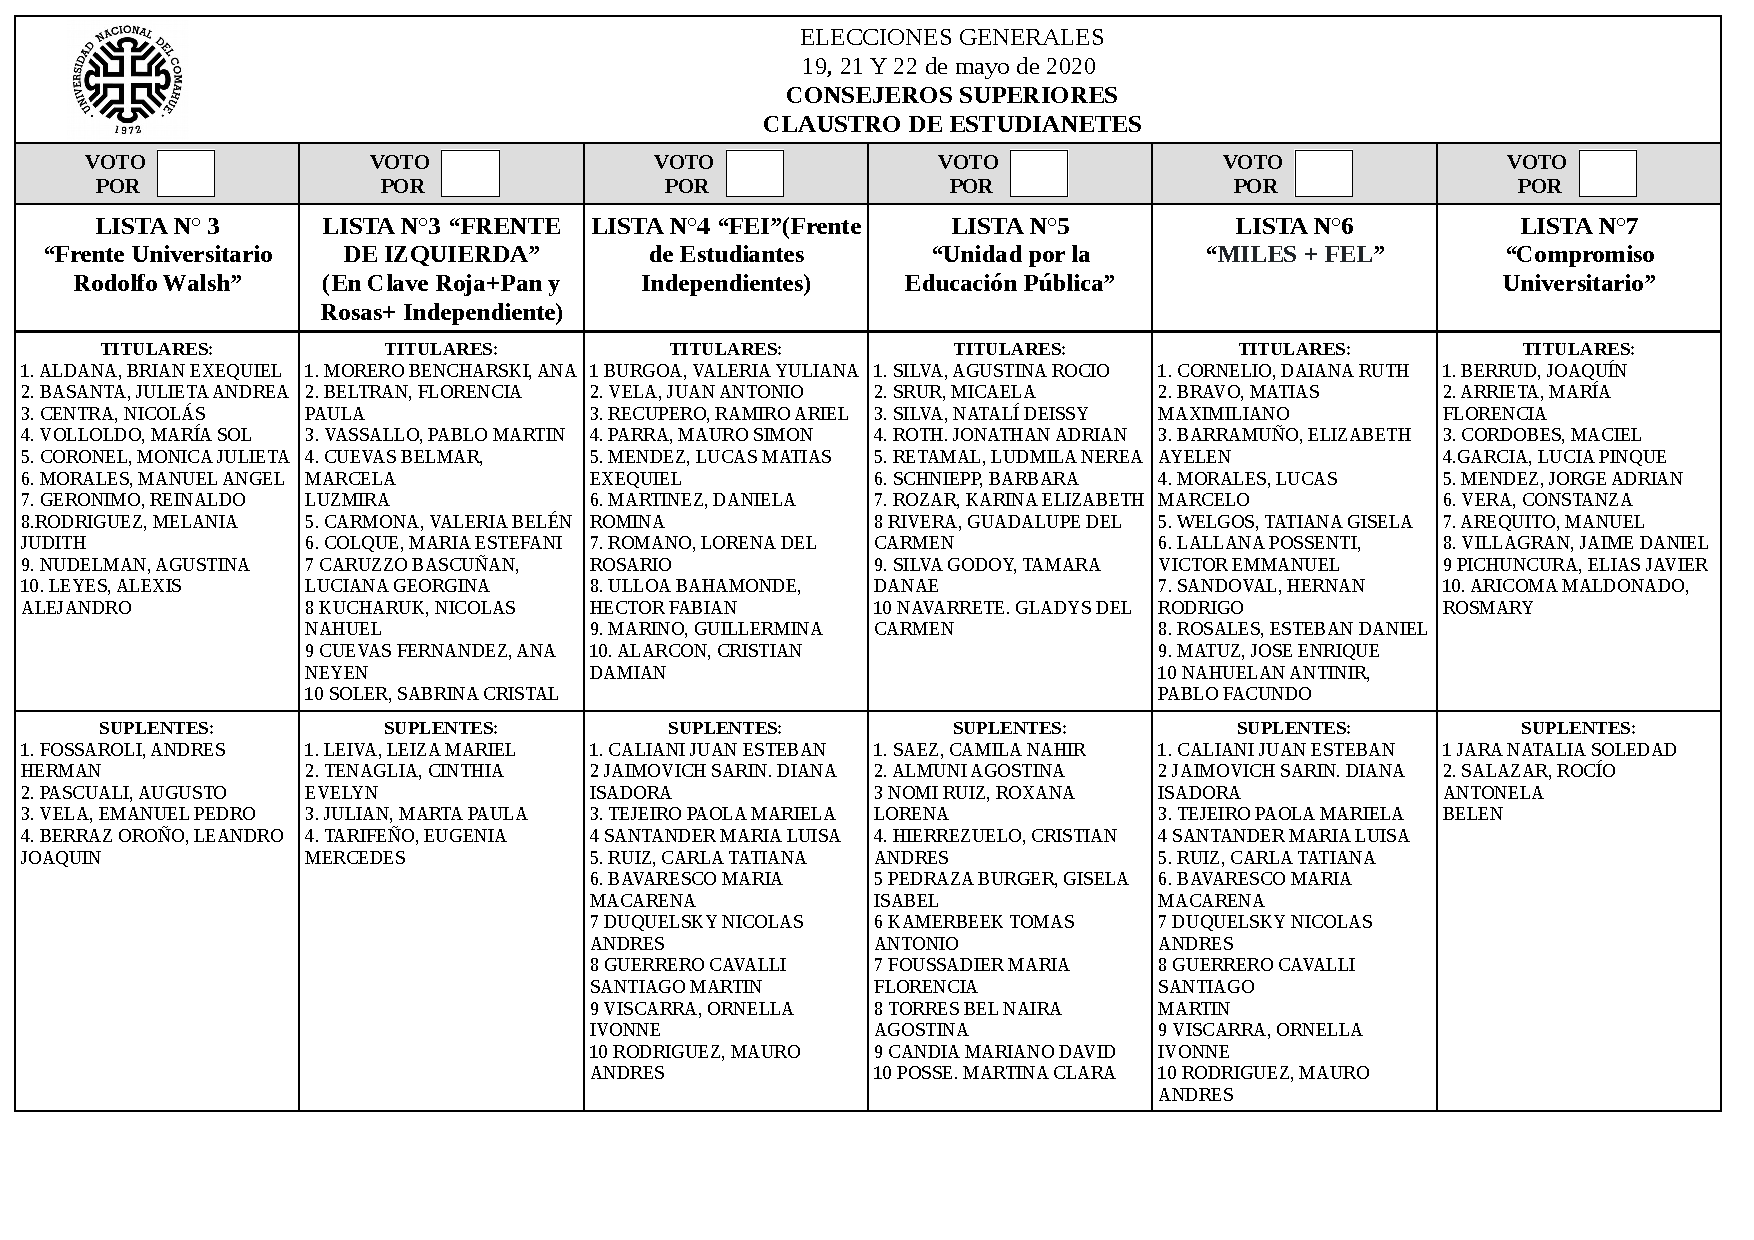
\includepdf[pages=-]{pdf/bue_uncoma.pdf}
%...
\vfill
\newpage

\bibliographystyle{plain}
\bibliography{references}

\end{document}
